\begin{savequote}[75mm]
God does not care about our mathematical difficulties. He integrates empirically.
\qauthor{--- Albert Einstein ---}
\end{savequote}

\chapter{Multiple integrals}
\label{chap_double}
\graphicspath{{figures/Multiple/}}

The previous chapter introduced multivariable functions and we applied concepts of differential calculus to these functions. We learned how we can view a function of two variables as a surface in space, and learned how partial derivatives convey  information about how the surface is changing in any direction.

In this chapter we apply techniques of integral calculus to multivariable functions. In Chapter \ref{chap_int} we learned how the definite integral of a single variable function gave us area under the curve. In this chapter we will see that integration applied to a multivariable function gives us volume under a surface. And just as we learned applications of integration beyond finding areas, we will find applications of integration in this chapter beyond finding volume.

\section{Iterated integrals and area}\label{sec:iterated_integrals}
\subsection{Iterated integrals}
In Chapter \ref{chap_multi_var} we found that it was useful to differentiate functions of several variables with respect to one variable, while treating all the other variables as constants or coefficients. We can integrate functions of several variables in a similar way. For instance, if we are told that $f_x(x,y) = 2xy$, we can treat $y$ as staying constant and integrate to obtain $f(x,y)$:
\begin{align*}
f(x,y) &= \int\limits f_x(x,y)\ dx\\[0.2cm]
				&= \int\limits 2xy\ dx \\[0.2cm]
				&= x^2y + C.
\end{align*}
Make a careful note about the constant of integration, $C$. This ``constant'' is something with a derivative of $0$ with respect to $x$, so it could be any expression that contains only constants and functions of $y$. For instance, if $f(x,y) = x^2y+ \sin (y) + y^3 + 17$, then $f_x(x,y) = 2xy$. To signify that $C$ is actually a function of $y$, we write:

$$f(x,y) = \int\limits f_x(x,y)\ dx  = x^2y+C(y).$$

Using this process we can even evaluate definite integrals. For instance, to evaluate the integral 
$$\ds \int\limits_1^{2y} 2xy\ dx.$$
We find the indefinite integral as before, then apply the fundamental theorem of calculus to evaluate the definite integral:
\begin{align*}
\int\limits_1^{2y} 2xy\ dx &= x^2y\Big|_1^{2y}\\
			&= (2y)^2y - (1)^2y \\
			&= 4y^3-y.
\end{align*}

We can also integrate with respect to $y$. In general,
$$\int\limits_{h_1(y)}^{h_2(y)} f_x(x,y)\ dx = f(x,y)\Big|_{h_1(y)}^{h_2(y)} = f\big(h_2(y),y\big)-f\big(h_1(y),y\big),$$
and
$$\int\limits_{g_1(x)}^{g_2(x)} f_y(x,y)\ dy = f(x,y)\Big|_{g_1(x)}^{g_2(x)} = f\big(x,g_2(x)\big)-f\big(x,g_1(x)\big).$$

Note that when integrating with respect to $x$, the bounds are functions of $y$ (of the form $x=h_1(y)$ and $x=h_2(y)$) and the final result is also a function of $y$. When integrating with respect to $y$, the bounds are functions of $x$ (of the form $y=g_1(x)$ and $y=g_2(x)$) and the final result is a function of $x$. 

When evaluating $\int\limits_1^{2y} 2xy\ dx$,  we integrated a function with respect to $x$ and ended up with a function of $y$. We can integrate this as well. This process is known as iterated integration, or \textbf{multiple integration} (\textit{meervoudige integratie}). Of course,  when considering 
 $$\int\limits_{x_1}^{x_2}\int\limits_{g_1(x)}^{g_2(x)} \ f(x,y) dy\ dx$$
 $x$ should have constant bounds, whereas $y$ may have variable ones, and vice versa when considering
 $$\int\limits_{y_1}^{y_2}\int\limits_{h_1(y)}^{h_2(y)} \ f(x,y) dx\ dy$$

\begin{example}\label{ex_iterated3}
Evaluate 
$$\ds \int\limits_1^2\left(\int\limits_1^x\big(5x^3y^{-3}+6y^2\big)\ dy\right)\ dx.$$

\xhrulefill{gray}{2.5pt}Solution \xhrulefill{gray}{2.5pt}

We follow a standard order of operations and perform the operations inside parentheses first.
\begin{align*}
\int\limits_1^2\left(\int\limits_1^x\big(5x^3y^{-3}+6y^2\big)\ dy\right)\ dx &= \int\limits_1^2 \left(\frac{5x^3y^{-2}}{-2}+\frac{6y^3}{3}\right)\Bigg|_1^x\ dx \\
            & = \int\limits_1^2 \left(\frac{5x^3}{-2x^2}+\frac{6x^3}{3}-\dfrac{5x^3}{-2}-\dfrac{6}{3}\right)\ dx\\
            & = \int\limits_1^2 \left(-\frac{5x}{2}+2x^3+\dfrac{5x^3}{2}-2\right)\ dx\\
            & = \int\limits_1^2 \left(\frac{9x^3}{2}-\dfrac{5x}{2}-2\right)\ dx\\
			&= \left(\frac98x^4-\frac54x^2-2x\right)\Bigg|_1^2\\
			&= \frac{89}8
\end{align*}
Note how the bounds of $x$ were $x=1$ to $x=2$ and the final result was a number.
\end{example}


 

The previous example showed how we could perform something called an iterated integral; we do not yet know why we would be interested in doing so nor what the result, such as the number $89/8$, means. We will now investigate that. 

\subsection{Area of a plane region}

Consider the plane region $R$ bounded by $a\leq x\leq b$ and $g_1(x)\leq y\leq g_2(x)$, shown in Figure \ref{fig_multiple_1a}. We learned in Section \ref{sec:ABC} that the area of $R$ is given by 
\index{integration!area}
$$\int\limits_a^b \big(g_2(x)-g_1(x)\big)\ dx.$$


We can  view the expression $\big(g_2(x)-g_1(x)\big)$ as 
$$\big(g_2(x)-g_1(x)\big) = \int\limits_{g_1(x)}^{g_2(x)} 1\ dy =\int\limits_{g_1(x)}^{g_2(x)} \ dy,$$
meaning we can express the area of $R$ as an iterated integral:
$$\text{area} = \int\limits_a^b \big(g_2(x)-g_1(x)\big)\ dx = \int\limits_a^b\left(\int\limits_{g_1(x)}^{g_2(x)} \ dy\right) dx =\int\limits_a^b\int\limits_{g_1(x)}^{g_2(x)} \ dy\ dx.$$

In short: a certain iterated integral can be viewed as giving the area of a plane region.

A region $R$ could also be defined by $c\leq y\leq d$ and $h_1(y)\leq x\leq h_2(y)$, as shown in Figure \ref{fig_multiple_1b}. Using a process similar to that above, we have 
$$\int\limits_c^d\int\limits_{h_1(y)}^{h_2(y)} \ dx\ dy.$$


\begin{figure}[H]
\centering
%\raisebox{0.5cm}{
\subfigure[\label{fig_multiple_1a}]{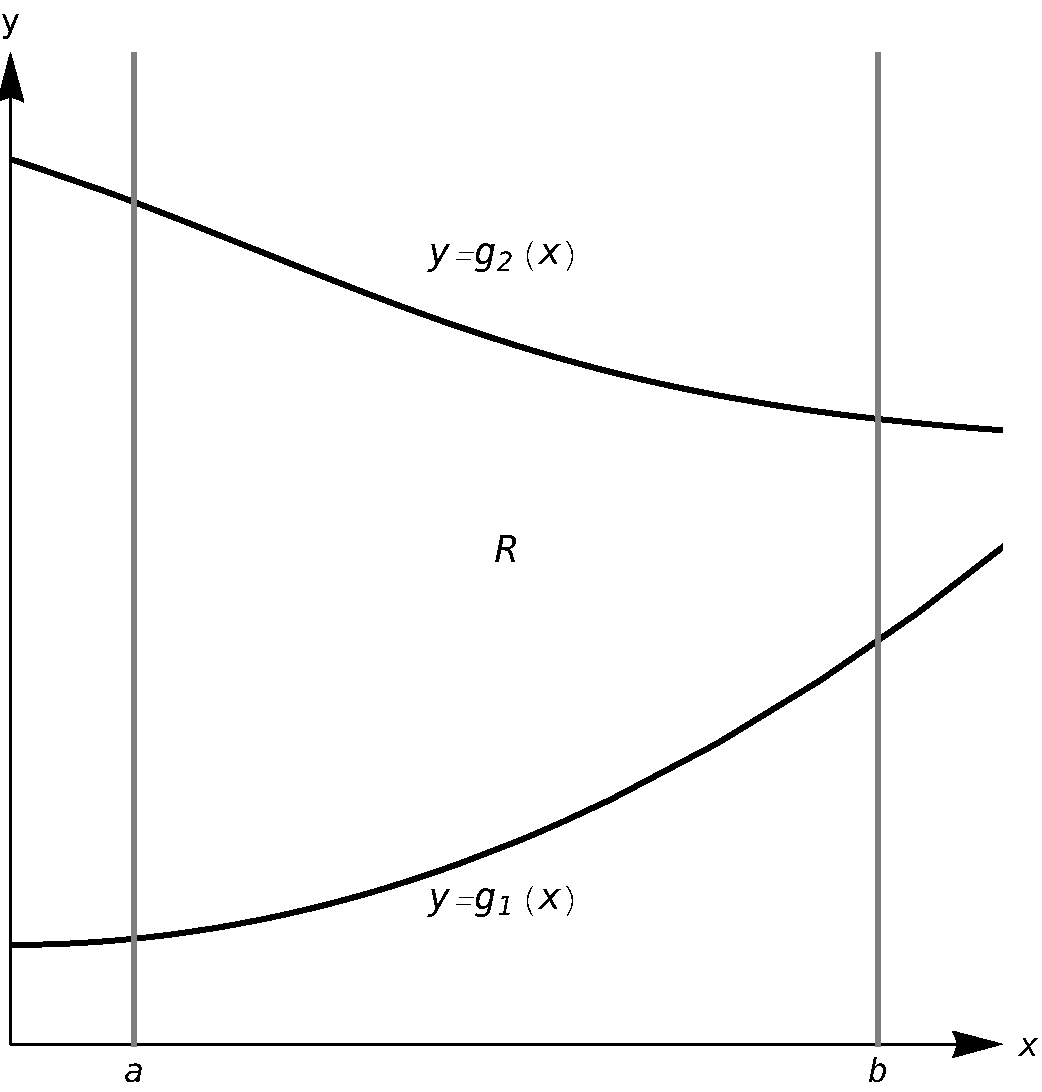
\includegraphics[width=0.43\textwidth]{fig_multiple_1a}}
\qquad
\subfigure[\label{fig_multiple_1b}]{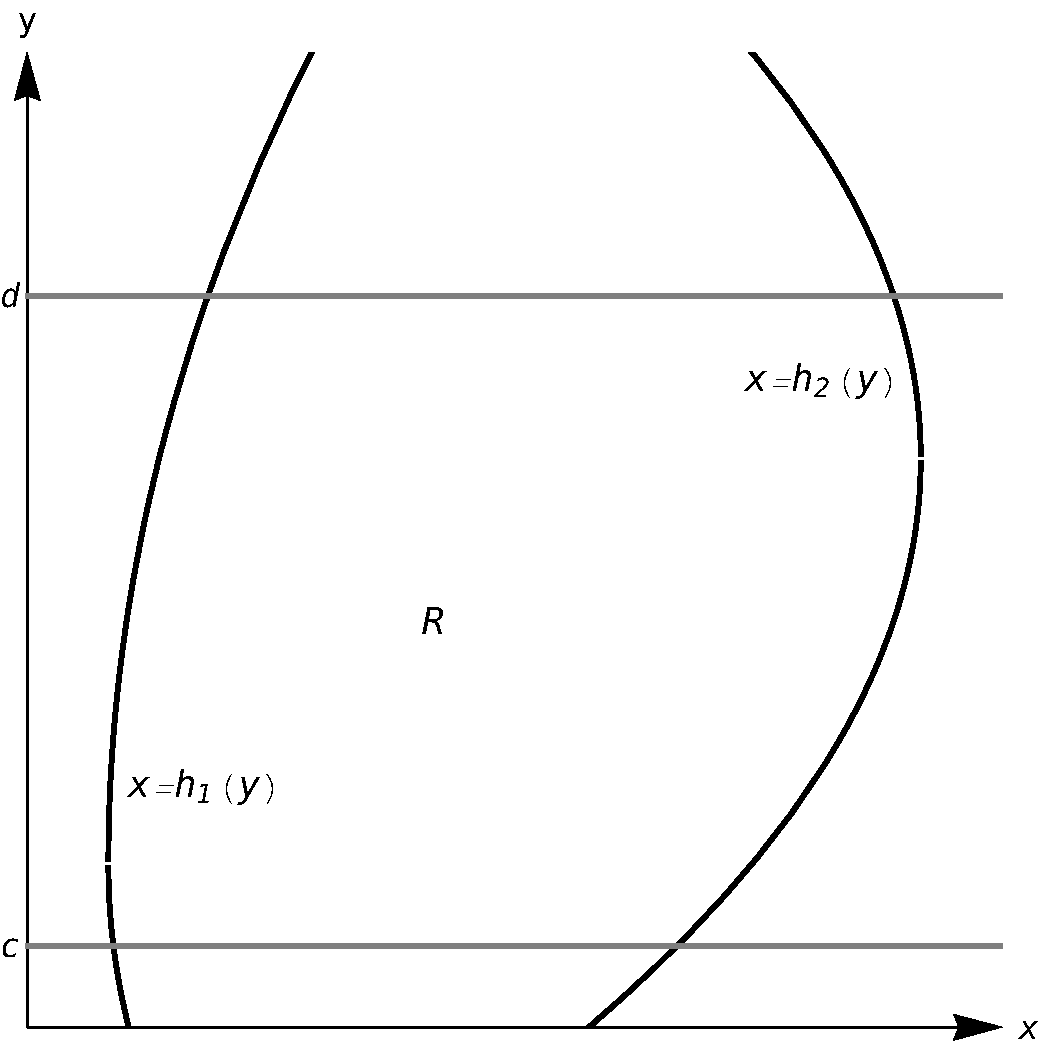
\includegraphics[width=0.43\textwidth]{fig_multiple_1b} }
\caption{Calculating the area of a plane region $R$ with iterated integrals. }
\end{figure}

We state this formally in a theorem.

\begin{theorem}[Area of a plane region]\label{thm:area_plane_region}
\begin{enumerate}[align=left]
	\item Let $R$ be a plane region bounded by $a\leq x\leq b$ and $g_1(x)\leq y\leq g_2(x)$, where $g_1$ and $g_2$ are continuous functions on $[a,b]$. The \textbf{area $A$ of $R$} is
	$$A = \int\limits_a^b\int\limits_{g_1(x)}^{g_2(x)} \ dy\ dx.$$
	\item Let $R$ be a plane region bounded by $c\leq y\leq d$ and $h_1(y)\leq x\leq h_2(y)$, where $h_1$ and $h_2$ are continuous functions on $[c,d]$. The \textbf{area $A$ of $R$} is
	\index{integration!area}
	$$A = \int\limits_c^d\int\limits_{h_1(y)}^{h_2(y)} \ dx\ dy.$$
\end{enumerate}
\end{theorem}

The following examples should help us understand this theorem.


\begin{example}\label{ex_iterated5}
Find the area $A$ of the triangle with vertices at $(1,1)$, $(3,1)$ and $(5,5)$, as shown in Figure \ref{fig_multiple_2a}.



\begin{figure}[H]
\centering
%\raisebox{0.5cm}{
\subfigure[\label{fig_multiple_2a}]{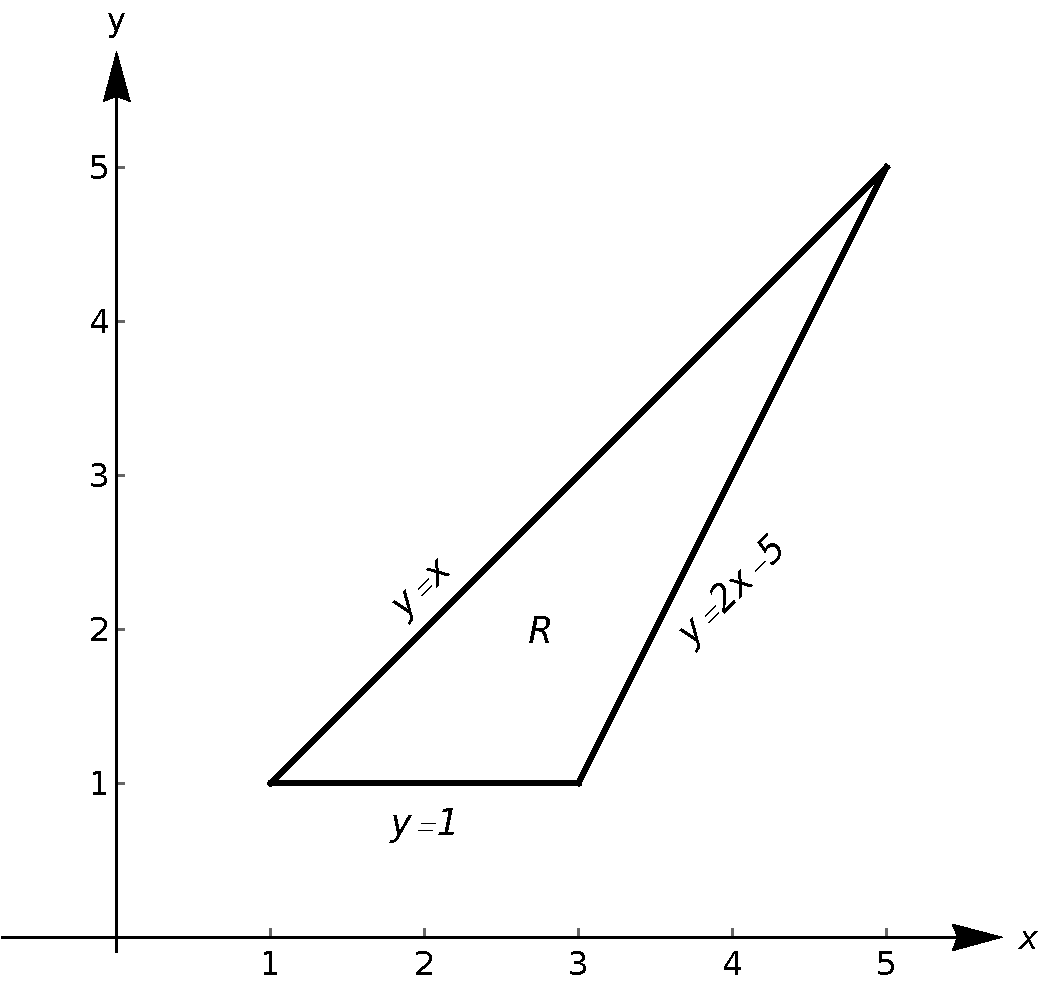
\includegraphics[width=0.4\textwidth]{fig_multiple_2a}}
\qquad
\subfigure[\label{fig_multiple_2b}]{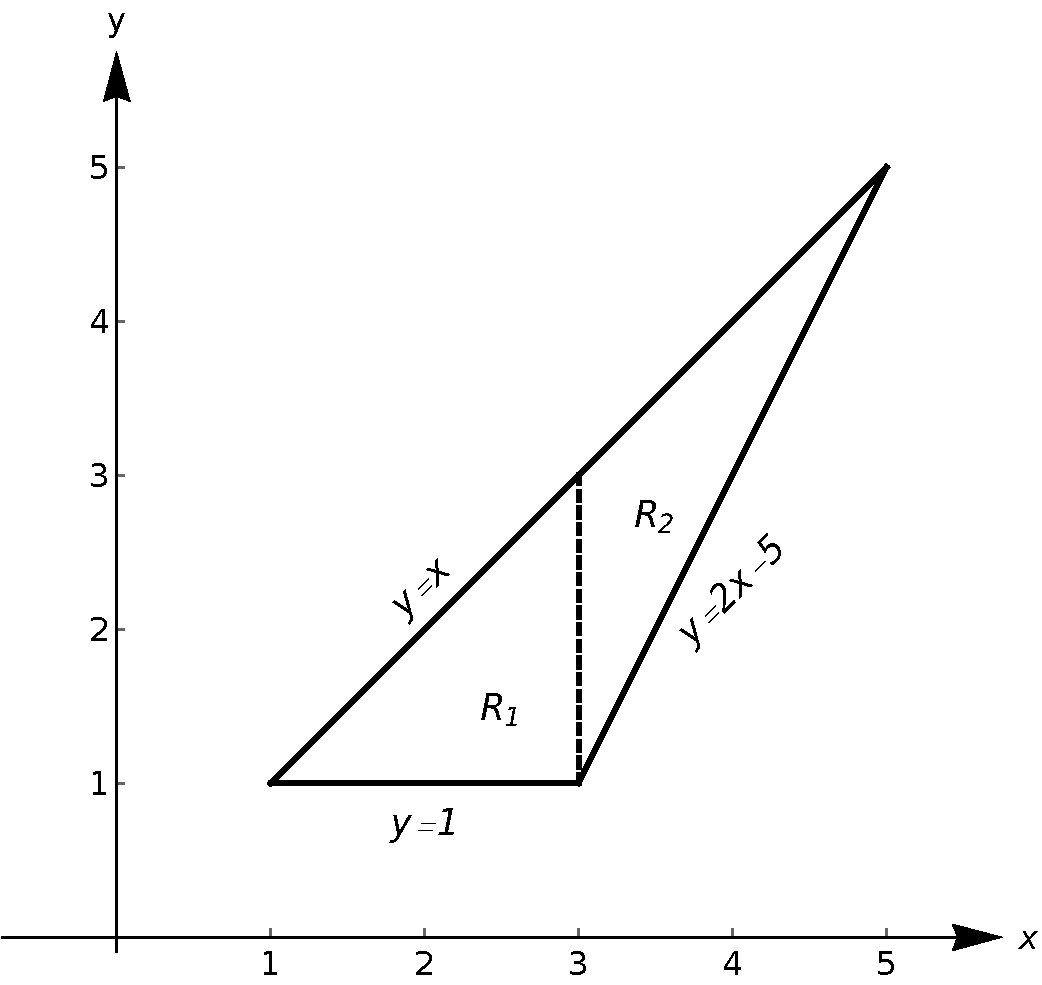
\includegraphics[width=0.4\textwidth]{fig_multiple_2b} }
\caption{Calculating the area of a triangle with iterated integrals in Example \ref{ex_iterated5} by using constant bounds on $y$ (a) and $x$ (b) }
\end{figure}




\xhrulefill{gray}{2.5pt}Solution \xhrulefill{gray}{2.5pt}

The triangle is bounded by the lines as shown in  Figure~\ref{fig_multiple_2a}. Choosing to integrate with respect to $x$ first gives that $x$ is bounded by $x=y$ to $x = \frac{y+5}2$, while $y$ is bounded by $y=1$ to $y=5$, i.e.\ the bounds with respect to $y$ are fixed. Recall that since $x$-values increase from left to right, the leftmost curve, $x=y$, is the lower bound and the rightmost curve, $x=(y+5)/2$, is the upper bound. The area is
\allowdisplaybreaks
\begin{align*}
A &= \int\limits_1^5\int\limits_{y}^{\frac{y+5}2}\ dx\ dy \\
 &= \int\limits_1^5\left(x\right)\ \Big|_y^{\frac{y+5}2}\ dy \\
&= \int\limits_1^5 \left(-\frac12y+\frac52\right)\ dy \\
&= \left(-\frac14y^2+\frac52y\right)\Bigg|_1^5\\
&=4.
\end{align*}

We can also find the area by integrating with respect to $y$ first, which implies that the bounds on $y$ are variable and dependent on $x$, whereas the one on $x$ are fixed. In this situation, though, there is not one function that defines the lower bound on the interval $[1,5]$. Essentially, we have two functions that act as the lower bound for the region $R$, $y=1$ and $y=2x-5$. In this way, the region $R$ is split into two smaller regions, namely $R_1$ and $R_2$ ( Figure~\ref{fig_multiple_2b}). This requires us to use two iterated integrals. Note how the $x$-bounds are different for each integral:
\begin{align*}
A &= \int\limits_1^3\int\limits_1^x 1\ dy \ dx +  \int\limits_3^5\int\limits_{2x-5}^x1\ dy\ dx\\
	&= \int\limits_1^3 y\ \Big|_1^x\ dx  + \int\limits_3^5 y \  \Big|_{2x-5}^x\ dx\\
	&= \int\limits_1^3\big(x-1\big)\ dx  +  \int\limits_3^5\big(-x+5\big)\ dx \\
	&= 2  +  2 \\
	&=4.
\end{align*}
As expected, we get the same answer both ways.
\end{example}

\begin{example}\label{ex_iterated6}
Find the area of the region enclosed by $y=2x$ and $y=x^2$, as shown in Figure \ref{fig_multiple_3}. 



\begin{figure}[H]
	\begin{center}
			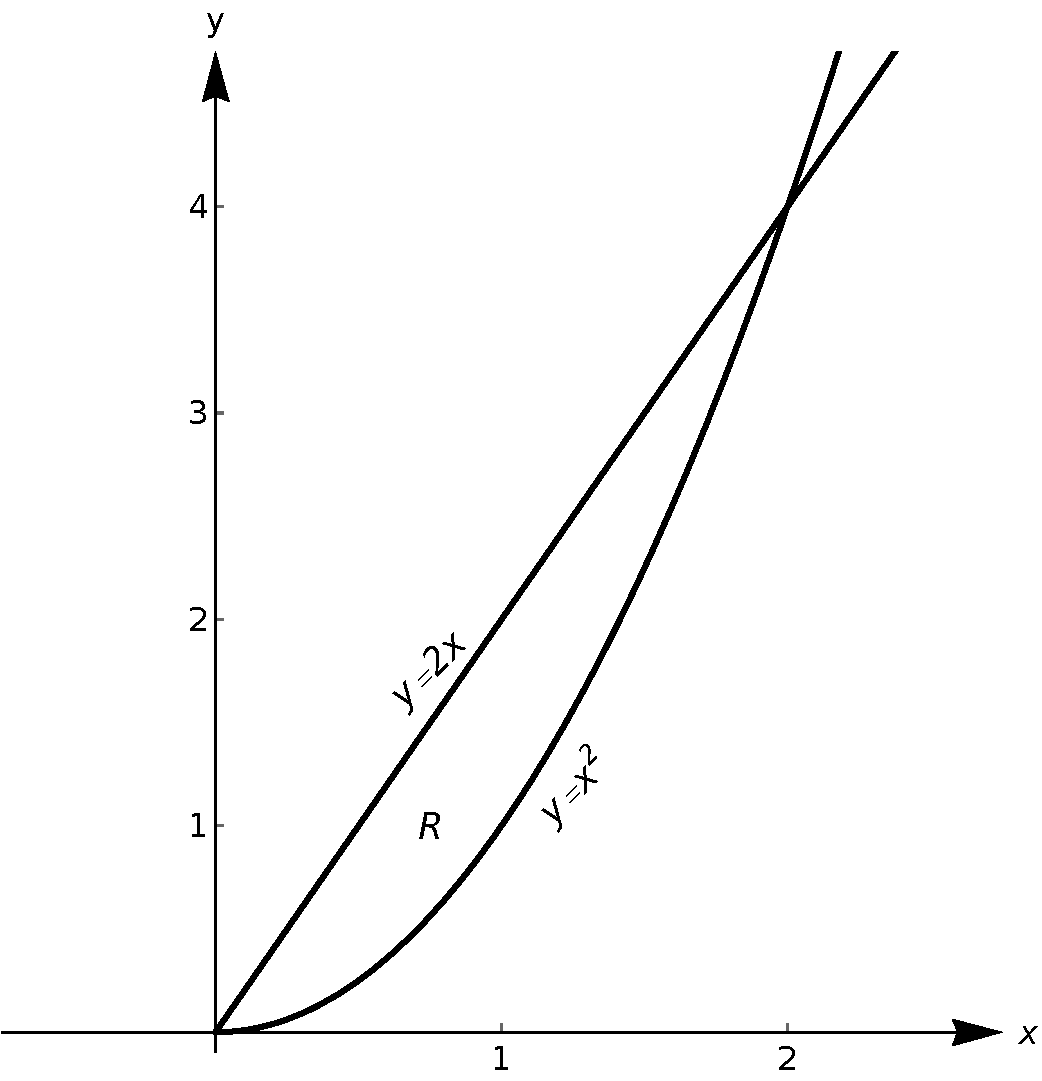
\includegraphics[width=0.4\textwidth]{fig_multiple_3}
	\caption{Calculating the area of a plane region with iterated integrals in Example \ref{ex_iterated6}.}
	\label{fig_multiple_3}
	\end{center}
\end{figure}

\xhrulefill{gray}{2.5pt}Solution \xhrulefill{gray}{2.5pt}

Once again we will find the area of the region using both orders of integration. We can approach this problem in two ways, either by choosing  fixed bounds for $x$ and variable ones - depending on $x$ - for $y$ or by choosing fixed bounds for $y$ and variable ones for $x$, which then depend on $y$. So, in the former case, we first integrate with respect to $y$ and then with respect to $x$:
$$\int\limits_0^2\int\limits_{x^2}^{2x}1\ dy \ dx = \int\limits_0^2(2x-x^2)\ dx = \left(x^2-\frac13x^3\right)\Bigg|_0^2 = \frac43.$$

In the latter case, we, however, do exactly the opposite:
$$\int\limits_0^4\int\limits_{y/2}^{\sqrt{y}} 1\ dx\ dy = \int\limits_0^4 \left(\sqrt{y}-\dfrac{y}{2} \right)\ dy = \left(\frac23y^{3/2} - \frac14y^2\right)\Big|_0^4 = \frac43.$$
\end{example}


In each of the previous examples, we have been given a region $R$ and found the bounds needed to find the area of $R$ using both orders of integration. We integrated using both orders of integration to demonstrate their equality.

We now approach the skill of describing a region using both orders of integration from a different perspective. Instead of starting with a region and creating iterated integrals, we will start with an iterated integral and rewrite it in the other integration order. To do so, we will need to understand the region over which we are integrating.

The simplest of all cases is when both integrals are bound by constants. The region described by these bounds is a rectangle, and so:
$$\int\limits_a^b\int\limits_c^d 1\ dy\ dx = \int\limits_c^d\int\limits_a^b1\ dx\ dy.$$

	\checkoddpage
\marginpar{\ifoddpage\hspace*{-1.5cm}\else\hspace*{0.25cm}\fi
\includegraphics[width=0.075\textwidth]{youtube}\\
\ifoddpage\hspace*{-1.75cm}\else\hspace*{0.1cm}\fi
\qrcode[height=1.75cm]{https://youtu.be/NETmfwOAKpQ}
%\includegraphics[width=0.1\textwidth]{order_int}
}
When the inner integral's bounds are not constants, it is generally very useful to sketch the bounds to determine what the region we are integrating over looks like. From the sketch we can then rewrite the integral with the other order of integration.

\begin{example}\label{ex_double7}
Change the order of integration of $$\ds\int\limits_0^4\int\limits_{y^2/4}^{(y+4)/2}1\ dx\ dy.$$

\xhrulefill{gray}{2.5pt}Solution \xhrulefill{gray}{2.5pt}

We sketch the region described by the bounds to help us change the integration order. $x$ is bounded below and above (i.e., to the left and right) by $x=y^2/4$ and $x=(y+4)/2$ respectively, and $y$ is bounded between 0 and 4. Graphing the previous curves, we find the region $R$ to be that shown in Figure \ref{fig_multiple_4a}. 


To change the order of integration, we need to give $x$ fixed bounds. The figure makes it clear that there are two lower bounds for $y$: $y=0$ on $0\leq x\leq 2$, and $y=2x-4$ on $2\leq x\leq 4$, thereby splitting $R$ in two smaller regions $R_1$ and $R_2$ (Figure \ref{fig_multiple_4b}). Thus we need two double integrals. The upper bound for each is $y=2\sqrt{x}$. Thus we have
$$\int\limits_0^4\int\limits_{y^2/4}^{(y+4)/2}1\ dx\ dy = \int\limits_0^2\int\limits_0^{2\sqrt{x}} 1\ dy\ dx + \int\limits_2^4\int\limits_{2x-4}^{2\sqrt{x}}1\ dy\ dx.$$



\begin{figure}[H]
\centering
%\raisebox{0.5cm}{
\subfigure[\label{fig_multiple_4a}]{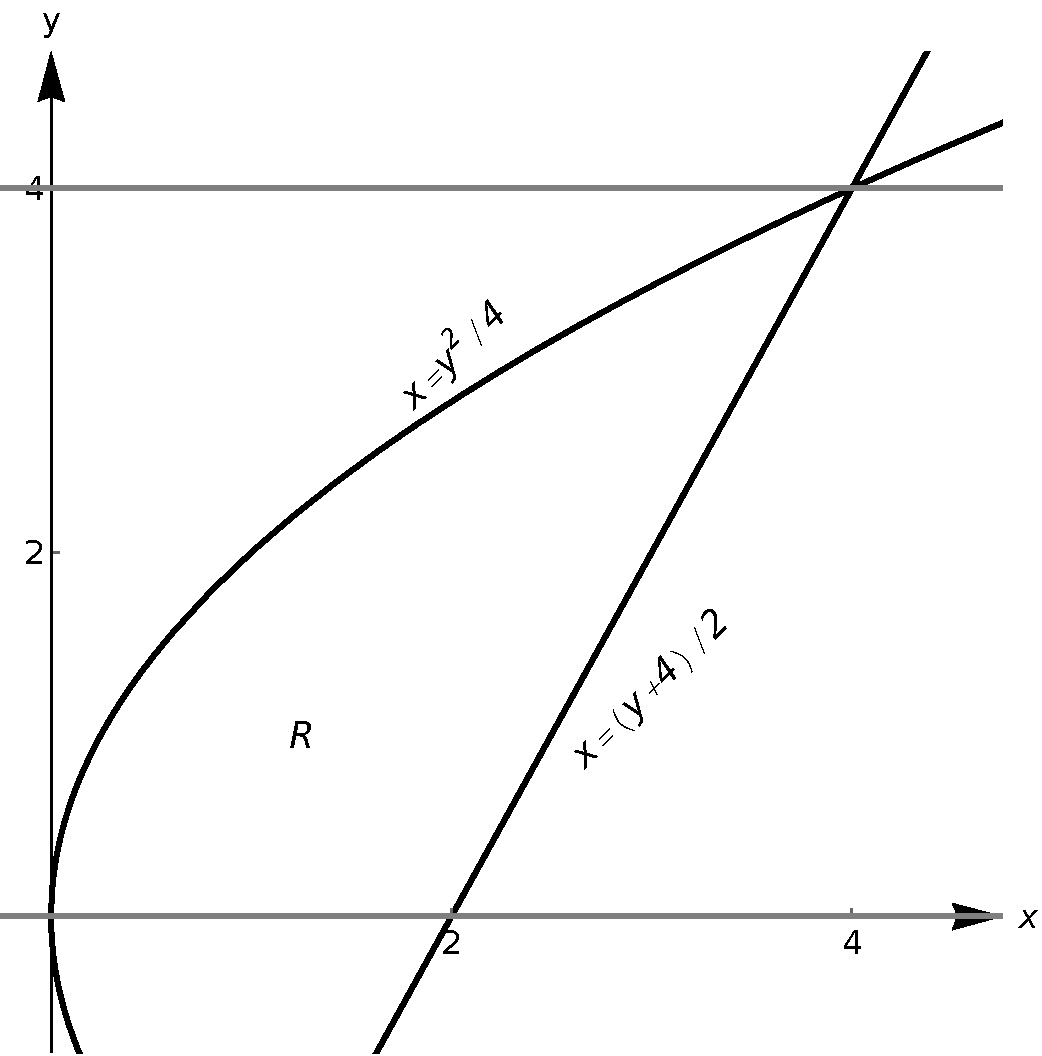
\includegraphics[width=0.4\textwidth]{fig_multiple_4a}}
\qquad
\subfigure[\label{fig_multiple_4b}]{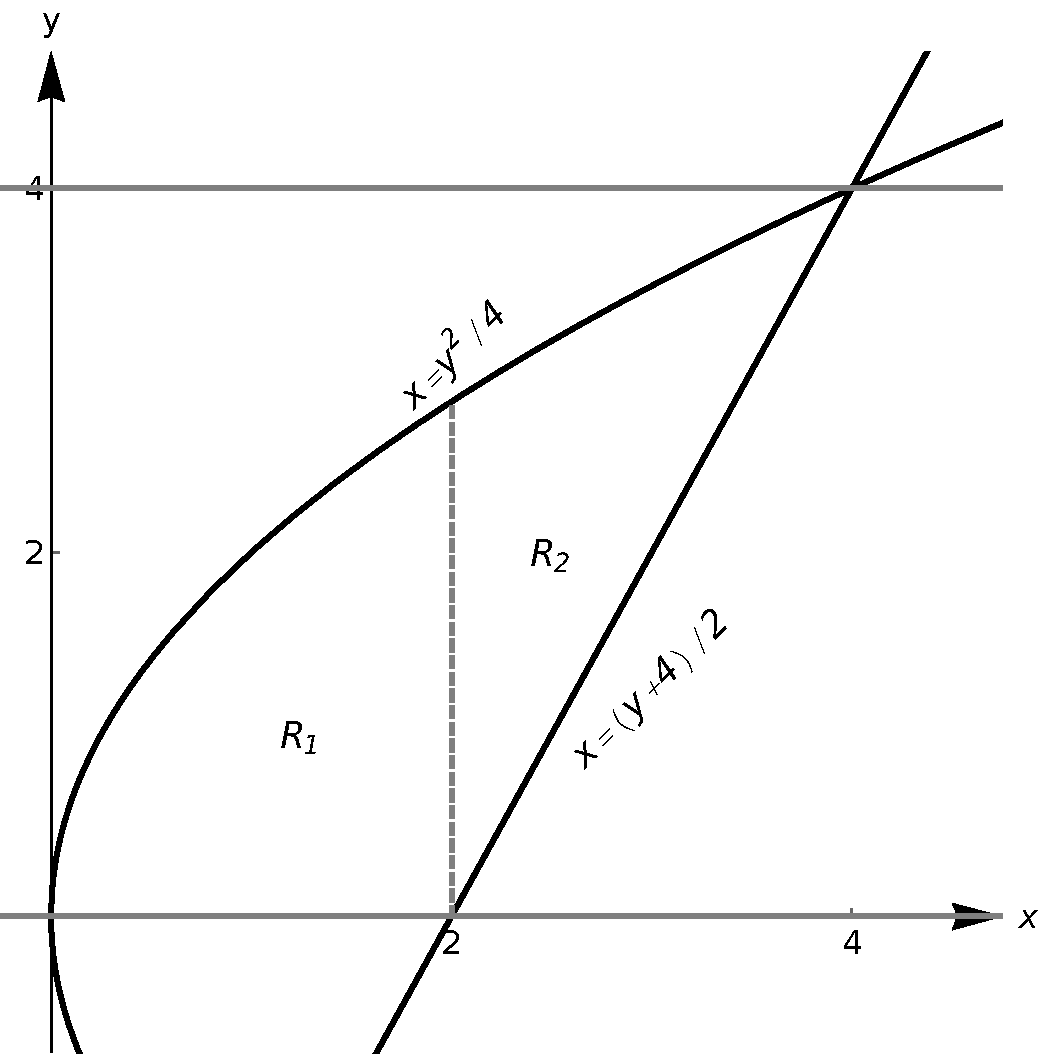
\includegraphics[width=0.4\textwidth]{fig_multiple_4b} }
\caption{Drawing the region determined by the bounds of integration in Example \ref{ex_double7}. }
\end{figure}


\end{example}

This section has introduced a new concept, the iterated integral. We developed one application for iterated integration: area between curves. However, this is not new, for we already know how to find areas bounded by curves. In the next section we apply iterated integration to solve problems we currently do not know how to handle. 


\section{Double integration and volume}\label{sec:double_int_volume}
\subsection{Definition}

The definite integral of $f$ over $[a,b]$, $\int\limits_a^b f(x)\ dx$, was introduced as the signed area under the curve. We approximated the value of this area by first subdividing $[a,b]$ into $n$ subintervals, where the $i^\text{ th}$ subinterval has length $\dx_i$, and letting $c_i$ be any value in the $i^\text{ th}$ subinterval. We formed rectangles that approximated part of the region under the curve with width $\dx_i$, height $f(c_i)$, and hence with area $f(c_i)\dx_i$. Summing all the rectangle's areas gave an approximation of the definite integral, and Theorem \ref{thm:riemann_sum} stated that
$$\int\limits_a^bf(x)\ dx = \lim_{\mathcal{L}\to 0}\sum\limits^{n}_{i=1} f(c_i)\dx_i,$$
connecting the area under the curve with sums of the areas of rectangles. Recall that $\mathcal{L}$ is the  size of the partition, which is the length of the largest subinterval of the partition, i.e. $\mathcal{L}=\max\limits_i\left(\Delta x_i\right)$.

We use a similar approach in this section to find volume under a surface. Let $R$ be a closed, bounded region in the $xy$-plane and let $z=f(x,y)$ be a continuous function defined on $R$. We wish to find the signed volume under the surface of $f$ over $R$. We use the term signed volume to denote that space above the $xy$-plane, under $f$, will have a positive volume; space above $f$ and under the $xy$-plane will have a negative volume, similar to the notion of signed area used before.

We start by partitioning $R$ into $n$ rectangular subregions as shown in Figure \ref{fig_multiple_5a}. For simplicity's sake, we let all widths be $\dx$ and all heights be $\dy$. Note that the sum of the areas of the rectangles is not equal to the area of $R$, but rather is a close approximation. Arbitrarily number the rectangles 1 through $n$, and pick a point $(x_i,y_i)$ in the $i^\text{ th}$ subregion. 


\begin{figure}
\centering
%\raisebox{0.5cm}{
\subfigure[\label{fig_multiple_5a}]{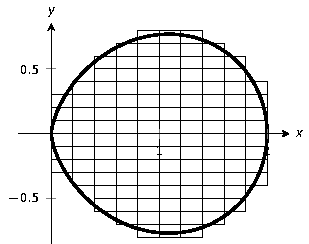
\includegraphics[width=0.43\textwidth]{fig_multiple_5a}}
\qquad
\subfigure[\label{fig_multiple_5b}]{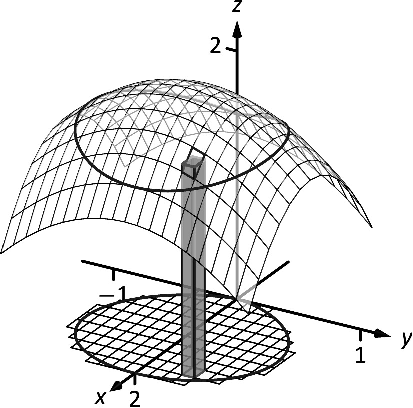
\includegraphics[width=0.43\textwidth]{fig_multiple_5b} }
\caption{Developing a method for finding signed volume under a surface. }
\end{figure}



The volume of the rectangular solid whose base is the $i^\text{ th}$ subregion and whose height is $f(x_i,y_i)$ is $V_i=f(x_i,y_i)\dx\dy$. Such a  solid is shown in Figure \ref{fig_multiple_5b}. Note how this rectangular solid only approximates the true volume under the surface; part of the solid is above the surface and part is below.

For each subregion $R_i$ used to approximate $R$, create the rectangular solid with base area $\dx\dy$ and height $f(x_i,y_i)$. 
The sum of all rectangular solids is $$\ds \sum_{i=1}^n f(x_i,y_i)\dx\dy.$$ This approximates the signed volume under $f$ over $R$. As we have done before, to get a better approximation we can use more rectangles to approximate the region $R$.

In general, each rectangle could have a different width $\dx_j$ and height $\dy_k$, giving the $i^\text{ th}$ rectangle an area $\Delta A_i = \dx_j\dy_k$ and the $i^\text{ th}$ rectangular solid a volume of $f(x_i,y_i)\Delta A_i$. Let now $\mathcal{A}$ denote the length of the longest diagonal of all rectangles in the subdivision of $R$; $\mathcal{A}\to 0$ means each rectangle's width and height are both approaching 0. If $f$ is a continuous function, as $\mathcal{A}$ shrinks (and hence $n\to +\infty$) the summation $\ds \sum_{i=1}^n f(x_i,y_i)\Delta A_i$ approximates the signed volume better and better. 

 When adding up the volumes of rectangular solids over a partition of a region $R$, as done in Figure \ref{fig_multiple_5b}, one could first add up the volumes across each row (one type of sum), then add these totals together (another sum), as in
$$\sum_{j=1}^n\sum_{i=1}^mf(x_i,y_j)\Delta x_i\Delta y_j.$$
One can rewrite this  as
$$\sum_{j=1}^n\left(\sum_{i=1}^mf(x_i,y_j)\Delta x_i\right)\Delta y_j.$$
The summation inside the parenthesis indicates the sum of (heights $\times$ widths), which gives an area; multiplying these areas by the thickness $\Delta y_j$ gives a volume. The illustration in Figure \ref{fig_multiple_5b} relates to this understanding.

This all leads us to a definition.

\begin{definition}[Double integral and signed volume]\label{def:double_int}
Let $z=f(x,y)$ be a continuous function defined over a closed, bounded region $R$ in the $xy$-plane. The \textbf{signed volume $V$ under $f$ over $R$} is denoted by the \textbf{double integral} (\textit{dubbelintegraal})
$$V = \iint_R f(x,y)\ dA.$$
\index{integration!double}\index{double integral}\index{signed volume}\index{volume}
\index[aut]{volume}\index[aut]{dubbelintegraal}
\end{definition}

Alternate notations for the double integral are

$$\iint_R f(x,y)\ dA=\iint_R f(x,y)\ dx\ dy=\iint_R f(x,y)\ dy\ dx.$$

We can find the signed volume by considering increasingly smaller, so more, rectangles; that is by considering the limit
$$\lim_{\mathcal{A}\to 0}\sum_{i=1}^n f(x_i,y_i)\Delta A_i.$$
In this limiting situation, it holds that 
\begin{equation}
V = \iint_R f(x,y)\ dA = \lim_{\mathcal{A}\to 0}\sum_{i=1}^n f(x_i,y_i)\Delta A_i.
\label{thm:double_int}
\end{equation}

Note that this equation does not specify the partition of the region $R$, so any partitioning where the diagonal of each rectangle shrinks to 0 results in the same answer. This does not offer a very satisfying way of computing volume, though. Our experience has shown that evaluating the limits of sums can be tedious. We seek a more direct method.

Recall Theorem \ref{thm:volume_by_cross_section}. This stated that if $A(x)$ gives the cross-sectional area of a solid at $x$, then $\int\limits_a^b A(x)\ dx$ gave the volume of that solid over $[a,b]$. Consider Figure \ref{fig_multiple_6}, where a surface $z=f(x,y)$ is drawn over a region $R$. Fixing a particular $x$-value, we can consider the area under $f$ over $R$ where $x$ has that fixed value. That area can be found with a definite integral, namely 
$$ 
A(x)=\int\limits_{g_1(x)}^{g_2(x)} f(x,y)\ dy.
$$


\begin{figure}
	\begin{center}
			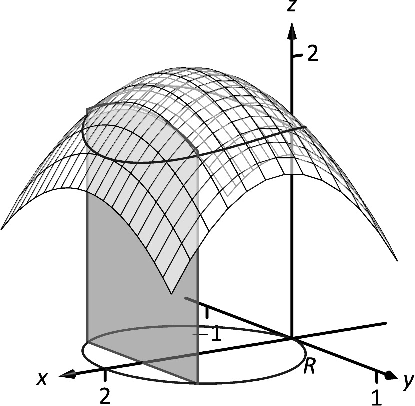
\includegraphics[width=0.5\textwidth]{fig_multiple_6}
	\caption{Finding volume under a surface by sweeping out a cross--sectional area.}
	\label{fig_multiple_6}
	\end{center}
\end{figure}

Remember that though the integrand contains $x$, we are viewing $x$ as fixed. Also note that the bounds of integration are functions of $x$: the bounds depend on the value of $x$. As $A(x)$ is a cross-sectional area function, we can find the signed volume $V$ under $f$ by integrating it:
$$V = \int\limits_a^b A(x)\ dx = \int\limits_a^b\left(\int\limits_{g_1(x)}^{g_2(x)} f(x,y)\ dy\right)dx = \int\limits_a^b\int\limits_{g_1(x)}^{g_2(x)} f(x,y)\ dy\ dx.$$

This gives a concrete method for finding signed volume under a surface. We could do a similar procedure where we started with $y$ fixed, resulting in an iterated integral with the order of integration $dx\ dy$. The following theorem states that both methods give the same result, which is the value of the double integral. It is such an important theorem it has a name associated with it.

\begin{theorem}[Fubini's theorem]\label{thm:fubini}
Let $R$ be a closed, bounded region in the $xy$-plane and let $z=f(x,y)$ be a continuous function on $R$.%
\index{double integral}\index{iterated integration}\index{signed volume}\index{volume}\index{Fubini's Theorem}\index[aut]{stelling van Fubini}
\begin{enumerate}[align=left]
	\item If $R$ is bounded by $a\leq x\leq b$ and $g_1(x)\leq y\leq g_2(x)$, where $g_1$ and $g_2$ are continuous functions on $[a,b]$, then
	$$\iint_R f(x,y)\ dA = \int\limits_a^b\int\limits_{g_1(x)}^{g_2(x)} f(x,y)\ dy\ dx.$$
	
	\item If $R$ is bounded by $c\leq y\leq d$ and $h_1(y)\leq x\leq h_2(y)$, where $h_1$ and $h_2$ are continuous functions on $[c,d]$, then
	$$\iint_R f(x,y)\ dA = \int\limits_c^d\int\limits_{h_1(y)}^{h_2(y)} f(x,y)\ dx\ dy.$$
\end{enumerate}
\end{theorem}

\ifanalysis
\begin{proof}
We state this theorem without proof because it is rather technical, but it is important to realize that it is valid only if 
$$\iint_R \left|f(x,y)\right|\ dA<+\infty\,,$$
which is fulfilled if $R$ is a closed, bounded region on which $z=f(x,y)$ is a continuous function. 
\end{proof}
\fi

\begin{example}\label{ex_double1}
Let $f(x,y) = xy+e^y$. Find the signed volume under $f$ on the region $R$, which is the rectangle with corners $(3,1)$ and $(4,2)$ pictured in Figure \ref{fig_multiple_7}, using both orders of integration.

\pagebreak
\xhrulefill{gray}{2.5pt}Solution \xhrulefill{gray}{2.5pt}


\begin{figure}[H]
	\begin{center}
			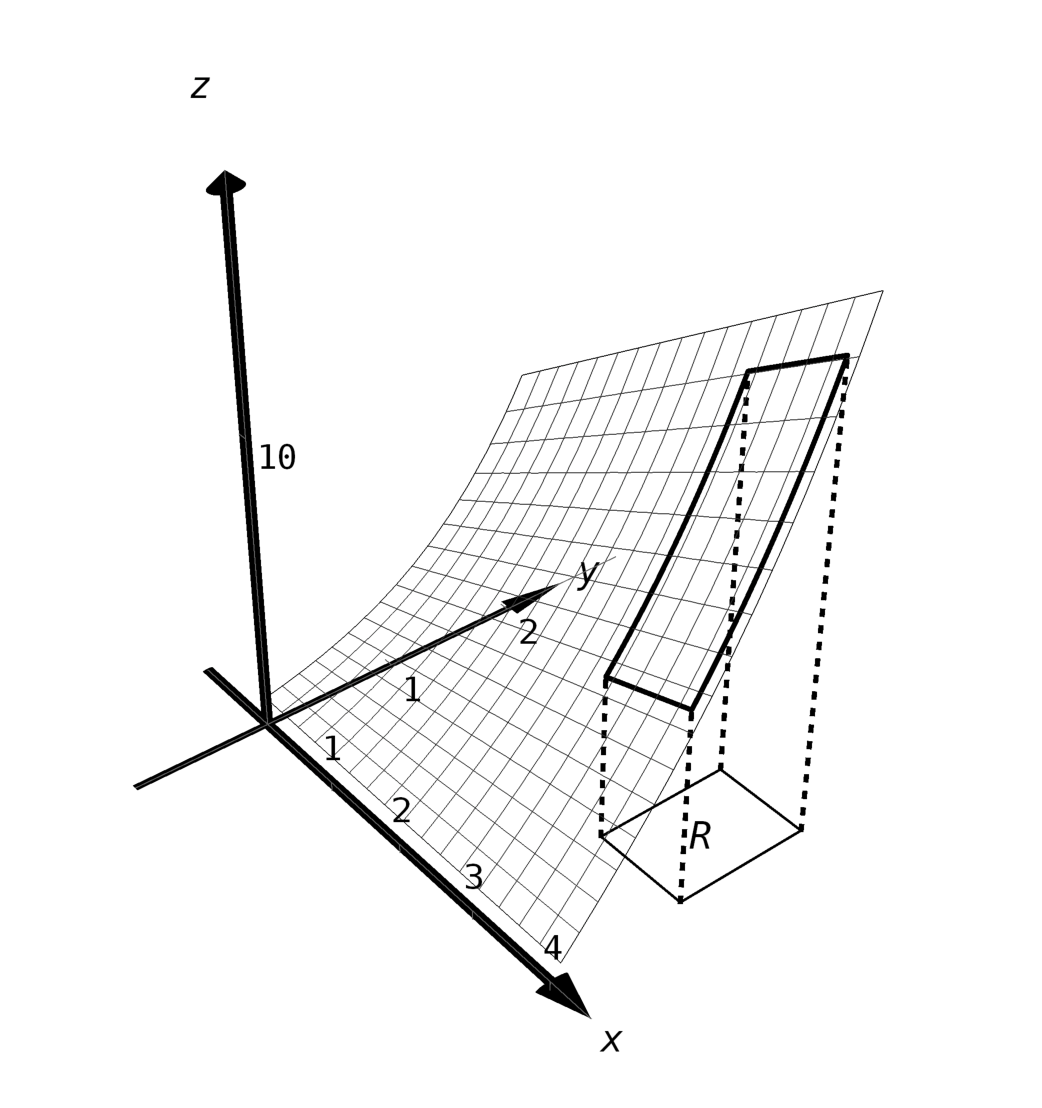
\includegraphics[width=0.55\textwidth]{fig_multiple_7}
	\caption{Finding the signed volume under a surface in Example \ref{ex_double1}.}
	\label{fig_multiple_7}
	\end{center}
\end{figure}


We wish to evaluate $\iint_R \big(xy+e^y\big)\ dA$. As $R$ is a rectangle, the bounds are easily described as $3\leq x\leq 4$ and $1\leq y\leq 2$.\\

Using the order $dy\ dx$:
\begin{align*}
\iint_R\big(xy+e^y\big) \ dA &= \int\limits_3^4\int\limits_1^2\big(xy+e^y\big)\ dy \ dx \\
			&= \int\limits_3^4 \left.\left(\frac12xy^2+e^y\right)\right|_1^2\  dx \\
			&= \int\limits_3^4\left(\frac 32x + e^2-e\right)\ dx \\
			&= \left.\left(\frac 34x^2 + \big(e^2-e\big)x\right)\right|_3^4 \\
			&= \frac {21}4+ e^2-e\approx 9.92.
\end{align*}


Now we check the validity of Fubini's theorem by using the order $dx\ dy$:
\allowdisplaybreaks
\begin{align*}
\iint_R\big(xy+e^y\big) \ dA &= \int\limits_1^2\int\limits_3^4\big(xy+e^y\big)\ dx \ dy \\
		&= \int\limits_1^2\left.\left(\frac12x^2y+xe^y\right)\right|_3^4\ dy\\
		&= \int\limits_1^2\left(\frac72y+e^y\right)\ dy\\
		&= \left.\left(\frac74y^2+e^y\right)\right|_1^2\\
		&=\frac{21}4+e^2-e\approx 9.92.
\end{align*}
Both orders of integration return the same result, as expected.
\end{example}


\begin{example}\label{ex_double2}
Evaluate $$\iint_R \big(3xy-x^2-y^2+6\big)\ dA,$$
where $R$ is the triangle bounded by $x=0$, $y=0$ and  $x/2+y=1$, as shown in Figure \ref{fig_multiple_8}.

\begin{figure}[H]
	\begin{center}
			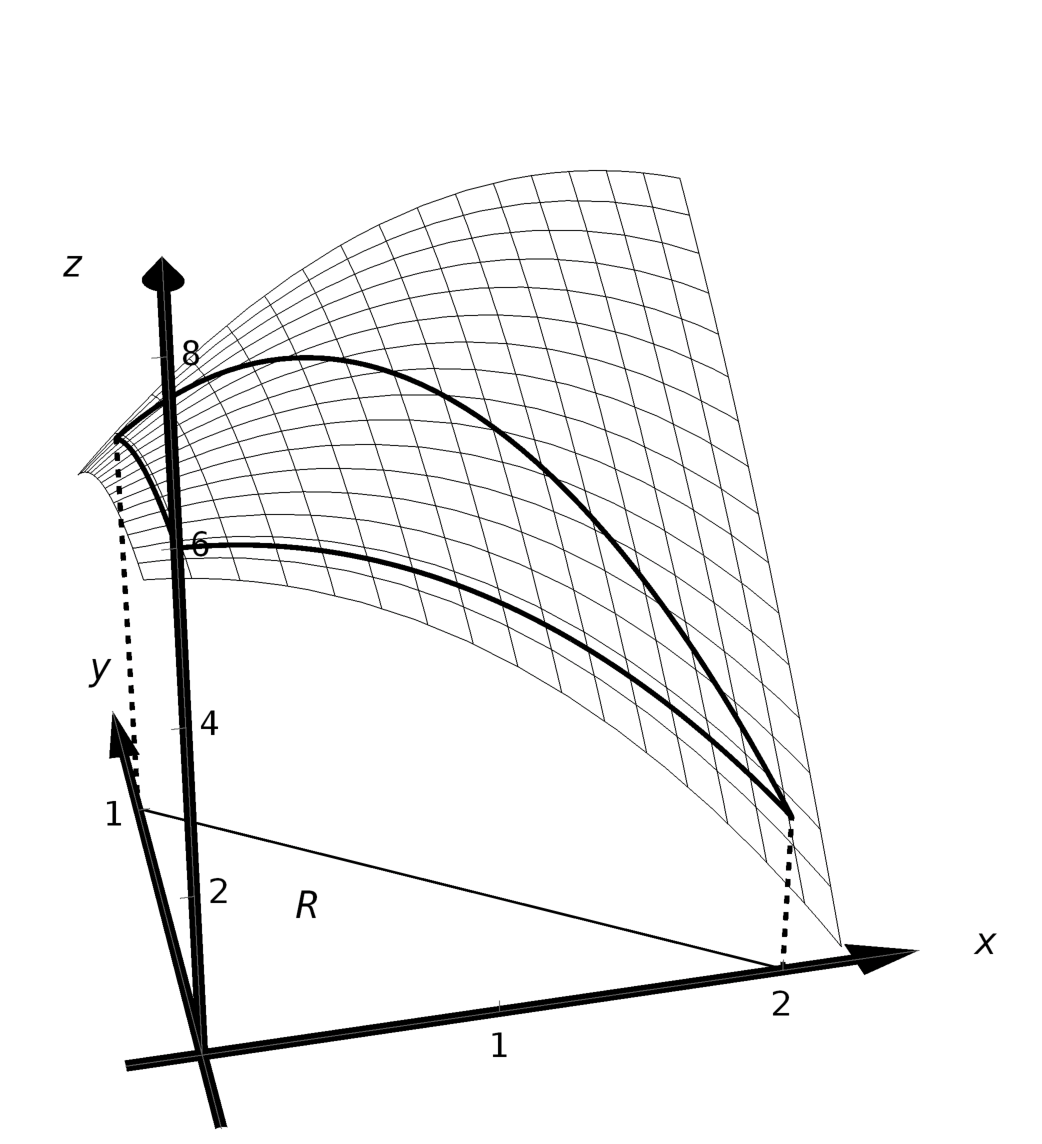
\includegraphics[width=0.5\textwidth]{fig_multiple_8}
	\caption{Finding the signed volume under a surface in Example \ref{ex_double2}.}
	\label{fig_multiple_8}
	\end{center}
\end{figure}


\xhrulefill{gray}{2.5pt}Solution \xhrulefill{gray}{2.5pt}

While it is not specified which order we are to use, we will evaluate the double integral using both orders to help drive home the point that it does not matter which order we use.\\


Using the order $dy\ dx$:
The bounds on $y$ go from curve to curve, i.e., $0\leq y\leq 1-x/2$, and the bounds on $x$ go from point to point, i.e., $0\leq x\leq 2$.
\allowdisplaybreaks
\begin{align*}
\iint_R (3xy-x^2-y^2+6\big)\ dA &= \int\limits_0^2\int\limits_0^{-\frac x2+1} (3xy-x^2-y^2+6\big)\ dy\ dx\\
		&= \int\limits_0^2 \left.\left(\frac32xy^2-x^2y-\frac13y^3+6y\right)\right|_0^{-\frac x2+1} dx\\
		&= \int\limits_0^2 \left(\frac{11}{12}x^3-\frac{11}{4}x^2-x+\frac{17}3\right)\ dx \\
		&= \left.\left(\frac{11}{48}x^4-\frac{11}{12}x^3-\frac12x^2+\frac{17}3x\right)\right|_0^2\\
		&= \frac{17}3\approx5.6.
\end{align*}

Now lets consider the order $dx \ dy$. Here $x$ goes from curve to curve, $0\leq x\leq 2-2y$, and $y$ goes from point to point, $0\leq y\leq 1$:
\begin{align*}
\iint_R (3xy-x^2-y^2+6\big)\ dA &= \int\limits_0^1\int\limits_0^{2-2y} (3xy-x^2-y^2+6\big)\ dx\ dy\\
		&= \int\limits_0^1 \left.\left(\frac32x^2y-\frac13x^3-xy^2+6x\right) \right|_0^{2-2y} dy\\
		&= \int\limits_0^1\left(\frac{32}3y^3-22y^2+2y+\frac{28}3\right)\ dy\\
		&=\left.\left(\frac83y^4-\frac{22}3y^3+y^2+\frac{28}3y\right)\right|_0^1\\
		&=\frac{17}3\approx5.6.
\end{align*}
We obtained the same result using both orders of integration. 
\end{example}

\subsection{Properties}

Note how in these two examples that the bounds of integration depend only on $R$; the bounds of integration have nothing to do with $f(x,y)$. Moreover, let $f$ and $g$ be continuous functions over a closed, bounded plane region $R$, and let $c$ be a constant, then we have the following properties, in line with the ones of single integrals. 

\begin{itemize}
	\item Constant multiple rule:
	$$\ds \iint_Rc\,f(x,y)\ dA = c\iint_Rf(x,y)\ dA.$$
	\item Sum/Difference rule:	
	$$\ds \iint_R \big(f(x,y)\pm g(x,y)\big)\ dA = \iint_R f(x,y)\ dA \pm \iint_R g(x,y)\ dA $$
	\item	If $f(x,y)\geq 0$ on $R$, then $$\ds \iint_R f(x,y)\ dA\geq 0.$$
	\item	If $f(x,y)\geq g(x,y)$ on $R$, then $$\ds \iint_R f(x,y)\ dA\geq \iint_R g(x,y)\ dA.$$
	\item Let $R$ be the union of two nonoverlapping regions, $R = R_1\cup R_2$. Then 
	$$\iint_R f(x,y)\ dA = \iint_{R_1}f(x,y)\ dA+ \iint_{R_2}f(x,y)\ dA.$$
\end{itemize}
Actually, since this property is intuitively clear, we relied already in Examples~\ref{ex_iterated5} and \ref{ex_double7}. Of course, this property generalizes to $n$ nonoverlapping regions.


\begin{example}\label{ex_double3}
Let $f(x,y) = \sin(x)\cos(y)$ and $R$ be the triangle with vertices $(-1,0)$, $(1,0)$ and $(0,1)$ (see Figure \ref{fig_multiple_9}). Evaluate the double integral $\iint_Rf(x,y)\ dA$.

\begin{figure}[H]
	\begin{center}			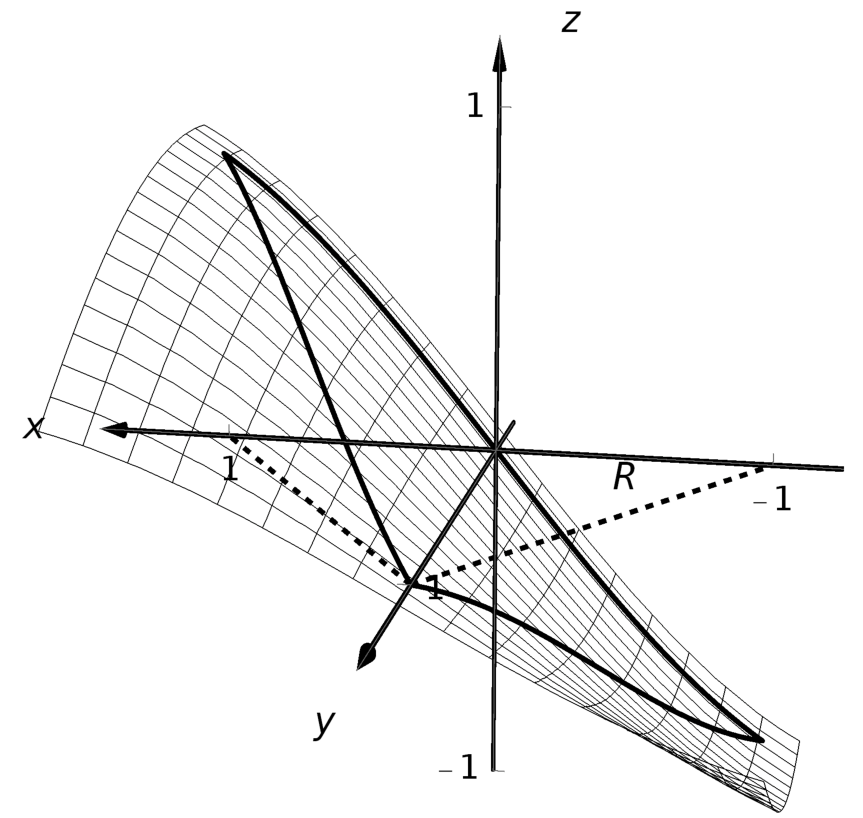
\includegraphics[width=0.5\textwidth]{fig_multiple_9}
	\caption{Finding the signed volume under a surface in Example \ref{ex_double3}.}
	\label{fig_multiple_9}
	\end{center}
\end{figure}


\xhrulefill{gray}{2.5pt}Solution \xhrulefill{gray}{2.5pt}


If we attempt to integrate using an iterated integral with the order $dy\ dx$, note how there are two upper bounds on $R$ meaning we will need to use two iterated integrals. We would need to split the triangle into two regions along the $y$-axis.

Instead, let us use the order $dx\ dy$. The curves bounding $x$ are $y-1\leq x\leq 1-y$; the bounds on $y$ are $0\leq y\leq 1$. This gives us:
\allowdisplaybreaks
\begin{align*}
\iint_R f(x,y)\ dA &= \int\limits_0^1\int\limits_{y-1}^{1-y}\sin(x)\cos(y)\ dx\ dy\\
		&= \int\limits_0^1\left.\Big( -\cos(x)\cos(y)\Big)\right|_{y-1}^{1-y} dy\\
		&= \int\limits_0^1 \cos(y)\Big(-\cos(1-y) + \cos(y-1)\Big)\ dy.
\end{align*}
Recall that the cosine function is an even function; that is, $\cos(x) = \cos(-x)$. Therefore, from the last integral above, we have $\cos(y-1) = \cos(1-y)$. Thus the integrand simplifies to 0, and we have 
$$
\iint_R f(x,y)\ dA = \int\limits_0^1 0\ dy = 0.
$$
It turns out that over $R$, there is just as much volume above the $xy$-plane as below (look again at Figure \ref{fig_multiple_9}), giving a final signed volume of 0. 
\end{example}

In the previous section we practised changing the order of integration of a given iterated integral, where the region $R$ was not explicitly given. Changing the bounds of an integral is more than just an test of understanding. Rather, there are cases where integrating in one order is really hard, if not impossible, whereas integrating with the other order is feasible.

\begin{example}\label{ex_double6}
Rewrite the iterated integral 
$$\ds \int\limits_0^3\int\limits_y^3 e^{-x^2}\ dx\ dy$$
with the order $dy\ dx$. Comment on the feasibility to evaluate each integral.

\xhrulefill{gray}{2.5pt}Solution \xhrulefill{gray}{2.5pt}

Once again we make a sketch of the region over which we are integrating to facilitate changing the order. The bounds on $x$ are from $x=y$ to $x=3$; the bounds on $y$ are from $y=0$ to $y=3$. These curves are sketched in Figure \ref{fig_multiple_10a}, enclosing the region $R$.

To change the bounds, note that the curves bounding $y$ are $y=0$ up to $y=x$; the triangle is enclosed between $x=0$ and $x=3$. Thus the new bounds of integration are $0\leq y\leq x$ and $0\leq x\leq 3$, giving the iterated integral $$\ds \int\limits_0^3\int\limits_0^x e^{-x^2}\ dy\ dx.$$ How easy is it to evaluate each iterated integral? Consider the order of integrating $dx\ dy$, as given in the original problem. The first indefinite integral we need to evaluate is $\int\limits e^{-x^2}\ dx$; we have stated before  that this integral cannot be evaluated in terms of elementary functions. We are stuck.

Changing the order of integration makes a big difference here. In the second iterated integral, we are faced with $\int\limits e^{-x^2}\ dy$; integrating with respect to $y$ gives us $ye^{-x^2}+C$, and the first definite integral evaluates to 
$$\int\limits_0^x e^{-x^2}\ dy = xe^{-x^2}.$$
Thus 
$$\int\limits_0^3\int\limits_0^x e^{-x^2}\ dy\ dx = \int\limits_0^3 xe^{-x^2}\ dx.$$
This last integral is easy to evaluate with substitution, giving a final answer of $(1-e^{-9})/2\approx 0.5$. Figure \ref{fig_multiple_10b} shows the surface over $R$. In short, evaluating one iterated integral is impossible; the other iterated integral is relatively simple.

\begin{figure}[H]
\centering
%\raisebox{0.5cm}{
\subfigure[\label{fig_multiple_10a}]{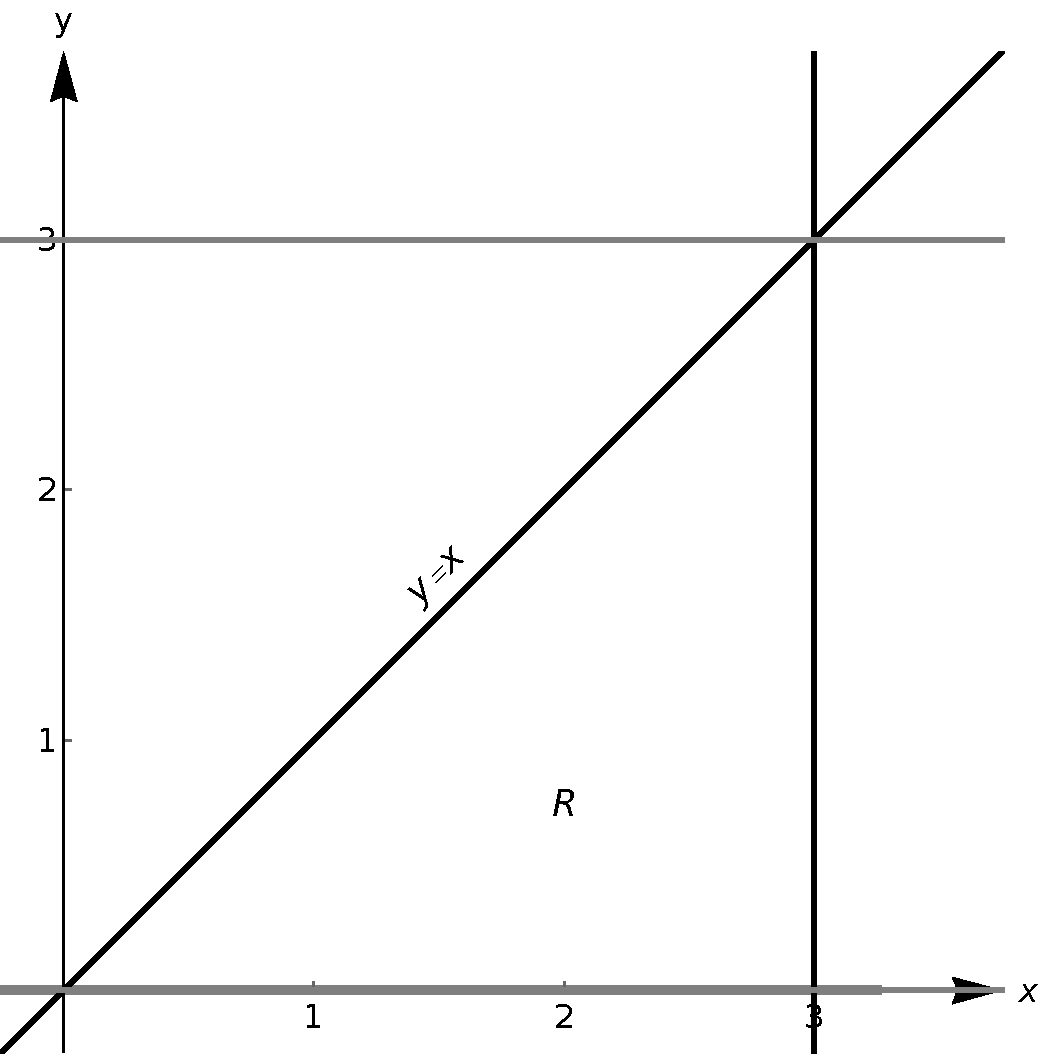
\includegraphics[width=0.43\textwidth]{fig_multiple_10a}}
\qquad
\subfigure[\label{fig_multiple_10b}]{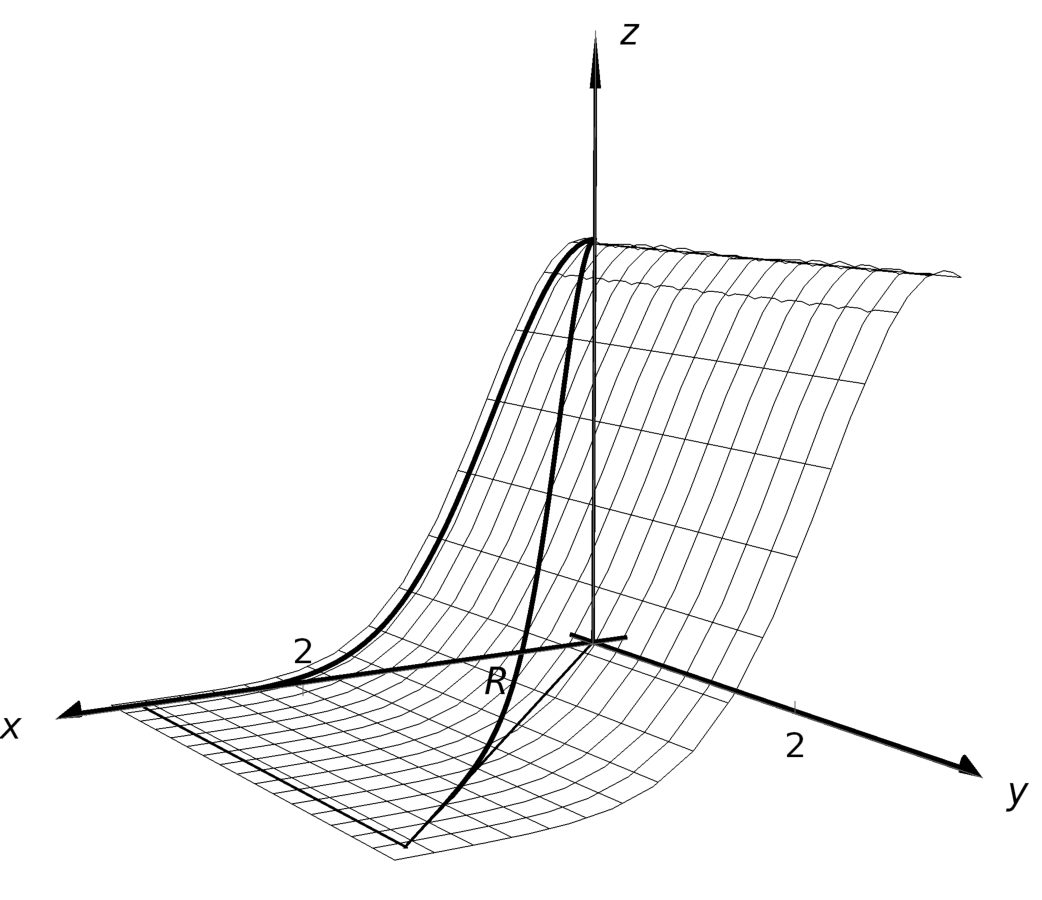
\includegraphics[width=0.43\textwidth]{fig_multiple_10b} }
\caption{Determining the region $R$ determined by the bounds of integration (a) and the surface $f$ over its region $R$ in Example \ref{ex_double6}.}
\end{figure}

\end{example}

	\checkoddpage
\marginpar{\ifoddpage\hspace*{-1.5cm}\else\hspace*{0.25cm}\fi
\includegraphics[width=0.075\textwidth]{youtube}\\
\ifoddpage\hspace*{-1.75cm}\else\hspace*{0.1cm}\fi
\qrcode[height=1.75cm]{https://youtu.be/dzuoNwC6ZeI}
%\includegraphics[width=0.1\textwidth]{mean_function_value_3d}
}

Using double integrals we can also determine the average value of $z=f(x,y)$ over a region $R$. This is nothing but the volume under $f$ over $R$ divided by the area of $R$; that is
\begin{equation}
\text{average value of $f$ on $R$} = \frac{\ds \iint_R f(x,y)\ dA}{\ds\iint_R \ dA}.
\label{def:av_val2}
\end{equation}


\begin{example}\label{ex_double8}
Find the average value of $f(x,y) = 4-y$ over the region $R$, which is bounded by the parabolas $y^2=4x$ and $x^2=4y$ (see Figure~\ref{fig_multiple_11}). 




\xhrulefill{gray}{2.5pt}Solution \xhrulefill{gray}{2.5pt}

Graphing each curve can help us find their points of intersection. Solving analytically, the second equation tells us that $y=x^2/4$. Substituting this value in for $y$ in the first equation gives us $x^4/16 = 4x$. Solving for $x$:

\allowdisplaybreaks
\begin{align*}
& \qquad \frac{x^4}{16} = 4x\\
\Leftrightarrow & \qquad x^4-64x = 0\\
\Leftrightarrow & \qquad x(x^3-64)  = 0\\
\Leftrightarrow & \qquad x = 0 \;  \vee \;  x = 4.
\end{align*}
Thus we have found analytically what was easy to approximate graphically: the regions intersect at $(0,0)$ and $(4,4)$, as shown in Figure \ref{fig_multiple_11}. 

\begin{figure}[H]
	\begin{center}
			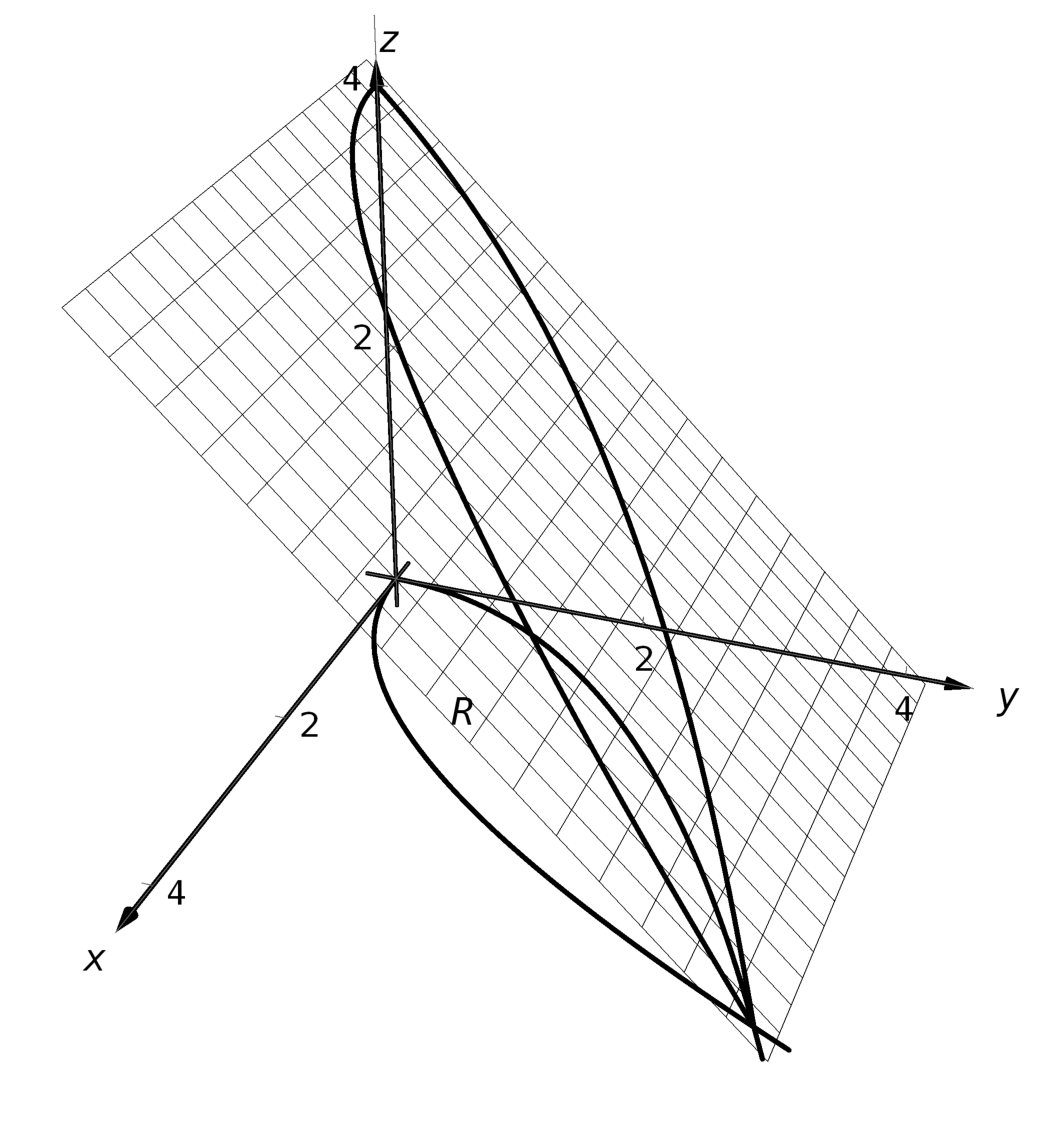
\includegraphics[width=0.5\textwidth]{fig_multiple_11}
	\caption{Finding the signed volume under a surface in Example \ref{ex_double8}.}
	\label{fig_multiple_11}
	\end{center}
\end{figure}

We now choose an order of integration: $dy\ dx$ or $dx\ dy$? Either order works; since the integrand does not contain $x$, choosing $dx\ dy$ might be simpler -- at least, the first integral is very simple.

Thus we have the following curve to curve, point to point bounds: $y^2/4\leq x\leq 2\sqrt y$, and $0\leq y\leq 4$. 
\begin{align*}
\iint_R (4-y)\ dA &= \int\limits_0^4\int\limits_{y^2/4}^{2\sqrt{y}}(4-y)\ dx\ dy\\
&= \int\limits_0^4(4-y)\int\limits_{y^2/4}^{2\sqrt{y}}\ dx\ dy\\
				&= \int\limits_0^4 \big(x(4-y)\big)\Big|_{y^2/4}^{2\sqrt{y}} dy\\
				&= \int\limits_0^4 \left[\left(2\sqrt{y}-\frac{y^2}{4}\right)(4-y)\right]\ dy = \int\limits_0^4 \Big( \frac{y^3}{4}-y^2-2y^{3/2}+8y^{1/2}\Big)\ dy\\
				&= \left.\left(\frac{y^4}{16}-\frac{y^3}{3}-\frac{4y^{5/2}}5+\frac{16y^{3/2}}3\right)\right|_0^4\\
				&= \frac{176}{15} \approx 11.73.
\end{align*}



We now find the area of $R$ by computing $\iint_R \ dA$:
$$\iint_R \ dA = \int\limits_0^4\int\limits_{y^2/4}^{2\sqrt{y}} \ dx\ dy = \frac{16}{3}.$$
Dividing the volume under the surface by the area gives the average value:
$$\text{average value of $f$ on $R$} = \frac{176/15}{16/3} = \frac{11}5 = 2.2.$$
While the surface covers $z$-values from $z=0$ to $z=4$, the average $z$-value on $R$ is 2.2.
\end{example}

Our new understanding of double integrals allows us to revisit what we did in the previous section. Given a region $R$ in the plane, we computed $\iint_R 1\ dA$; again. Our understanding at the time was that we were finding the area of $R$. However, we can now view the function $z=1$ as a surface, a flat surface with constant $z$-value of 1. The double integral $\iint_R 1\ dA$ finds the volume, under $z=1$, over $R$. We were actually computing the volume of a solid, though we interpreted the number as an area.



\subsection{Differentiation under the integral sign}\label{sec:afl_Leibniz}
Sometimes we will run into the derivative of an integral of a function of two variables, where, however, one of the variables is considered as a parameter. For instance, we may encounter something like 
$$
\displaystyle \int\limits_{a(x)}^{b(x)}f(x,t)\,dt\,,
$$
where $ -\infty <a(x),b(x)<+\infty$. Even though the way how to proceed with this is very intuitive, the formal proof is rather involved, especially for the general case with variable limits. We first state the result as a theorem. 

\begin{theorem}[Leibniz integral rule]
\label{thm:leibniz}
Let $f(x, t)$ be a function such that both $f(x, t)$ and its partial derivative $f_x(x, t)$ are continuous in some region of the $xt$-plane, including $a(x) \leq t\leq b(x), x_0 \leq x \leq x_1$. Also suppose that the functions $a(x)$ and $b(x)$ are both continuous and both have continuous derivatives for $x_0 \leq x \leq x_1$. Then, for $x_0 \leq x \leq x_1$, we have that
$$\displaystyle {\frac {d}{dx}}\left(\int\limits _{a(x)}^{b(x)}f(x,t)\,dt\right)=f{\big (}x,b(x){\big )} {\frac {d}{dx}}b(x)-f{\big (}x,a(x){\big )} {\frac {d}{dx}}a(x)+\int\limits _{a(x)}^{b(x)}{\frac {\partial }{\partial x}}f(x,t)\,dt\,.
$$
\end{theorem}
\begin{proof}
The general form of this theorem can be derived as a consequence of the basic form of leibniz's integral rule with constant limits of integration, the multivariable chain rule, and the fundamental theorem of calculus. So, let us first prove the simpler case with constant limits of integration, i.e.
$$
\displaystyle {\frac {d}{dx}}\left(\int\limits _{a}^{b}f(x,t)\,dt\right)=\int\limits _{a}^{b}{\frac {\partial }{\partial x}}f(x,t)\,dt.
$$
Essentially, in an attempt to get a derivative in the right-hand side of the above equation, as is the case in its left-hand side, we may rewrite it according to the fundamental theorem of calculus (Section~\ref{sec:FTC}) as
$$
\dfrac{d}{dx}\left(\int\limits_A^x \left( \int\limits _{a}^{b}{\frac {\partial }{\partial s}}f(s,t)\,dt\right) ds\right)\,,
$$
because we have function of one variable $s$ within the inner parentheses. Subsequently, we rely on Fubini's theorem to interchange the order of integration
\begin{eqnarray*}
\dfrac{d}{dx}\left(\int\limits_A^x \left( \int\limits _{a}^{b}{\frac {\partial }{\partial s}}f(s,t)\,dt\right) ds\right)&=&\dfrac{d}{dx}\left(\int\limits_a^b \left( \int\limits_{A}^{x}{\frac {\partial }{\partial s}}f(s,t)\ ds\right)dt\right)\,,\\[0.2cm]
&=&\dfrac{d}{dx}\int\limits_a^b   \left(f(x,t)-f(A,t)\right)\ dt\,,\\[0.2cm]
&=&\dfrac{d}{dx}\int\limits_a^b   f(x,t)\ dt-\dfrac{d}{dx}\int\limits_a^b   f(A,t)\ dt\,,\\[0.2cm]
&=&\dfrac{d}{dx}\int\limits_a^b  f(x,t)\ dt\,,\\[0.2cm]
\end{eqnarray*}

To prove the general case with variable limits, suppose now $f$ is defined in a rectangle in the $xt$-plane, for $x\in [x_{0},x_{1}]$ and $t\in [t_{0},t_{1}]$. Also, assume $f$ and the partial derivative $f_x$ are both continuous functions on this rectangle. Suppose $a,\,b$ are differentiable real valued functions defined on $[x_{0},x_{1}]$ with values in $[t_{0},t_{1}]$ (i.e for every $\displaystyle x\in [x_{0},x_{1}],a(x),b(x)\in [t_{0},t_{1}]$). Now, set
$$
\displaystyle F(x,y)=\int\limits _{t_{0}}^{y}f(x,t)\,dt
$$
for $x\in [x_{0},x_{1}]$ and $y\in [t_{0},t_{1}]$ and
$$
\displaystyle G(x)=\int\limits _{a(x)}^{b(x)}f(x,t)\,dt
$$ for $x\in [x_{0},x_{1}]$. Then, by properties of definite integrals, we can write
$$
\displaystyle {\begin{aligned}G(x)&=\int\limits _{t_{0}}^{b(x)}f(x,t)\,dt-\int\limits _{t_{0}}^{a(x)}f(x,t)\,dt\\&=F(x,b(x))-F(x,a(x)).\end{aligned}}
$$
Since the partial derivatives of $F$ are given by $$\dfrac{\partial F}{\partial x}(x,y)=\int _{t_{0}}^{y}{\dfrac {\partial f}{\partial x}}(x,t)dt$$ and $$\dfrac {\partial F}{\partial y}(x,y)=f(x,y)$$ and recalling $f_x$ is continuous, its integral is also a continuous function. Moreover,  since $f$ is also continuous, these two results show that both  partial derivatives of $F$  are continuous. Since continuity of partial derivatives implies differentiability of the function, $F$ is  differentiable. So, since the functions $F,\,a,\,b$ are all differentiable, by the multivariable chain rule, it follows that $G$ is differentiable, and its derivative is given by the formula:
$$
\displaystyle G'(x)=\left({\dfrac {\partial F}{\partial x}}\left(x,b(x)\right)+{\dfrac {\partial F}{\partial y}}\left(x,b(x)\right)b'(x)\right)-\left({\dfrac {\partial F}{\partial x}}\left(x,a(x)\right)+{\dfrac {\partial F}{\partial y}}\left(x,a(x)\right)a'(x)\right)\,.
$$
Now, note that for every $x\in [x_{0},x_{1}]$, and for every $y\in [t_{0},t_{1}]$, we have that 
$$\displaystyle {\dfrac {\partial F}{\partial x}}(x,y)=\int\limits _{t_{0}}^{y}{\dfrac {\partial f}{\partial x}}(x,t)dt\, ;$$ because when taking the partial derivative with respect to $x$ of $F$, we are keeping $y$  fixed in the expression 
$$
\displaystyle \int\limits _{t_{0}}^{y}f(x,t)\,dt\,.
$$
Consequently, the basic form of Leibniz's integral rule with constant limits of integration applies. Next, by the first fundamental theorem of calculus, we have that $$\displaystyle {\dfrac {\partial F}{\partial y}}(x,y)=f(x,y)\,;$$ because when taking the partial derivative with respect to $y$ of $F$, the first variable $x$ is fixed, so the fundamental theorem can indeed be applied. Substituting these results into the equation for $G'(x)$ above gives:
$$
\displaystyle {\begin{aligned}G'(x)&=\left(\int\limits _{t_{0}}^{b(x)}{\dfrac {\partial f}{\partial x}}(x,t)dt+f\left(x,b(x)\right)b'(x)\right)-\left(\int\limits _{t_{0}}^{a(x)}{\dfrac {\partial f}{\partial x}}(x,t)dt+f\left(x,a(x)\right)a'(x)\right)\\[0.2cm]
&=f\left(x,b(x)\right)b'(x)-f\left(x,a(x)\right)a'(x)+\int\limits _{a(x)}^{b(x)}{\dfrac {\partial f}{\partial x}}(x,t)dt,\end{aligned}}
$$
as desired. 
\end{proof}

\pagebreak
\begin{example}
Using Leibniz integral rule, we easily find that, for instance,
$$
\allowdisplaybreaks
\begin{aligned}{\frac {d}{dx}}\left(\int\limits _{\sin (x)}^{\cos (x)}\cosh (t^{2})\,dt\right)&=\cosh \left(\cos ^{2}(x)\right){\frac {d}{dx}}(\cos (x))-\cosh \left(\sin ^{2}(x)\right){\frac {d}{dx}}(\sin (x))+\int\limits _{\sin (x)}^{\cos (x)}{\frac {\partial }{\partial x}}\left(\cosh (t^{2})\right)dt\\&=\cosh \left(\cos ^{2}(x)\right)(-\sin (x))-\cosh \left(\sin ^{2}(x)\right)(\cos (x))+0\\&=-\cosh \left(\cos ^{2}(x)\right)\sin (x)-\cosh \left(\sin ^{2}(x)\right)\cos (x).\end{aligned}
$$
Still, the principle of differentiating under the integral sign is typically used to evaluate a definite integral in cases where one cannot easily find an antiderivative.
\end{example}


% voorbeeld: https://brilliant.org/wiki/differentiate-through-the-integral/

\begin{example}
Compute the definite integral
$$
\int\limits_0^1\dfrac{t^3-1}{\ln(t)}\ dt\,.
$$

\xhrulefill{gray}{2.5pt}Solution \xhrulefill{gray}{2.5pt}


This integral appears resistant to standard integration techniques such as integration by parts, substitution, and so on. Hence, we would like to use differentiation under the integral sign to compute it. But how can we choose a function to differentiate under the integral sign? The appearance of $\ln(t)$ in the denominator of the integrand is of course quite unwelcome, and we would like to get rid of it. Luckily, we know 
$$
\dfrac{d(t^x)}{dx}=t^x\ln(t)
$$
so differentiating the numerator with respect to the exponent seems to be what we would like to do. Accordingly, we define a function 
$$
g(x)=\int\limits_0^1\dfrac{t^x-1}{\ln(t)}\ dt\,.
$$
In this notation, the integral we wish to evaluate is $g(3)$. Observe that the given integral has been recast as member of a family of definite integrals indexed by the variable $x$.

By Leibniz integral rule, we compute 
$$
\dfrac{dg(x)}{dx}=\int\limits_0^1\dfrac{\partial}{\partial x}\left(\dfrac{t^x-1}{\ln(t)}\right)\ dt=\int\limits_0^1\dfrac{t^x\ln(t)}{\ln(t)}\ dt=\left.\dfrac{t^{x+1}}{x+1}\right|_0^1=\dfrac{1}{x+1}\,.
$$
It follows that $g(x)=\ln|x+1|+C$ for some constant $C$. To determine this constant $C$, note that $g(0)=0$, so $g(0)=0=\ln|1|+C$, from which we conclude that $C=0$. Hence, $g(x)=\ln|x+1|$ for all $x$ such that the integral exists. In particular,  $g(3)=\ln(4)$.
\end{example}


\subsection{Double integration with polar coordinates}
\label{sec:double_int_polar}
Some regions $R$ are easy to describe using rectangular coordinates -- that is, with equations of the form $y=f(x)$, $x=a$, etc. However, some regions are easier to handle if we represent their boundaries with polar equations of the form $r=f(\theta)$, $\theta = \alpha$, etc. 

The basic form of the double integral is $\iint_R f(x,y)\ dA$. We interpret this integral as follows: over the region $R$, sum up lots of products of heights (given by $f(x_i,y_i)$) and areas (given by $\Delta A_i$). That is, $dA$ represents a little bit of area. In rectangular coordinates, we can describe a small rectangle as having area $dx\ dy$ or $dy\ dx$ -- the area of a rectangle is simply (length$\times$width) -- a small change in $x$ times a small change in $y$. Thus we replace $dA$ in the double integral with $dx\ dy$ or $dy\ dx$.

Now consider representing a region $R$ with polar coordinates. Consider Figure \ref{fig_multiple_12a}. Let $R$ be the region in the first quadrant bounded by the curve. We can approximate this region using the natural shape of polar coordinates: portions of sectors of circles. In the figure, one such region is shaded, shown again in Figure~\ref{fig_multiple_12b}.

\begin{figure}
\centering
%\raisebox{0.5cm}{
\subfigure[\label{fig_multiple_12a}]{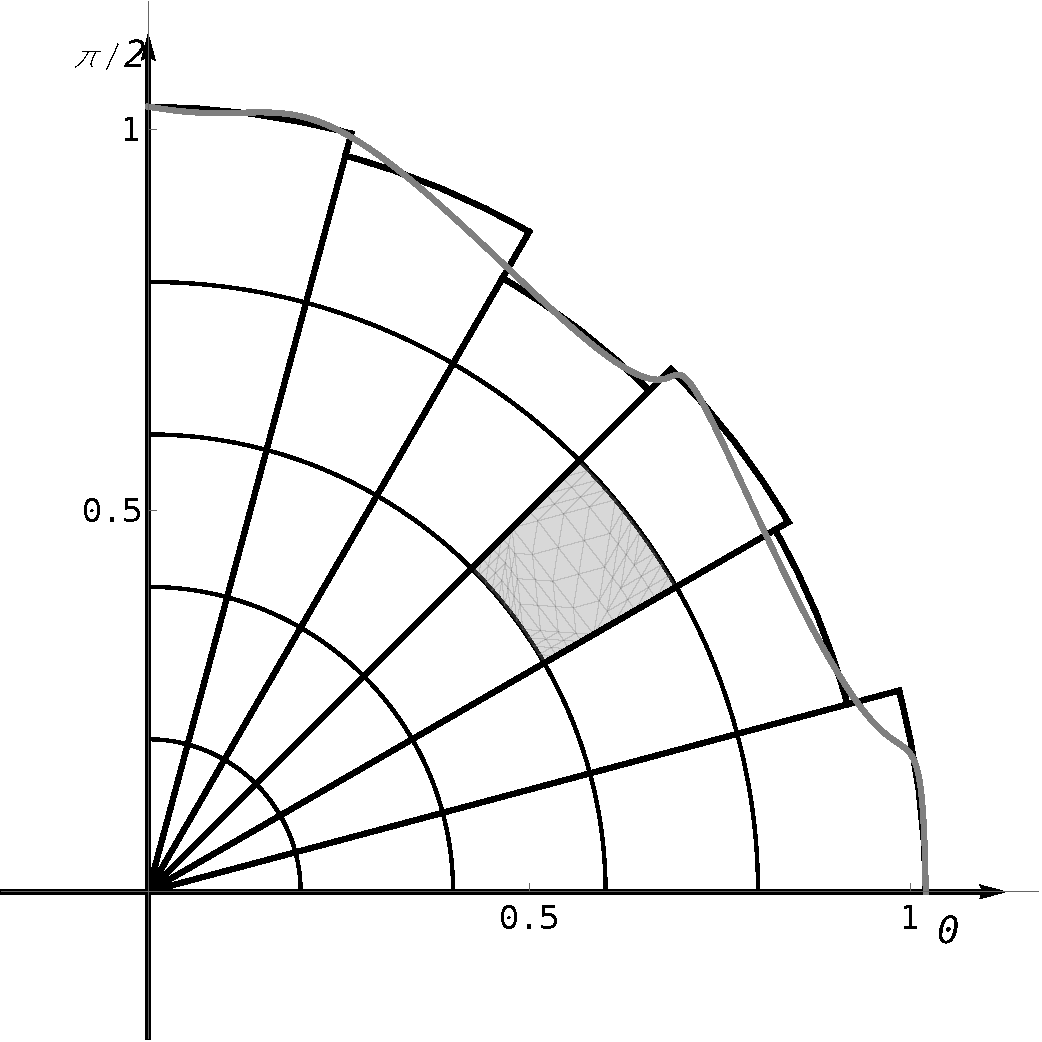
\includegraphics[width=0.43\textwidth]{fig_multiple_12a}}
\qquad
\subfigure[\label{fig_multiple_12b}]{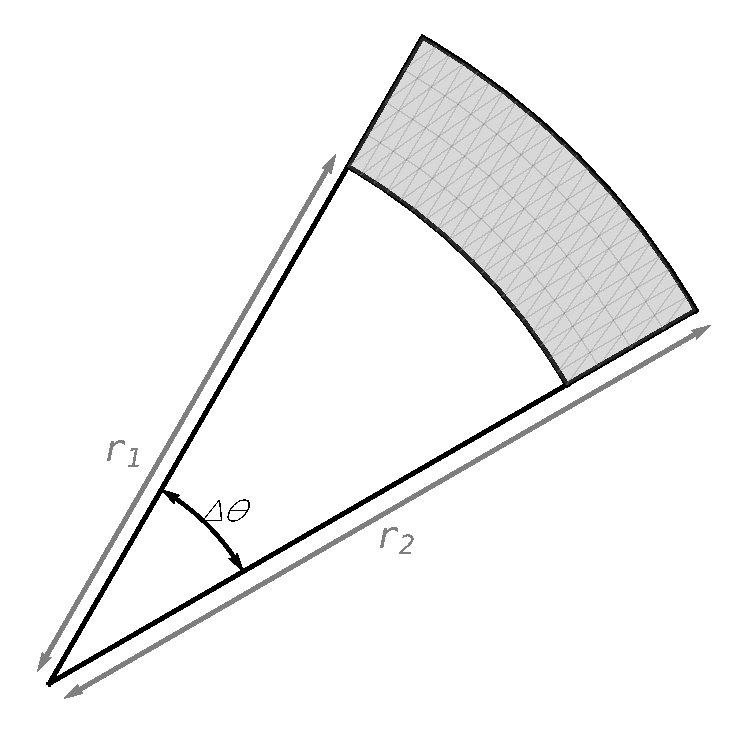
\includegraphics[width=0.43\textwidth]{fig_multiple_12b} }
\caption{Approximating a region $R$ with portions of sectors of circles.}
\end{figure}

As the area of a sector of a circle with radius $r$, subtended by an angle $\theta$, is $A = \frac12r^2\theta$, we can find the area of the shaded region. The whole sector has area $\frac12r_2^2\Delta \theta$, whereas the smaller, unshaded sector has area $\frac12r_1^2\Delta \theta$. The area of the shaded region is the difference of these areas:
$$\Delta A_i = \frac12r_2^2\Delta\theta-\frac12r_1^2\Delta\theta = \frac12\big(r_2^2-r_1^2\big) \Delta\theta = \frac{r_2+r_1}{2}\big(r_2-r_1\big) \Delta\theta.$$

Note that $(r_2+r_1)/2$ is just the average of the two radii. 

To approximate the region $R$, we use many such subregions; doing so shrinks the difference $r_2-r_1$ between radii to 0 and shrinks the change in angle $\Delta \theta$ also to 0. We represent these infinitesimal changes in radius and angle as $dr$ and $d\theta$, respectively. Finally, as $dr$ is small, $r_2\approx r_1$, and so \\ $(r_2+r_1)/2\approx r_1$. Thus, when $dr$ and $d\theta$ are small, 
$$\Delta A_i \approx r_i\ dr\ d\theta.$$

Taking a limit, where the number of subregions goes to infinity and both $r_2-r_1$ and $\Delta\theta$ go to 0, we get $$dA = r\ dr\ d\theta.$$

So to evaluate $\iint_Rf(x,y)\ dA$, replace $dA$ with $r\ dr\ d\theta$. Convert the function $z=f(x,y)$ to a function with polar coordinates with the substitutions $x=r\cos(\theta)$, $y=r\sin(\theta)$. Finally, find bounds $g_1(\theta)\leq r\leq g_2(\theta)$ and $\alpha\leq\theta\leq\beta$ that describe $R$. Consequently, if $z=f(x,y)$ is a continuous function defined over a closed, bounded region $R$ in the $xy$-plane, where $R$ is
%Let $R$ be a plane region 
bounded by the polar equations $\alpha\leq\theta\leq\beta$ and  $g_1(\theta)\leq r\leq g_2(\theta)$, then 
\begin{equation}
\iint_Rf(x,y)\ dA = \int\limits_\alpha^\beta\int\limits_{g_1(\theta)}^{g_2(\theta)} f\big(r\cos(\theta),r\sin(\theta)\big)\ r\ dr\ d\theta.
\label{idea:doublepol}
\end{equation}

Examples will help us understand this.


\pagebreak
\begin{example}\label{ex_doublepol1}
Find the signed volume under the plane $z= 4-x-2y$ over the disk bounded by the circle with equation $x^2+y^2=1$.

\xhrulefill{gray}{2.5pt}Solution \xhrulefill{gray}{2.5pt}

The bounds of the integral are determined solely by the region $R$ over which we are integrating. In this case, it is a disk with boundary $x^2+y^2=1$. We need to find polar bounds for this region. Bounds for this disk are $0\leq r\leq 1$ and $0\leq \theta\leq 2\pi$.

We replace $f(x,y)$ with $f\left(r\cos(\theta),r\sin(\theta)\right)$. That means we make the following substitutions:
$$4-x-2y \quad \Rightarrow \quad 4-r\cos(\theta)-2r\sin(\theta).$$
Finally, we replace $dA$ in the double integral with $r\ dr\ d\theta$. This gives the final iterated integral, which we evaluate:
\allowdisplaybreaks
\begin{align*}
\iint_Rf(x,y)\ dA &= \int\limits_0^{2\pi}\int\limits_0^1\big(4-r\cos(\theta)-2r\sin(\theta)\big)r\ dr\ d\theta\\
						&= \int\limits_0^{2\pi}\int\limits_0^1\Big(4r-r^2\big(\cos(\theta)-2\sin(\theta)\big)\Big)\ dr\ d\theta\\
						&= \int\limits_0^{2\pi}\left.\left(2r^2-\frac13r^3\big(\cos(\theta)-2\sin(\theta)\big)\right)\right|_0^1d\theta\\
						&= \int\limits_0^{2\pi} \left(2-\frac13\big(\cos(\theta)-2\sin(\theta)\big)\right)\ d\theta\\
						&= \left.\left(2\theta -\frac13\big(\sin(\theta)+2\cos(\theta)\big)\right)\right|_0^{2\pi} \\
						&= 4\pi \approx 12.566.
\end{align*}
The surface and region $R$ are shown in Figure \ref{fig_multiple_13}.

\begin{figure}[H]
	\begin{center}
			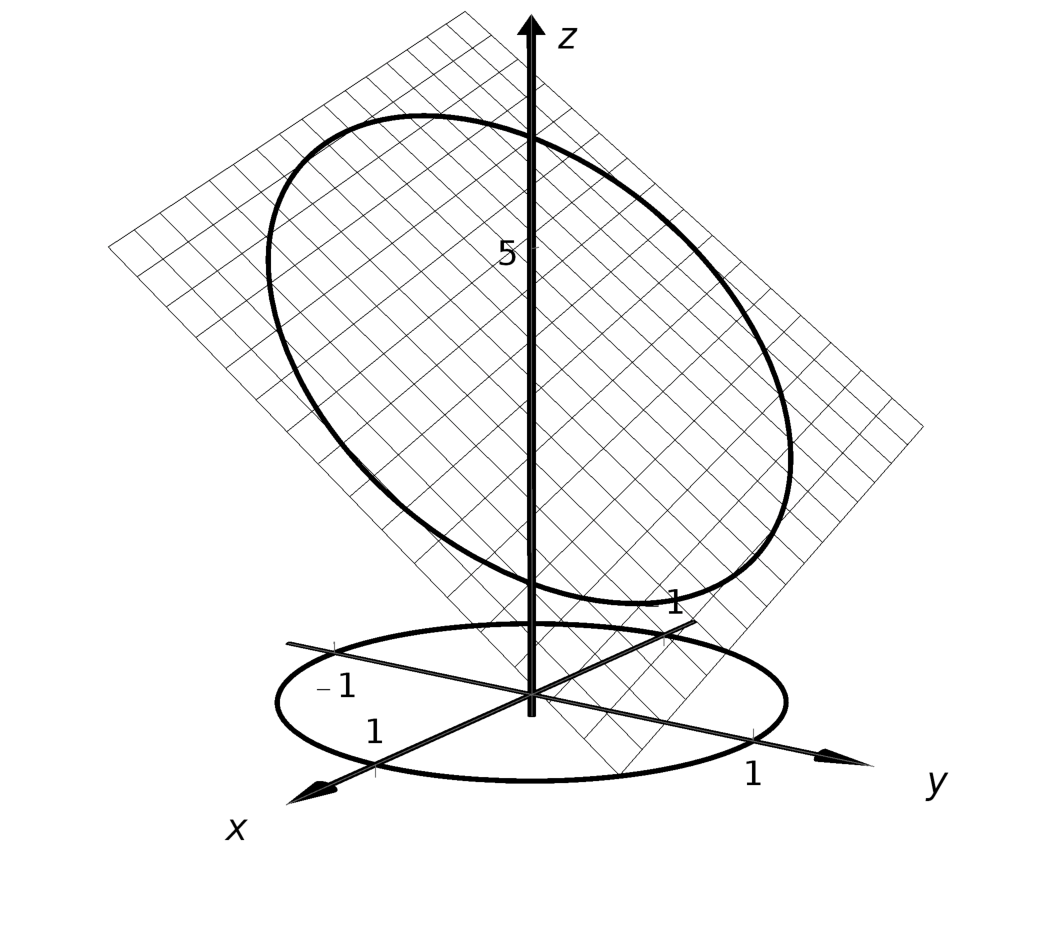
\includegraphics[width=0.4\textwidth]{fig_multiple_13}
	\caption{Evaluating a double integral with polar coordinates in Example \ref{ex_doublepol1}.}
	\label{fig_multiple_13}
	\end{center}
\end{figure}

\end{example}

\begin{example}\label{ex_doublepol2}
Find the volume under the paraboloid $z=4-(x-2)^2-y^2$ over the region bounded by the circles $(x-1)^2+y^2=1$ and $(x-2)^2+y^2=4$.

\xhrulefill{gray}{2.5pt}Solution \xhrulefill{gray}{2.5pt}

At first glance, this seems like a very hard volume to compute as the region $R$ (shown in Figure \ref{fig_multiple_14a}) has a hole in it, cutting out a strange portion of the surface, as shown in Figure~\ref{fig_multiple_14b}. However, by describing $R$ in terms of polar equations, the volume is not very difficult to compute.


\begin{figure}[H]
\centering
%\raisebox{0.5cm}{
\subfigure[\label{fig_multiple_14a}]{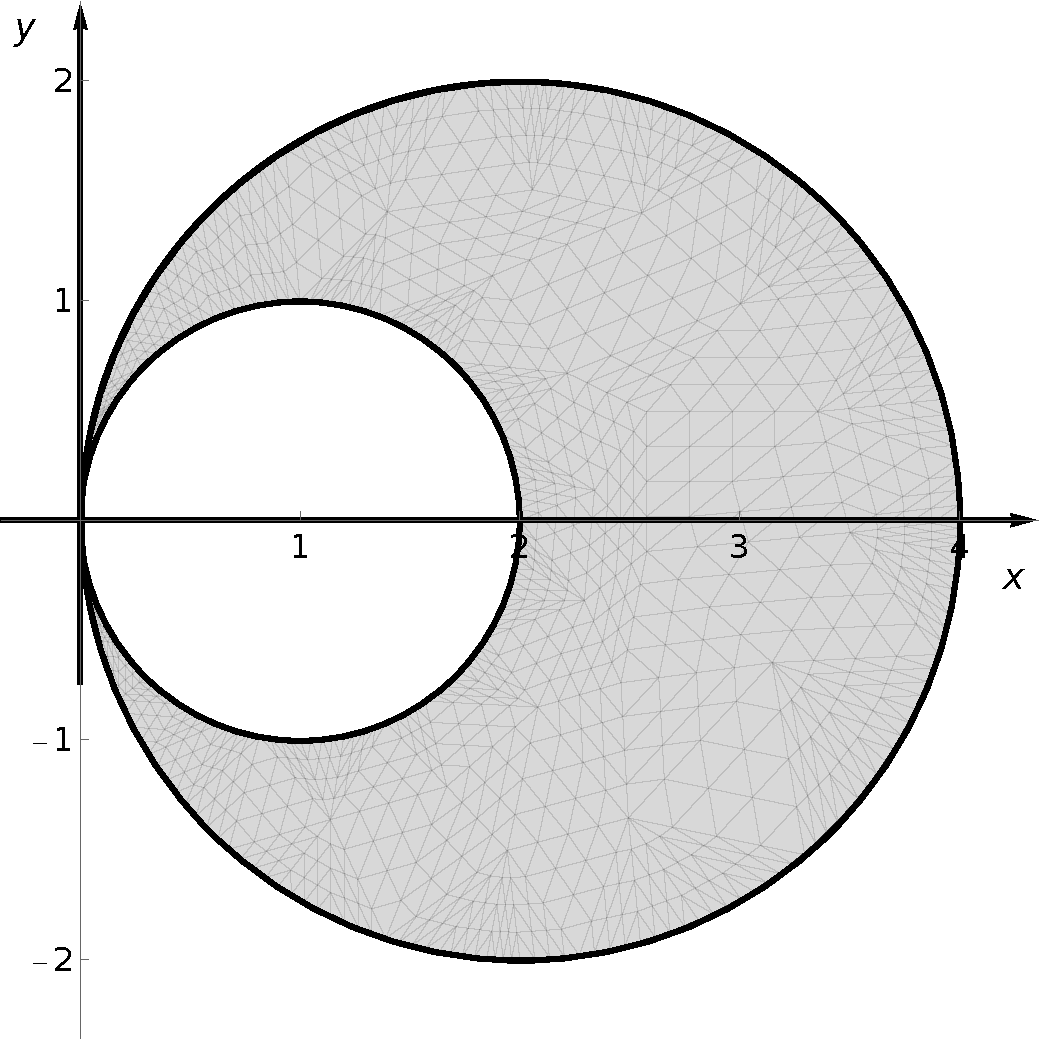
\includegraphics[width=0.43\textwidth]{fig_multiple_14a}}
\qquad
\subfigure[\label{fig_multiple_14b}]{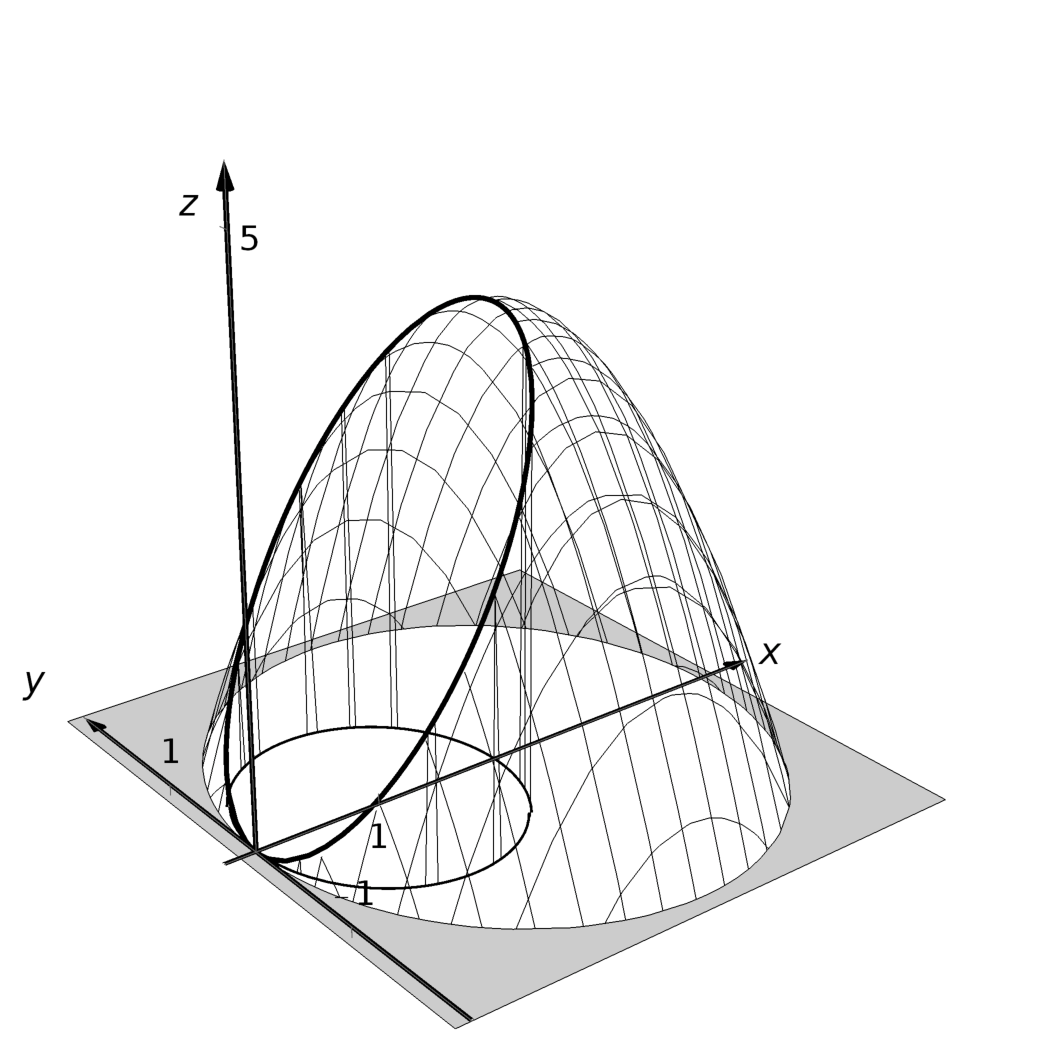
\includegraphics[width=0.43\textwidth]{fig_multiple_14b} }
\caption{Showing the region $R$ (a) and surface (b) used in Example \ref{ex_doublepol2}}
\end{figure}



The circle $(x-1)^2+y^2=1$ has polar equation $r=2\cos(\theta)$, while the circle $(x-2)^2+y^2=4$ has polar equation $r=4\cos(\theta)$. We may trace out semicircles on the interval $0\leq\theta\leq\pi/2$. The bounds on $r$ are $2\cos(\theta)\leq r\leq 4\cos(\theta).$ Replacing $x$ with $r\cos(\theta)$ in the integrand, along with replacing $y$ with $r\sin(\theta)$ and noting that we should add a factor 2 to account for the entire volume, prepares us to evaluate the double integral $\iint_Rf(x,y)\ dA$:

\allowdisplaybreaks
\begin{align*}
\iint_Rf(x,y)\ dA &=2 \int\limits_0^{\pi/2}\int\limits_{2\cos(\theta)}^{4\cos(\theta)} \Big(4-\big(r\cos(\theta)-2\big)^2-\big(r\sin(\theta)\big)^2\Big)r\ dr\ d\theta\\
			%&=\int\limits_0^{\pi}\int\limits_{2\cos\theta}^{4\cos\theta} \big(r^3\cos^2\theta + r^3\sin^2\theta -4r^2\cos \theta+4r\big)\ dr\ d\theta\\
			&= 2\int\limits_0^{\pi/2}\int\limits_{2\cos(\theta)}^{4\cos(\theta)} \big(-r^3+4r^2\cos(\theta)\big)\ dr\ d\theta\\
			&= 2\int\limits_0^{\pi/2} \left.\left(-\frac14r^4+\frac43r^3\cos(\theta)\right)\right|_{2\cos(\theta)}^{4\cos(\theta)}d\theta\\
			&=2\int\limits_0^{\pi/2} \left(\left[-\frac14\Big(256\cos^4(\theta)\Big)+\frac43\Big(64\cos^4(\theta)\Big)\right]-\right.\\
			&\ \quad\quad\quad\left.\left[-\frac14\Big(16\cos^4(\theta)\Big)+\frac43\Big(8\cos^4(\theta)\Big)\right]\right)\ d\theta\\
			&=2\int\limits_0^{\pi/2}\frac{44}3\cos^4(\theta)\ d\theta.
\intertext{To integrate $\cos^4(\theta)$, rewrite it as $\cos^2(\theta)\cos^2(\theta)$ and employ the power-reducing formula twice:}
	\cos^4(\theta) &=\cos^2(\theta)\cos^2(\theta)\\
								&= \frac12\big(1+\cos(2\theta)\big)\frac12\big(1+\cos(2\theta)\big) \\
								&= \frac14\big(1+2\cos(2\theta)+\cos^2(2\theta)\big)\\
								&=\frac14\Big(1+2\cos(2\theta)+\frac12\big(1+\cos(4\theta)\big)\Big)\\
								&= \frac38+\frac12\cos(2\theta)+\frac18\cos(4\theta).
		\intertext{Picking up from where we left off above, we have}
\iint_Rf(x,y)\ dA &=2\int\limits_0^{\pi/2}\frac{44}3\cos^4(\theta)\ d\theta\\
		&=2\int\limits_0^{\pi/2} \frac{44}3\left(\frac38+\frac12\cos(2\theta)+\frac18\cos(4\theta)\right)d\theta\\
		&= \left.\frac{88}3\left(\frac{3}8\theta+\frac14\sin(2\theta)+\frac{1}{32}\sin(4\theta)\right)\right|_0^{\pi/2}\\
		&=\frac{11}2\pi\approx 17.279.
\end{align*}
Note that the double integral would have been much harder to evaluate had we used rectangular coordinates.
\end{example}


\ifanalysis
\begin{example}\label{ex_doublepol5}

Find the volume under the surface $\ds f(x,y) =\left(x^2+y^2+1\right)^{-1}$ over the  sector of the circle with radius $a$ centered at the origin in the first quadrant, as shown in Figure \ref{fig_multiple_15}.

\begin{figure}[H]
	\begin{center}
			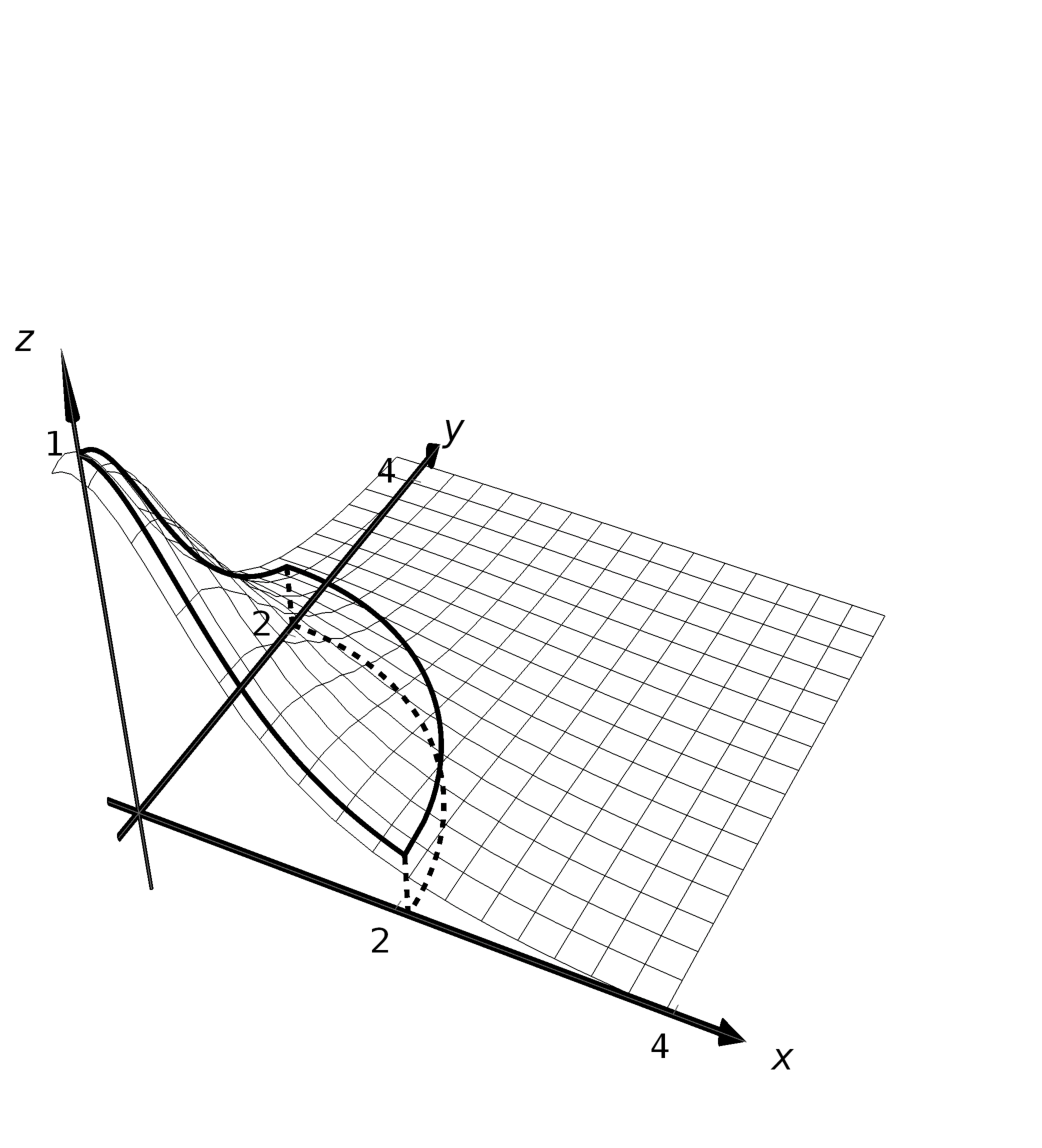
\includegraphics[width=0.5\textwidth]{fig_multiple_15}
	\caption{The surface and region $R$ used in Example \ref{ex_doublepol5}.}
	\label{fig_multiple_15}
	\end{center}
\end{figure}

\xhrulefill{gray}{2.5pt}Solution \xhrulefill{gray}{2.5pt}

The region $R$ we are integrating over is a circle with radius $a$, restricted to the first quadrant. Thus, in polar, the bounds on $R$ are $0\leq r\leq a$, $0\leq\theta\leq\pi/2$. The integrand is rewritten in polar coordinates as 
$$\frac{1}{x^2+y^2+1} \quad  \Rightarrow \quad  \frac{1}{r^2\cos^2(\theta)+r^2\sin^2(\theta)+1} = \frac1{r^2+1}.$$
We find the volume as follows:
\begin{align*}
\iint_Rf(x,y)\ dA &= \int\limits_0^{\pi/2}\int\limits_0^a\frac{r}{r^2+1}\ dr\ d\theta\\
		&= \int\limits_0^{\pi/2} \frac12\big(\ln|r^2+1|\big)\Big|_0^a\ d\theta\\
		&=\int\limits_0^{\pi/2} \frac12\ln(a^2+1)\ d\theta\\
		&= \left.\left(\frac12\ln(a^2+1)\theta\right)\right|_0^{\pi/2}\\
		&= \frac{\pi}{4}\ln(a^2+1).
\end{align*}
Figure \ref{fig_multiple_15}  shows that $f$ shrinks to near 0 very quickly. Regardless, as $a$ grows, so does the volume, without bound.
 
\end{example}
\fi

\begin{example}\label{ex_doublepol3}
Find the volume of a sphere with radius $a$.

\xhrulefill{gray}{2.5pt}Solution \xhrulefill{gray}{2.5pt}


The sphere of radius $a$, centred at the origin, has equation $x^2+y^2+z^2=a^2$; solving for $z$, we have $$z=\pm\sqrt{a^2-x^2-y^2},$$ where the half solution $z>0$ gives the upper half of a sphere. We wish to find the volume under this top half, then double it to find the total volume. 

The region we need to integrate over is the disk of radius $a$, centred at the origin. Polar bounds for this equation are $0\leq r\leq a$, $0\leq\theta\leq2\pi$.

All together, the volume of a sphere with radius $a$ is:
\allowdisplaybreaks
\begin{align*}
2\iint_R\sqrt{a^2-x^2-y^2}\ dA &= 2\int\limits_0^{2\pi}\int\limits_0^a\sqrt{a^2-\Big(r\cos(\theta)\Big)^2-\Big(r\sin(\theta)\Big)^2}r\ dr\ d\theta\\
		&=2\int\limits_0^{2\pi}\int\limits_0^ar\sqrt{a^2-r^2}\ dr\ d\theta.
\intertext{We can evaluate this inner integral with substitution. With $u=a^2-r^2$, $du = -2r\ dr$. The new bounds of integration are $u(0) = a^2$ to $u(a)=0$. Thus we have:}
	&= \int\limits_0^{2\pi}\int\limits_{a^2}^0\big(-u^{1/2}\big)\ du\ d\theta\\
	&= \int\limits_0^{2\pi}\left.\left(-\frac23u^{3/2}\right)\right|_{a^2}^0 d\theta\\
	&= \int\limits_0^{2\pi}\left(\frac23a^3\right)\ d\theta\\
	&= \left.\left(\frac23a^3\theta\right)\right|_0^{2\pi}\\
	&= \frac43\pi a^3.
\end{align*}
Generally, the formula for the volume of a sphere with radius $r$ is given as $4\pi r^3/3$; we have justified this formula with our calculation.
\end{example}

We have used iterated integrals to find areas of plane regions and volumes under surfaces. Just as a single integral can be used to compute much more than area under the curve, iterated integrals can be used to compute much more than we have thus far seen. The next two sections show two, among many, applications of iterated integrals.

\section{Centre of mass}\label{sec:center_of_mass}

We have used iterated integrals to find areas of plane regions and signed volumes under surfaces. Here, we will  apply iterated integrals to compute the \textbf{mass} and \textbf{centre of mass} (\textit{massamiddelpunt}) of planar regions.

\subsection{Mass and weight}
Consider a thin sheet of material with constant thickness and finite area. Mathematicians (and physicists and engineers) call such a sheet a lamina. So consider a lamina, as shown in Figure \ref{fig_multiple_16a},  with the shape of some planar region $R$, as shown in Figure~\ref{fig_multiple_16b}.

\begin{figure}
\centering
%\raisebox{0.5cm}{
\subfigure[\label{fig_multiple_16a}]{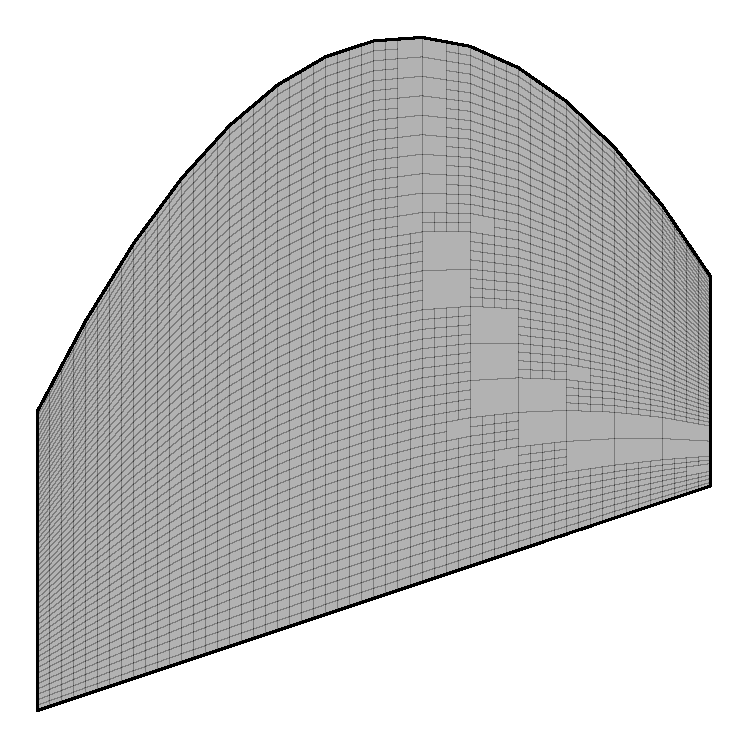
\includegraphics[width=0.43\textwidth]{fig_multiple_16a}}
\qquad
\subfigure[\label{fig_multiple_16b}]{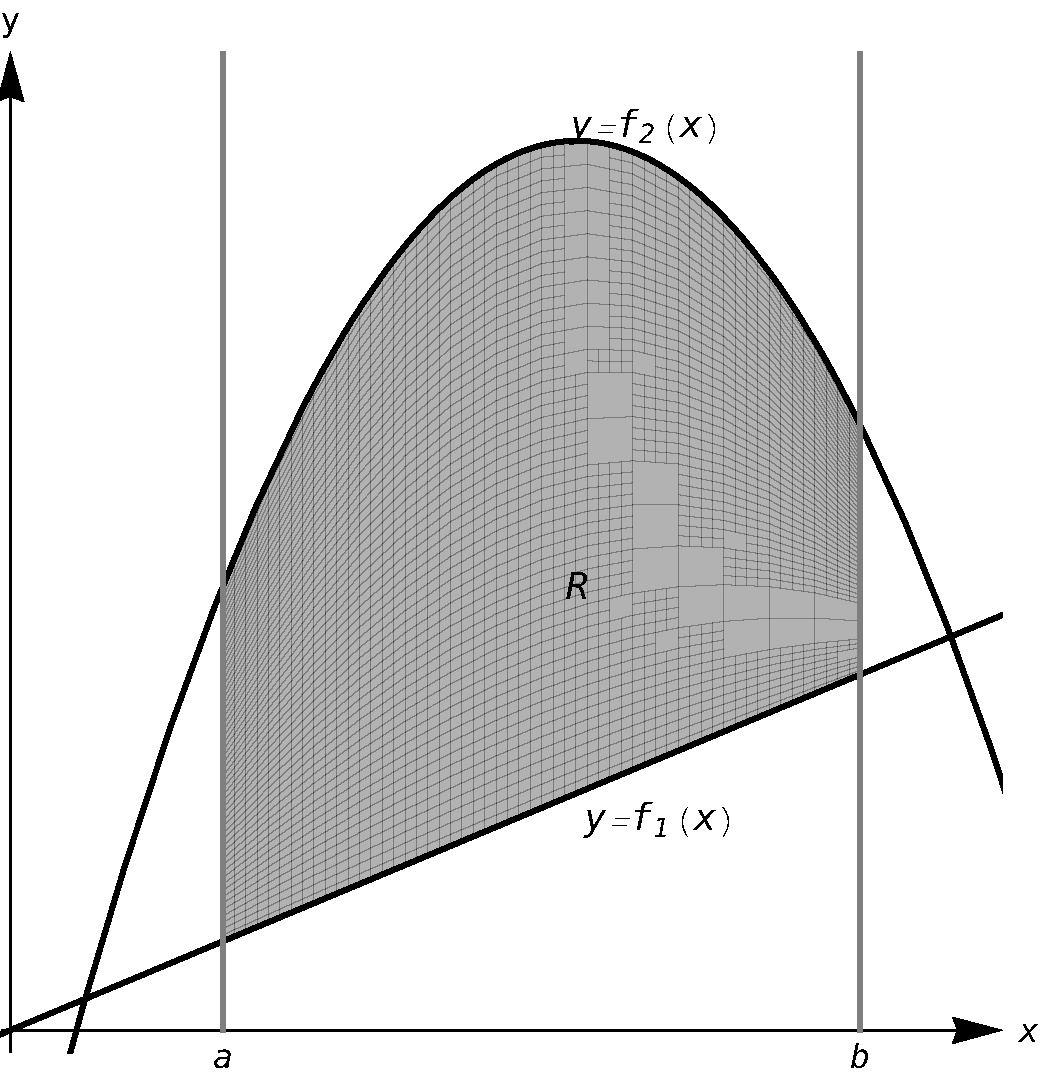
\includegraphics[width=0.43\textwidth]{fig_multiple_16b} }
\caption{Illustrating the concept of a lamina.}
\end{figure}


We can write a simple double integral that represents the mass of the lamina: $\iint_R\ dm$, where $dm$ means a little mass. That is, the double integral states the total mass of the lamina can be found by summing up lots of little masses over $R$. To evaluate this double integral, partition $R$ into $n$ subregions as we have done in the past. The $i^{\,\text{th}}$ subregion has area $\Delta A_i$. 
A fundamental property of mass is that ``mass=density$\times$area''. If the lamina has a constant density $\delta$, then the mass of this $i^{\,\text{th}}$ subregion is $\Delta m_i=\delta\Delta A_i$. %then $dm=\delta\ dA$. 
That is, we can compute a small amount of mass by multiplying a small amount of area by the density.

If density is variable, with density function $\delta= \delta(x,y)$, then we can approximate the mass of the $i^{\,\text{th}}$ subregion of $R$ by multiplying $\Delta A_i$ by $\delta(x_i,y_i)$, where $(x_i,y_i)$ is a point in that subregion. That is, for a small enough subregion of $R$, the density across that region is almost constant. 

Note that mass and weight are different measures. Since they are scalar multiples of each other, it is often easy to treat them as the same measure. Here,  we effectively treat them as the same, as our technique for finding mass is the same as for finding weight. The density functions used will simply have different units.

The total mass $M$ of the lamina is approximately the sum of approximate masses of subregions:
$$M \approx \sum_{i=1}^n \Delta m_i = \sum_{i=1}^n \delta(x_i,y_i)\Delta A_i.$$

Taking the limit as the size of the subregions shrinks to 0 gives us the actual mass; that is, integrating $\delta(x,y)$ over $R$ gives the mass of the lamina:
\begin{equation}
M = \iint_R\ dm = \iint_R \delta(x,y)\ dA.
\label{def:mass}
\end{equation}

\begin{example}\label{ex_mass2}
Find the mass of a square lamina, represented by the unit square with lower lefthand corner at the origin, with variable density $\delta(x,y) = (x+y+2)$g/cm$^2$.

\xhrulefill{gray}{2.5pt}Solution \xhrulefill{gray}{2.5pt}

The variable density $\delta$, in this example, is very uniform, giving a density of 3 in the centre of the square and changing linearly. A graph of $\delta(x,y)$ can be seen in Figure \ref{fig_multiple_17}; notice how same amount of density is above $z=3$ as below. We'll comment on the significance of this momentarily.

The mass $M$ is found by integrating $\delta(x,y)$ over $R$. The order of integration is not important; we choose $dx\ dy$ arbitrarily. Thus:
\allowdisplaybreaks
\begin{align*}
M = \iint_R(x+y+2)\ dA &= \int\limits_0^1\int\limits_0^1 (x+y+2)\ dx\ dy\\
		&= \int\limits_0^1\left.\left(\frac 12x^2+x(y+2)\right)\right|_0^1dy\\
		&= \int\limits_0^1 \left(\frac52+y\right)\ dy\\
		&= \left.\left(\frac52y+\frac12y^2\right)\right|_0^1= 3\text{g}.
\end{align*}
It turns out that since the density of the lamina is so uniformly distributed above and below $z=3$ that the mass of the lamina is the same as if it had a constant density of 3. The density function $\delta=3$g/cm$^2$ and the one from this example are graphed in Figure \ref{fig_multiple_17}, which illustrates this concept.

\begin{figure}[H]
	\begin{center}
			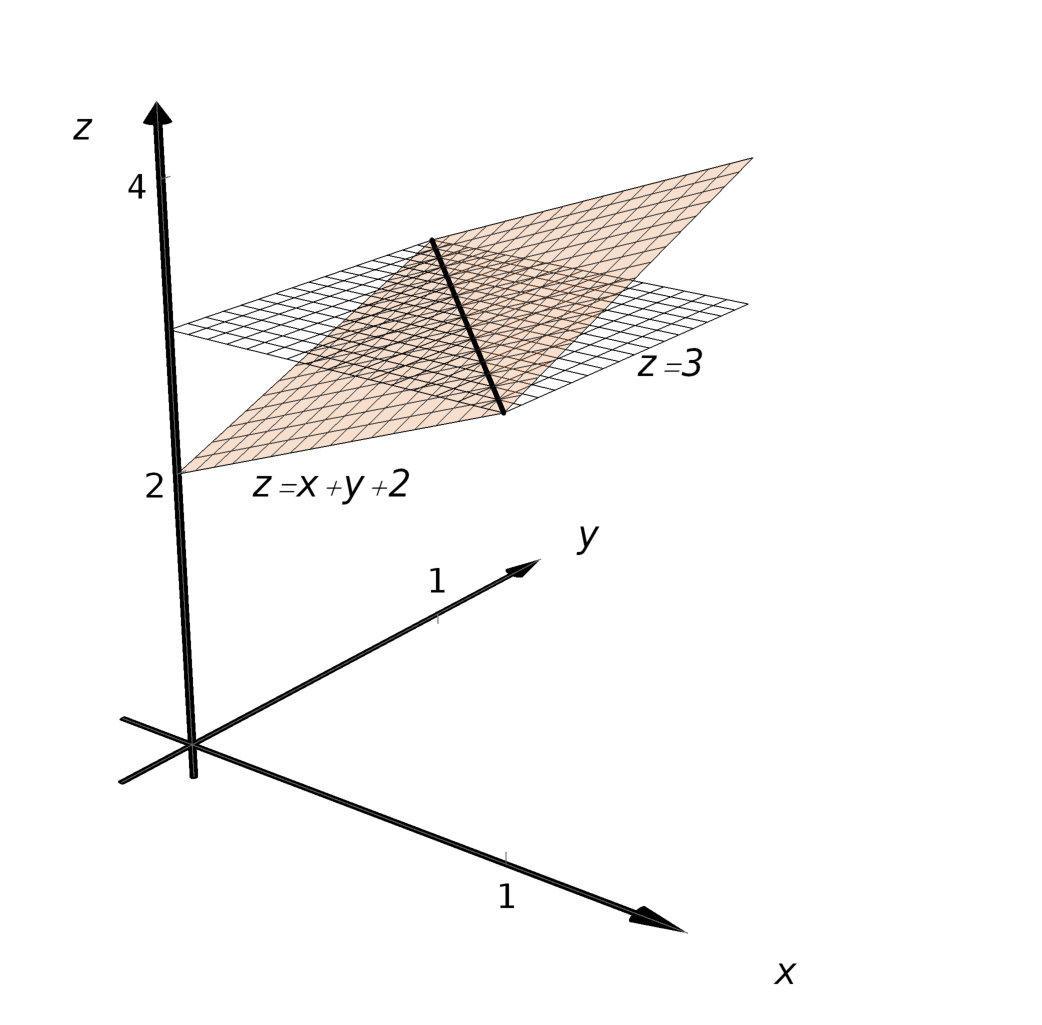
\includegraphics[width=0.5\textwidth]{fig_multiple_17}
	\caption{Graphing the density functions $\delta=3$g/cm$^2$ and $\delta(x,y) = (x+y+2)$g/cm$^2$.}
	\label{fig_multiple_17}
	\end{center}
\end{figure}


\end{example}

\begin{example}\label{ex_mass3}
Find the weight of the lamina represented by the disk with radius 2cm, centred at the origin, with density function $\delta(x,y) = (x^2+y^2+1)$g/cm$^2$. Compare this to the weight of the lamina with the same shape and density $\delta(x,y) = (2\sqrt{x^2+y^2}+1)$g/cm$^2$.

\xhrulefill{gray}{2.5pt}Solution \xhrulefill{gray}{2.5pt}

A direct application of Equation~\eqref{def:mass} states that the weight of the lamina is $\iint_R\delta(x,y)\ dA$. Since our lamina is in the shape of a circle, it makes sense to approach the double integral using polar coordinates.

The density function $\delta(x,y) = x^2+y^2+1$ becomes $$\delta(r,\theta) = (r\cos(\theta))^2+(r\sin(\theta))^2+1 = r^2+1.$$ The circle is bounded by $0\leq r\leq 2$ and $0\leq\theta\leq2\pi$. Thus the weight $W$ is:
\allowdisplaybreaks
\begin{align*}
W &= \int\limits_0^{2\pi}\int\limits_0^2 (r^2+1)r\ dr\ d\theta\\
	&= \int\limits_0^{2\pi} \left.\left(\frac14r^4+\frac12r^2\right)\right|_0^2d\theta\\
	&= \int\limits_0^{2\pi} 6 \ d\theta\\
	&= 12\pi \approx 37.70\text{g}.
\end{align*}

Now compare this with the density function $\delta(x,y) = 2\sqrt{x^2+y^2}+1$. Converting this to polar coordinates gives $$\delta(r,\theta) = 2\sqrt{\Big(r\cos(\theta)\Big)^2+\Big(r\sin(\theta)\Big)^2}+1 = 2r+1.$$ Thus the weight $W$ is:
\begin{align*}
W &= \int\limits_0^{2\pi}\int\limits_0^2 (2r+1)r\ dr\ d\theta\\
	&= \int\limits_0^{2\pi} \left(\frac23r^3+\frac12r^2\right)\Big|_0^2d\theta\\
	&= \int\limits_0^{2\pi} \left(\frac{22}3\right)\ d\theta\\
	&= \frac{44}3\pi \approx 46.08\text{g}.
\end{align*}
One would expect different density functions to return different weights, as we have here. The density functions were chosen, though, to be similar: each gives a density of 1 at the origin and a density of 5 at the outside edge of the circle, as seen in Figure \ref{fig_multiple_18}.


Notice how $x^2+y^2+1 \leq 2\sqrt{x^2+y^2}+1$ over the circle; this results in less weight.
\end{example}

\begin{figure}
\centering
%\raisebox{0.5cm}{
\subfigure[\label{fig_multiple_18a}]{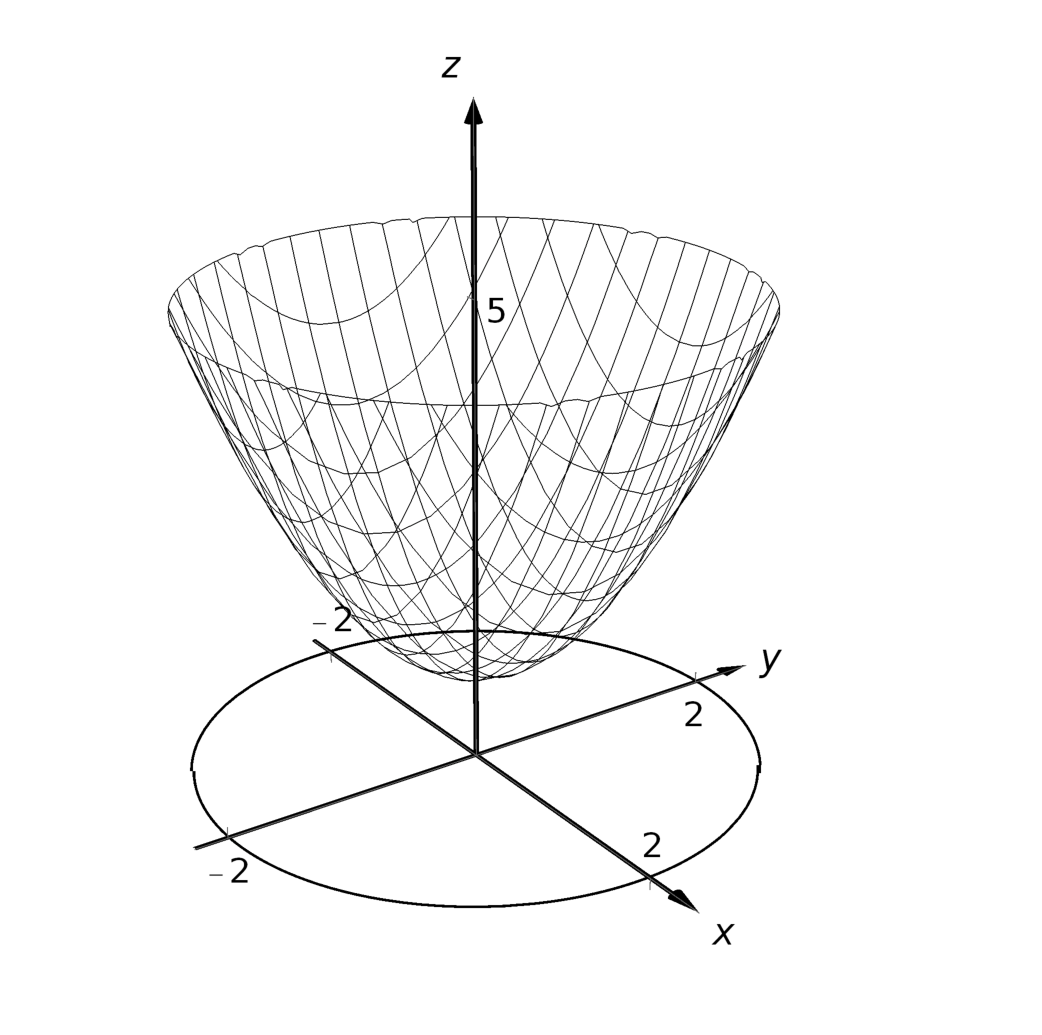
\includegraphics[width=0.43\textwidth]{fig_multiple_18a}}
\qquad
\subfigure[\label{fig_multiple_18b}]{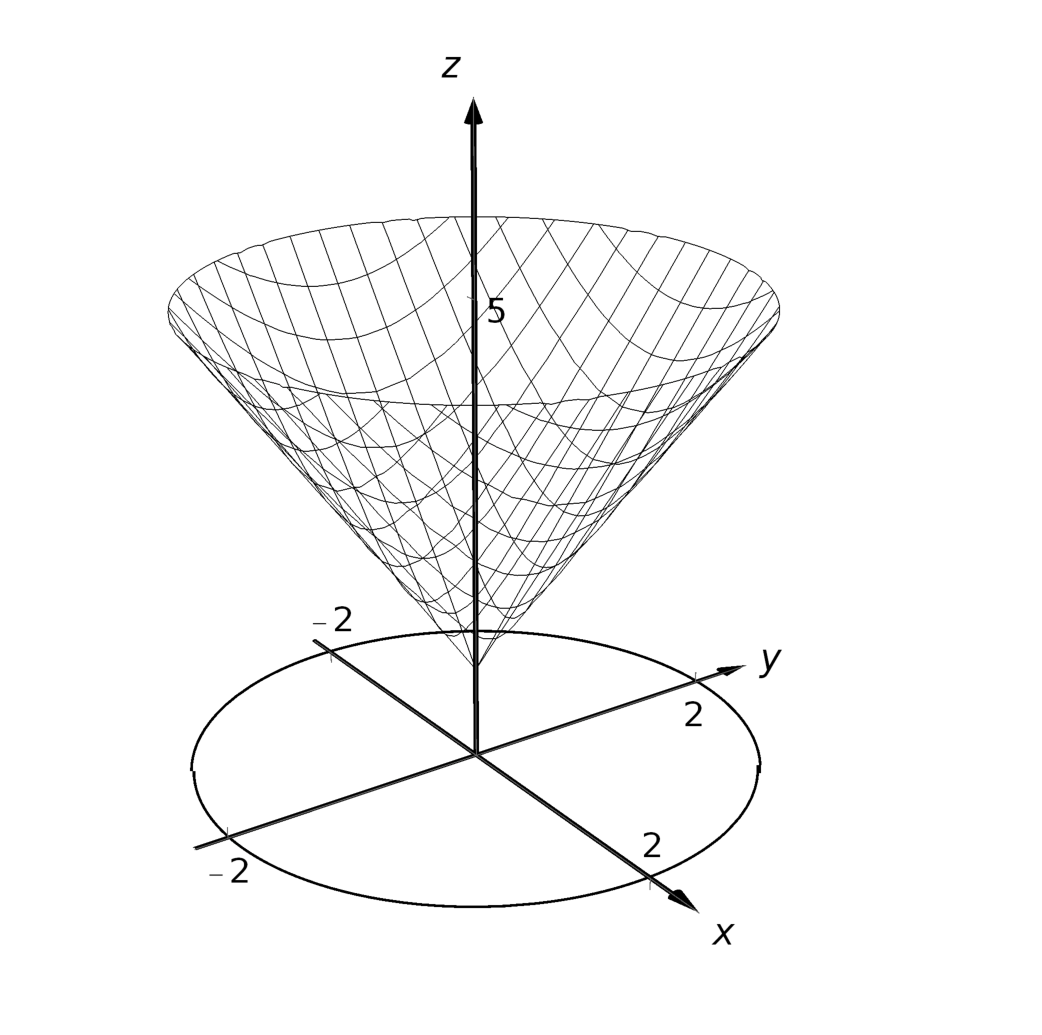
\includegraphics[width=0.43\textwidth]{fig_multiple_18b} }
\caption{Graphing the density functions  $\delta(x,y) = x^2+y^2+1$ (a) and $\delta(x,y) = 2\sqrt{x^2+y^2}+1$ (b).}
\label{fig_multiple_18}
\end{figure}

Plotting the density functions can be useful as our understanding of mass can be related to our understanding of volume under a surface. We interpreted $\iint_R f(x,y)\ dA$ as giving the volume under $f$ over $R$; we can understand $\iint_R\delta(x,y)\ dA$ in the same way. The volume under $\delta$ over $R$ is actually mass; by compressing the volume under $\delta$ onto the $xy$-plane, we get more mass in some areas than others -- i.e., areas of greater density.

Knowing the mass of a lamina is one of several important measures. Another is the centre of mass, which we discuss next.

\subsection{Centre of mass}

Consider a disk of radius 1 with uniform density. It is common knowledge that the disk will balance on a point if the point is placed at the centre of the disk. What if the disk does not have a uniform density? Through trial-and-error, we should still be able to find a spot on the disk at which the disk will balance on a point. This balance point is referred to as the \textbf{centre of mass} (\textit{massamiddelpunt}), or \textbf{centre of gravity} (\textit{zwaartepunt}). It is though all the mass is centred there. In fact, if the disk has a mass of 3kg, the disk will behave physically as though it were a point mass of 3kg located at its centre of mass. For instance, the disk will naturally spin with an axis through its centre of mass.
\index{centre of mass}\index[aut]{massamiddelpunt}

We find the centre of mass based on the principle of a weighted average. Consider a college class in which your homework average is 90\%, your test average is 73\%, and your final exam grade is an 85\%. Experience tells us that our final grade is not the \textit{average} of these three grades: that is, it is not:
$$\frac{0.9+0.73+0.85}{3} \approx 0.837 = 83.7\text{\%}.$$
That is, you are probably not pulling a B in the course. Rather, your grades are weighted. Let us say the homework is worth 10\% of the grade, tests are 60\% and the exam is 30\%. Then your final grade is:
$$(0.1)(0.9) + (0.6)(0.73)+(0.3)(0.85) = 0.783 = 78.3\text{\%}.$$
Each grade is multiplied by a weight. 

In general, given values $x_1,x_2,\ldots,x_n$ and weights $w_1,w_2,\ldots,w_n$, the weighted average of the $n$-values is
$$\dfrac{\ds\sum_{i=1}^n w_ix_i}{\ds\sum_{i=1}^n w_i}.$$

How this relates to centre of mass is given in the following definition.

\begin{definition}[Centre of mass of a discrete linear system]\label{thm:center_mass_points}
Let point masses $m_1,m_2,\ldots,m_n$ be distributed along the $x$-axis at locations $x_1,x_2,\ldots,x_n$, respectively. The \textbf{centre of mass $\overline{x}$} of the system is located at
\index{centre of mass}\index[aut]{massamiddelpunt}
$$\overline{x} = \dfrac{\ds\sum_{i=1}^nm_ix_i}{\ds\sum_{i=1}^n m_i}.$$
\end{definition}

In a discrete system (i.e., mass is located at individual points, not along a continuum) we find the centre of mass by dividing the mass into a \textbf{moment} (\textit{moment}) of the system. In general, a moment is a weighted measure of distance from a particular point or line. In the case described by Definition \ref{thm:center_mass_points}, we are finding a weighted measure of distances from the $y$-axis, so we refer to this as \textbf{the moment about the $y$-axis} (\textit{moment om de $y$-as}), represented by $M_y$.  Letting $M$ be the total mass of the system, we have  $\overline{x} = M_y/M$. 

We can extend the concept of the centre of mass of discrete points along a line to the centre of mass of discrete points in the plane rather easily. To do so, we define some terms then give a theorem.


\begin{definition}[Moments about the $x$- and $y$- axes]\label{def:moment}
Let point masses $m_1$, $m_2,\ldots,m_n$ be located at points $(x_1,y_1)$, $(x_2,y_2)\ldots,(x_n,y_n)$, respectively, in the $xy$-plane. \index{moment}\index[aut]{moment}
\begin{enumerate}[align=left]
	\item The \textbf{moment about the $x$-axis}, $M_x$, is 
	$$\ds M_x = \sum_{i=1}^n m_iy_i.$$
	\item The \textbf{moment about the $y$-axis}, $M_y$, is 
	$$\ds M_y = \sum_{i=1}^n m_ix_i.$$
	\end{enumerate}
\end{definition}

We now define the centre of mass of discrete points in the plane.

\begin{definition}[Centre of mass of a discrete planar system]\label{thm:center_mass_points_plane}
Let point masses $m_1$, $m_2,\ldots,m_n$ be located at points $(x_1,y_1)$, $(x_2,y_2)\ldots,(x_n,y_n)$, respectively, in the $xy$-plane, and let $\ds M = \sum_{i=1}^n m_i$.  
\index{centre of mass}\index[aut]{massamiddelpunt}

The \textbf{centre of mass} of the system is at $(\overline{x},\overline{y})$, where 
$$\overline{x}= \frac{M_y}{M}\quad \text{and}\quad \overline{y} = \frac{M_x}{M}.$$

\end{definition}

\begin{example}\label{ex_mass5}
Let point masses of 1kg, 2kg and 5kg be located at points $(2,0)$, $(1,1)$ and $(3,1)$, respectively, and are connected by thin rods of negligible weight. Find the centre of mass of the system.

\xhrulefill{gray}{2.5pt}Solution \xhrulefill{gray}{2.5pt}


We follow Definitions~\ref{thm:center_mass_points_plane} and \ref{def:moment} to find $M$, $M_x$ and $M_y$:

$M = 1+2+5 = 8$kg.

\noindent\begin{minipage}{.5\linewidth}
\begin{align*}
M_x &=  \sum_{i=1}^n m_iy_i \\
		&= 1(0) + 2(1) + 5(1) \\
		&= 7.
\end{align*}
\end{minipage}
\begin{minipage}{.5\linewidth}
\begin{align*}
M_y &=  \sum_{i=1}^n m_ix_i \\
		&= 1(2) + 2(1) + 5(3) \\
		&= 19.
\end{align*}
\end{minipage}

Thus the centre of mass is $$\ds (\overline{x},\overline{y}) = \left(\frac{M_y}{M},\frac{M_x}M\right) = \left(\frac{{19}}8,\frac78\right)  =(2.375,0.875),$$ illustrated in Figure \ref{fig_multiple_19}.

\begin{figure}[H]
	\begin{center}
			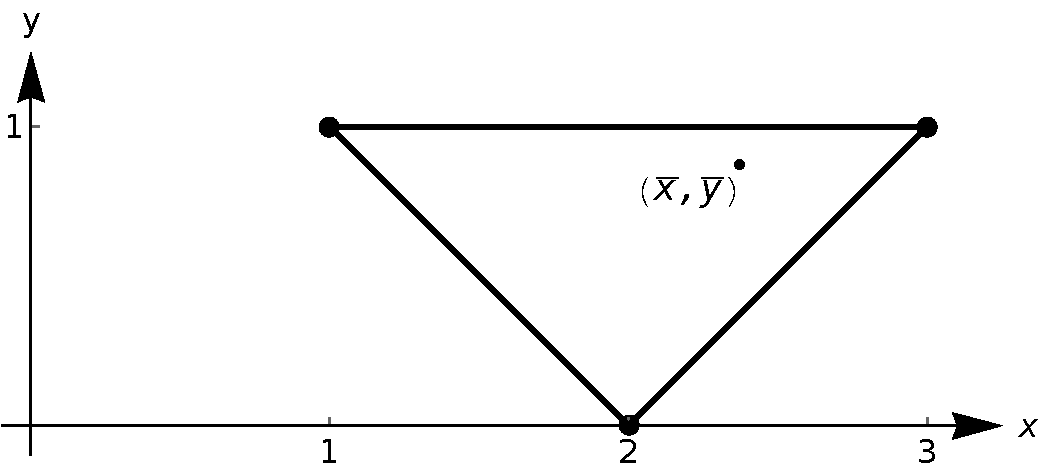
\includegraphics[width=0.5\textwidth]{fig_multiple_19}
	\caption{Illustrating the centre of mass of a discrete planar system in Example \ref{ex_mass5}.}
	\label{fig_multiple_19}
	\end{center}
\end{figure}

\end{example}

We finally arrive at our true goal of this section: finding the centre of mass of a lamina with variable density. While the above measurement of centre of mass is interesting, it does not directly answer more realistic situations where we need to find the centre of mass of a contiguous region. However, understanding the discrete case allows us to approximate the centre of mass of a planar lamina; using calculus, we can refine the approximation to an exact value.

We begin by representing a planar lamina with a region $R$ in the $xy$-plane with density function $\delta(x,y)$. Partition $R$ into $n$ subdivisions, each with area $\Delta A_i$. As done before, we can approximate the mass of the $i^{\,\text{th}}$ subregion with $\delta(x_i,y_i)\Delta A_i$, where $(x_i,y_i)$ is a point inside the $i^{\,\text{th}}$ subregion. We can approximate the moment of this subregion about the $y$-axis with $x_i\delta(x_i,y_i)\Delta A_i$ -- that is, by multiplying the approximate mass of the region by its approximate distance from the $y$-axis. Similarly, we can approximate the moment about the $x$-axis with $y_i\delta(x_i,y_i)\Delta A_i$. By summing over all subregions, we have:
\begin{align*}
\text{mass: } M &\approx \sum_{i=1}^n \delta(x_i,y_i)\Delta A_i\,, \qquad \text{(as seen before)}\\
\text{moment about the $x$-axis: } M_x &\approx \sum_{i=1}^n y_i\delta(x_i,y_i)\Delta A_i\,,\\
\text{moment about the $y$-axis: } M_y &\approx \sum_{i=1}^n x_i\delta(x_i,y_i)\Delta A_i\,.\\
\end{align*}

By taking limits, where size of each subregion shrinks to 0 in both the $x$- and $y$- directions, we arrive at the double integrals given in the following definition.

\begin{definition}[Centre of mass of a planar lamina]\label{thm:center_of_mass}
Let a planar lamina be represented by a closed, bounded region $R$ in the $xy$-plane with density function $\delta(x,y)$. Then we can infer the following information about the lamina: \index{centre of mass}\index{moment}\index[aut]{massamiddelpunt}\index[aut]{moment}
\begin{enumerate}
	\item The \textbf{mass} (\textit{massa}) of a planar lamina is $\ds M = \iint_R\delta(x,y)\ dA$.
	\item The \textbf{moment about the $x$-axis} is $\ds  M_x = \iint_Ry\delta(x,y)\ dA$.
	\item The \textbf{moment about the $y$-axis} is $\ds  M_y = \iint_Rx\delta(x,y)\ dA$.
	\item The \textbf{centre of mass} (\textit{massamiddelpunt}) of the object is
	$$(\overline{x},\overline{y}) = \left(\frac{M_y}{M},\frac{M_x}M\right).$$
\end{enumerate}
\end{definition}

We  practice  finding centres of mass by revisiting some of the lamina used previously in this section when finding mass. We will  just set up the integrals needed to compute $M$, $M_x$ and $M_y$ and leave the details of the integration to the reader.

\begin{example}
Find the centre of mass of a square lamina, represented by the unit square with lower lefthand corner at the origin (see Figure \ref{fig_multiple_17}), with variable density $\delta(x,y) = (x+y+2)$g/cm$^2$. This is the lamina from Example \ref{ex_mass2}.

\xhrulefill{gray}{2.5pt}Solution \xhrulefill{gray}{2.5pt}

We follow Theorem \ref{thm:center_of_mass}, to find $M$, $M_x$ and $M_y$:
\begin{align*}
M &= \iint_R (x+y+2)\ dA = \int\limits_0^1\int\limits_0^1 (x+y+2)\ dx\ dy =3\text{g}.\\
M_x &= \iint_R y(x+y+2)\ dA = \int\limits_0^1\int\limits_0^1 y(x+y+2)\ dx\ dy =\frac{19}{12}.\\
M_y &= \iint_R x(x+y+2)\ dA = \int\limits_0^1\int\limits_0^1 x(x+y+2)\ dx\ dy =\frac{19}{12}.
\end{align*}
Thus the centre of mass is $$\ds (\overline{x},\overline{y}) = \left(\frac{M_y}M,\frac{M_x}M\right) = \left(\frac{19}{36},\frac{19}{36}\right) \approx (0.528,0.528).$$ While the mass of this lamina is the same as the lamina in the previous example, the greater density found with greater $x$- and $y$-values pulls the centre of mass from the centre slightly towards the upper righthand corner.
\end{example}

\begin{example}\label{ex_mass8}
Find the centre of mass of the lamina represented by the circle with radius 2cm, centred at the origin, with density function $\delta(x,y) = (x^2+y^2+1)$g/cm$^2$. This is one of the lamina used in Example \ref{ex_mass3}.

\xhrulefill{gray}{2.5pt}Solution \xhrulefill{gray}{2.5pt}

As done in Example \ref{ex_mass3}, it is best to describe $R$ using polar coordinates.
Thus when we compute $M_y$, we will integrate not $x\delta(x,y) = x(x^2+y^2+1)$, but rather $\big(r\cos(\theta)\big)\delta(r\cos(\theta),r\sin(\theta))$\linebreak $= \big(r\cos(\theta)\big)\big(r^2+1\big).$ We compute $M$, $M_x$ and $M_y$:
\allowdisplaybreaks
\begin{align*}
M &= \int\limits_0^{2\pi}\int\limits_0^2 (r^2+1)r\ dr\ d\theta = 12\pi\approx 37.7\text{g}\,,\\
M_x &= \int\limits_0^{2\pi}\int\limits_0^2 (r\sin(\theta))(r^2+1)r \ dr\ d\theta = 0\,,\\
M_y &= \int\limits_0^{2\pi}\int\limits_0^2 (r\cos(\theta))(r^2+1)r \ dr\ d\theta = 0\,.\\
\end{align*}
Since $R$ and the density of $R$ are both symmetric about the $x$- and $y$-axes, it should come as no big surprise that the moments about each axis is 0. Thus the centre of mass is $(\overline{x},\overline{y})=(0,0)$. 
\end{example}

\section{Surface area}\label{sec:surface_area}
	\checkoddpage
\marginpar{\ifoddpage\hspace*{-1.5cm}\else\hspace*{0.25cm}\fi
\includegraphics[width=0.075\textwidth]{youtube}\\
\ifoddpage\hspace*{-1.75cm}\else\hspace*{0.1cm}\fi
\qrcode[height=1.75cm]{https://youtu.be/GSDrQYq_Iww}
%\includegraphics[width=0.1\textwidth]{surface_area_double}
}
In Section \ref{sec:arc_length} we used definite integrals to compute the arc length of plane curves of the form \linebreak $y=f(x)$. We later extended these ideas to compute the arc length of plane curves defined by parametric or polar equations. 

The natural extension of the concept of arc length over an interval to surfaces is surface area over a region. For that purpose, consider the surface $z=f(x,y)$ over a region $R$ in the $xy$-plane, shown in Figure \ref{fig_multiple_20a}. Because of the domed shape of the surface, the surface area will be greater than that of the area of the region $R$. We can find this area using the same basic technique we have used over and over: we'll make an approximation, then using limits, we'll refine the approximation to the exact value.


\begin{figure}
\centering
%\raisebox{0.5cm}{
\subfigure[\label{fig_multiple_20a}]{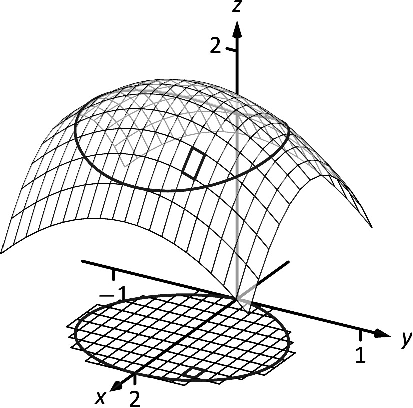
\includegraphics[width=0.43\textwidth]{fig_multiple_20a}}
\qquad
\subfigure[\label{fig_multiple_20b}]{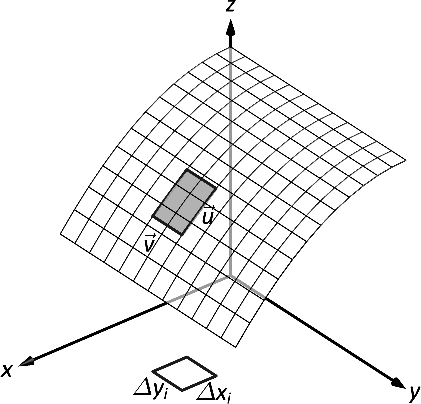
\includegraphics[width=0.43\textwidth]{fig_multiple_20b} }
\caption{Developing a method of computing surface area.}
\end{figure}



As done to find the volume under a surface or the mass of a lamina, we subdivide $R$ into $n$ subregions. Here we subdivide $R$ into rectangles, as shown in the figure. One such subregion is outlined in the figure, where the rectangle has dimensions $\dx_i$ and $\dy_i$, along with its corresponding region on the surface.

In Figure~\ref{fig_multiple_20b}, we zoom in on this portion of the surface. When $\dx_i$ and $\dy_i$ are small, the function is approximated well by the tangent plane at any point $(x_i,y_i)$ in this subregion, which is graphed in part (b). In fact, the tangent plane approximates the function so well that in this figure, it is virtually indistinguishable from the surface itself! Therefore we can approximate the surface area $S_i$ of this region of the surface with the area $T_i$ of the corresponding portion of the tangent plane.

This portion of the tangent plane is a parallelogram, defined by sides $\vec u$ and $\vec v$, as shown. One of the applications of the cross product from Section \ref{sec:cross_product} is that the area of this parallelogram is $\norm{\vec u\times \vec v}$. So, once we can determine $\vec u$ and $\vec v$, we can determine the area.

$\vec u$ is tangent to the surface in the direction of $x$, therefore, from Section \ref{sec:multi_tangent}, $\vec u$ is parallel to $\left( 1,0,f_x(x_i,y_i)\right)$. The $x$-displacement of $\vec u$ is $\dx_i$, so we know that $\vec u = \dx_i\left( 1,0,f_x(x_i,y_i)\right)$. Similar logic shows that $\vec v = \dy_i\left( 0,1,f_y(x_i,y_i)\right)$.Thus:
\begin{align*}
\text{surface area $S_i$} &\approx \text{area of  $T_i$}\\
				&= \norm{\vec u\times \vec v}\\[0.2cm]
				&= \big|\big|\dx_i\left( 1,0,f_x(x_i,y_i)\right)\times\dy_i\left( 0,1,f_y(x_i,y_i)\right)\big|\big|\\[0.2cm]
				&=\sqrt{1+f_x(x_i,y_i)^2+f_y(x_i,y_i)^2}\dx_i\dy_i.
\end{align*}
Note that $\dx_i\dy_i = \Delta A_i$, the area of the $i^{\,\text{th}}$ subregion.

Summing up all $n$ of the approximations to the surface area gives
$$\text{surface area over $R$} \approx \sum_{i=1}^n \sqrt{1+f_x(x_i,y_i)^2+f_y(x_i,y_i)^2}\Delta A_i.$$

Once again take a limit as all of the $\dx_i$ and $\dy_i$ shrink to 0; this leads to a double integral:
\begin{equation}
SA=\iint_R \sqrt{1+f_x(x,y)^2+f_y(x,y)^2}\ dA.
\label{def:surfacearea}
\end{equation}

We use this definition to compute surface areas of known surfaces. 

\begin{example}\label{ex_surfacearea2}
Find the surface area of the sphere with radius $a$ centred at the origin, whose top hemisphere has equation $f(x,y)=\sqrt{a^2-x^2-y^2}$. 

\xhrulefill{gray}{2.5pt}Solution \xhrulefill{gray}{2.5pt}

We start by computing partial derivatives and find 
$$f_x(x,y) = \frac{-x}{\sqrt{a^2-x^2-y^2}} \quad \text{and}\quad f_y(x,y) = \frac{-y}{\sqrt{a^2-x^2-y^2}}.$$
As our function $f$ only defines the top upper hemisphere of the sphere, we double our surface area result to get the total area:
\begin{align*}
SA & = 2\iint_R \sqrt{1+ f_x(x,y)^2+f_y(x,y)^2}\ dA \\
		&= 2\iint_R \sqrt{1+ \frac{x^2+y^2}{a^2-x^2-y^2}}\ dA.
\end{align*}
The region $R$ that we are integrating over is bounded by the circle, centered at the origin, with radius $a$: $x^2+y^2=a^2$. Because of this region, we are likely to have greater success with our integration by converting to polar coordinates. Using the substitutions $x=r\cos(\theta)$, $y=r\sin(\theta)$, $dA = r\ dr\ d\theta$ and bounds $0\leq\theta\leq2\pi$ and $0\leq r\leq a$, we have:
\begin{align}
SA &= 2\int\limits_0^{2\pi}\int\limits_0^a \sqrt{1+\frac{r^2\cos^2(\theta)+r^2\sin^2(\theta)}{a^2-r^2\cos^2(\theta)-r^2\sin^2(\theta)}}\ r\ dr\ d\theta \notag\\
&=2\int\limits_0^{2\pi}\int\limits_0^ar\sqrt{1+\frac{r^2}{a^2-r^2}}\ dr\ d\theta\notag\\
&=2\int\limits_0^{2\pi}\int\limits_0^ar\sqrt{\frac{a^2}{a^2-r^2}}\ dr\ d\theta.\label{eq:exsurfacearea2}
\intertext{Apply substitution $u=a^2-r^2$ and integrate the inner integral, giving}
&= 2\int\limits_0^{2\pi} a^2\ d\theta\notag\\
&= 4\pi a^2\notag.
\end{align}
Our work confirms the known formula.

Note that the inner integral in Equation \eqref{eq:exsurfacearea2} is an improper integral, as its is not defined at $r=a$. To properly evaluate this integral, one must use the techniques of Section \ref{sec:improper_integration}.  Since the resulting improper integral does converge, the surface area is accurately computed.
\end{example}

\begin{example}\label{ex_surfacearea4}
Find the area of the surface $f(x,y) = x^2-3y+3$ over the region $R$ bounded by $-x\leq y\leq x$, $0\leq x\leq 4$, as pictured in Figure \ref{fig_multiple_21}.

\begin{figure}[H]
	\begin{center}
			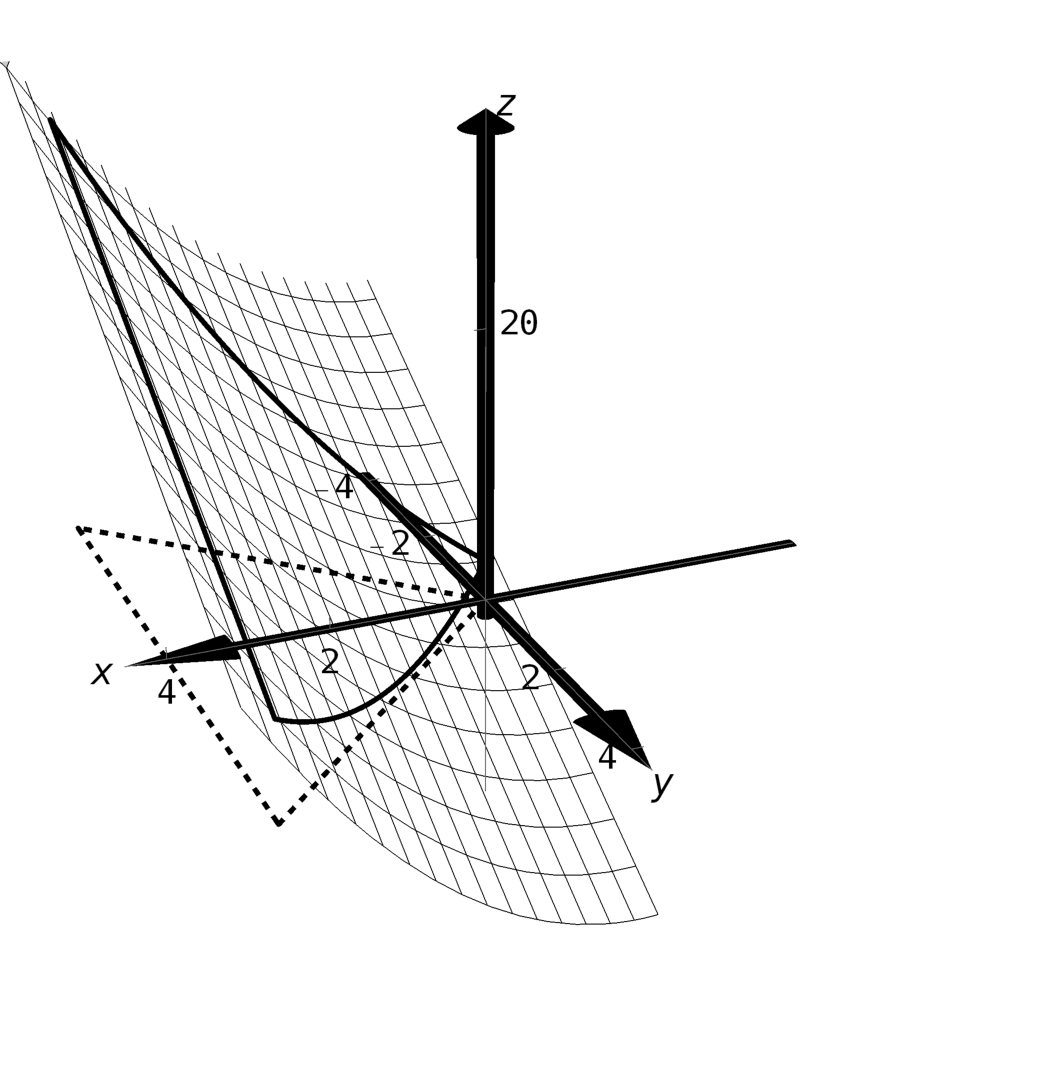
\includegraphics[width=0.5\textwidth]{fig_multiple_21}
	\caption{Graphing the surface in Example \ref{ex_surfacearea4}.}
	\label{fig_multiple_21}
	\end{center}
\end{figure}

\xhrulefill{gray}{2.5pt}Solution \xhrulefill{gray}{2.5pt}

It is straightforward to compute $f_x(x,y) = 2x$ and $f_y(x,y) = -3$. Thus the surface area is described by the double integral
$$\iint_R \sqrt{1+(2x)^2+(-3)^2}\ dA = \iint_R \sqrt{10+4x^2}\ dA.$$
As with integrals describing arc length, double integrals describing surface area are in general hard to evaluate directly because of the square root. This particular integral can be easily evaluated, though, with judicious choice of our order of integration. 

Integrating with order $dx\ dy$ requires us to evaluate $\int\limits \sqrt{10+4x^2}\ dx$. This can be done, though it involves the goniometric substitution $2x=\sqrt{10}\,\tan(t)$. Integrating with order $dy\ dx$ has as its first integral $\int\limits \sqrt{10+4x^2}\ dy$, which is easy to evaluate: it is simply $y\sqrt{10+4x^2}+C$. So we proceed with the order $dy\ dx$.
\allowdisplaybreaks
\begin{align*}
SA &= \iint_R\sqrt{10+4x^2}\ dA \\
            &= \int\limits_0^4\int\limits_{-x}^x\sqrt{10+4x^2}\ dy \ dx\\
				&= \int\limits_0^4\left.\left(y\sqrt{10+4x^2}\right)\right|_{-x}^x dx\\
				&=\int\limits_0^4 2x\sqrt{10+4x^2} \ dx
				\intertext{Apply substitution with $u = 10+4x^2$:}
			SA	&= \left.\left(\frac16\big(10+4x^2\big)^{3/2}\right)\right|_0^4 \\
				&= \frac13\big(37\sqrt{74}-5\sqrt{10}\big) \approx 100.825\text{ units}^2.
\end{align*}
So while the region $R$ over which we integrate has an area of 16 \text{units}$^2$, the surface has a much greater area as its $z$-values change dramatically over $R$.
\end{example}


In practice, technology helps greatly in the evaluation of such integrals. High powered computer algebra systems can compute integrals that are difficult, or at least time consuming, by hand, and can at least produce very accurate approximations with numerical methods. In general, just knowing how to set up the proper integrals brings one very close to being able to compute the needed value. Most of the work is actually done in just describing the region $R$ in terms of polar or rectangular coordinates. Once this is done, technology can usually provide a good answer.


\section{Triple integration}\label{sec:triple_int}

\subsection{Volume between surfaces}
We learned in Section \ref{sec:double_int_volume} how to compute the signed volume $V$ under a surface $z=f(x,y)$ over a region $R$. It follows that if $f(x,y)\geq g(x,y)$ on $R$, then the volume between $f(x,y)$ and $g(x,y)$ on $R$ is 
$$V = \iint_R f(x,y)\ dA - \iint_R g(x,y)\ dA = \iint_R \big(f(x,y)-g(x,y)\big)\ dA.$$


Consider, for instance, the volume of the space region bounded by the planes $z=3x+y-4$, \\ $z=8-3x-2y$, $x=0$ and $y=0$. In Figure \ref{fig_multiple_22a} the planes are drawn; in Figure~\ref{fig_multiple_22b}, only the defined region is given. The region $R$ over which we will integrate is bounded by $x=0$, $y=0$ and the line of intersection of the planes  $z=3x+y-4$ and $z=8-3x-2y$, which is $y=4-2x$. So, we find  the volume by evaluating the integral 
$$\ds \int\limits_0^2\int\limits_0^{4-2x} \big(8-3x-2y-(3x+y-4)\big)\ dy\ dx=16.$$



Note how we can rewrite the integrand as an integral, much as we did in Section \ref{sec:iterated_integrals}:
$$8-3x-2y-(3x+y-4) = \int\limits_{3x+y-4}^{8-3x-2y}\ dz.$$
Thus we can rewrite the double integral that finds volume as
$$\int\limits_0^2\int\limits_0^{4-2x} \big(8-3x-2y-(3x+y-4)\big)\ dy\ dx = \int\limits_0^2\int\limits_0^{4-2x}\left(\int\limits_{3x+y-4}^{8-3x-2y}\ dz\right)\ dy\ dx.$$
This no longer looks like a double integral, but more like a triple integral.


\begin{figure}[h]
\centering
%\raisebox{0.5cm}{
\subfigure[\label{fig_multiple_22a}]{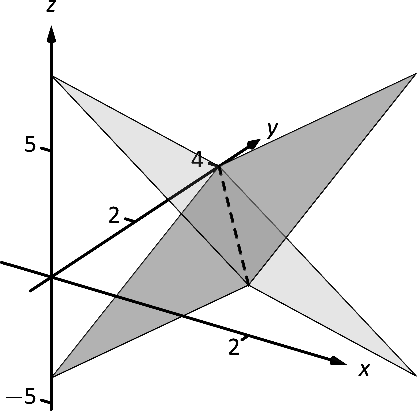
\includegraphics[width=0.37\textwidth]{fig_multiple_22a}}
\qquad
\subfigure[\label{fig_multiple_22b}]{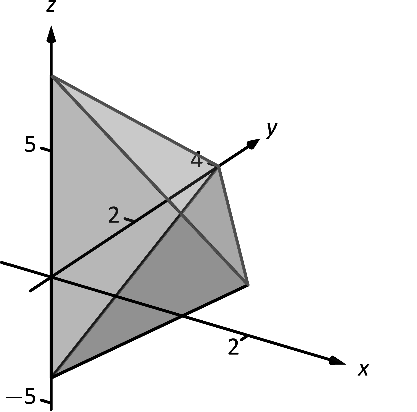
\includegraphics[width=0.37\textwidth]{fig_multiple_22b} }
\caption{Finding the volume between $z=3x+y-4$, $z=8-3x-2y$, $x=0$ and $y=0$.}
\end{figure}




To formally find the volume of a closed, bounded region $D$ in space, such as the one shown in Figure \ref{fig_multiple_23a}, we start with an approximation. Break $D$ into $n$ rectangular solids; the solids near the boundary of $D$ may possibly not include portions of $D$ and/or include extra space. In Figure \ref{fig_multiple_23b}, we zoom in on a portion of the boundary of $D$ to show a rectangular solid that contains space not in $D$; as this is an approximation of the volume, this is acceptable and this error will be reduced as we shrink the size of our solids.


\begin{figure}[h]
\centering
%\raisebox{0.5cm}{
\subfigure[\label{fig_multiple_23a}]{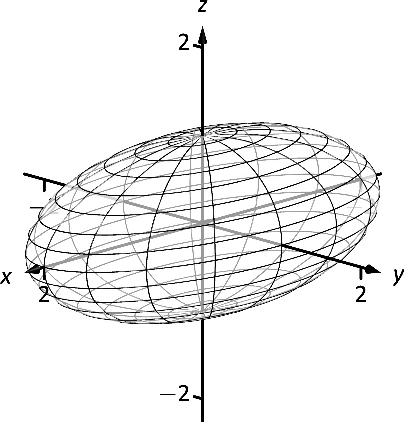
\includegraphics[width=0.4\textwidth]{fig_multiple_23a}}
\qquad
\subfigure[\label{fig_multiple_23b}]{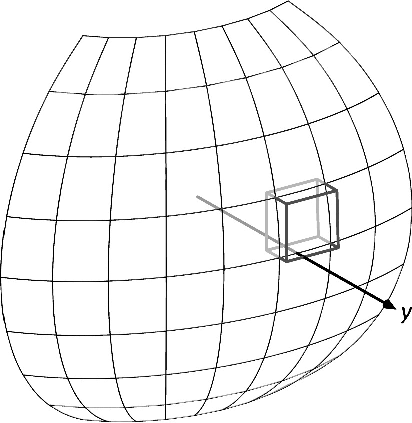
\includegraphics[width=0.4\textwidth]{fig_multiple_23b} }
\caption{Approximating the volume of a region $D$ in space.}
\end{figure}


The volume $\Delta V_i$ of the $i^\text{\,th}$ solid $D_i$ is $\Delta V_i = \dx_i\dy_i\ddz_i$, where $\dx_i$, $\dy_i$ and $\ddz_i$ give the dimensions of the rectangular solid in the $x$-, $y$- and $z$- directions, respectively. By summing up the volumes of all $n$ solids, we get an approximation of the volume $V$ of $D$:
$$V \approx \sum_{i=1}^n \Delta V_i = \sum_{i=1}^n \dx_i\dy_i\ddz_i.$$

Let $\mathcal{D}$ represent the length of the longest diagonal of rectangular solids in the subdivision of $D$. As $\mathcal{D}\to 0$, the volume of each solid goes to 0, as do each of $\dx_i$, $\dy_i$ and $\ddz_i$, for all $i$. Our calculus experience tells us that taking a limit as $\mathcal{D}\to 0$ turns our approximation of $V$ into an exact calculation of $V$. Before we state this result in a theorem, we use a definition to define some terms.




\begin{definition}[Triple integrals, iterated integration (Part I)]
\label{def:triple_integral}
Let $D$ be a closed, bounded region in space. Let $a$ and $b$ be real numbers, let $g_1(x)$ and $g_2(x)$ be continuous functions of $x$, and let $f_1(x,y)$ and $f_2(x,y)$ be continuous functions of $x$ and $y$.
\index{integration!triple}\index{triple integral}\index{iterated integration}
\begin{enumerate}
	\item	The volume $V$ of $D$ is denoted by a \textbf{triple integral} (\textit{drievoudige integraal})
	$$V = \iiint_D dV.$$
	
	\item The iterated integral 
	$$\ds \int\limits_a^b\int\limits_{g_1(x)}^{g_2(x)}\int\limits_{f_1(x,y)}^{f_2(x,y)} \ dz\ dy\ dx$$
	is evaluated as 
	$$\int\limits_a^b\int\limits_{g_1(x)}^{g_2(x)}\int\limits_{f_1(x,y)}^{f_2(x,y)} \ dz\ dy\ dx=\int\limits_a^b\int\limits_{g_1(x)}^{g_2(x)}\left(\int\limits_{f_1(x,y)}^{f_2(x,y)} \ dz\right)\ dy\ dx.$$

	
	
\end{enumerate}

\end{definition}

Our informal understanding of the notation $\iiint_D\ dV$ is sum up lots of little volumes over $D$, analogous to our understanding of $\iint_R\ dA$ and $\iint_R\ dm$.

We now state the major theorem of this section.

\begin{theorem}[Triple integration (Part I)]
\label{thm:triple_integration}
Let $D$ be a closed, bounded region in space and let $\Delta D$ be any subdivision of $D$ into $n$ rectangular solids, where the  $i^\text{\,th}$ subregion $D_i$ has dimensions $\dx_i\times\dy_i\times\ddz_i$ and volume $\Delta V_i$.
\index{integration!triple}\index{triple integral}\index{iterated integration}
\begin{enumerate}
	\item The volume $V$ of $D$ is
	$$V = \iiint_D\ dV = \lim_{\mathcal{D}\to0} \sum_{i=1}^n \Delta V_i = \lim_{\mathcal{D}\to0} \sum_{i=1}^n \dx_i\dy_i\ddz_i.$$
	
	\item		If $D$ is defined as the region bounded by the planes $x=a$ and $x=b$, the cylinders $y=g_1(x)$ and $y=g_2(x)$, and the surfaces $z=f_1(x,y)$ and $z=f_2(x,y)$, where $a<b$, $g_1(x)\leq g_2(x)$ and $f_1(x,y)\leq f_2(x,y)$ on $D$, then
	$$\iiint_D \ dV = \int\limits_a^b\int\limits_{g_1(x)}^{g_2(x)}\int\limits_{f_1(x,y)}^{f_2(x,y)} \ dz\ dy\ dx.$$
	
	\item		$V$ can be determined using iterated integration with other orders of integration (there are 6 total), as long as $D$ is defined by the region enclosed by a pair of planes, a pair of cylinders, and a pair of surfaces.
\end{enumerate}

\end{theorem}

	\checkoddpage
\marginpar{\ifoddpage\hspace*{-1.5cm}\else\hspace*{0.25cm}\fi
\includegraphics[width=0.075\textwidth]{youtube}\\
\ifoddpage\hspace*{-1.75cm}\else\hspace*{0.1cm}\fi
\qrcode[height=1.75cm]{https://youtu.be/mDrOpsyg16U}
%\includegraphics[width=0.1\textwidth]{order_int_triple}
}


We evaluated the area of a plane region $R$ by iterated integration, where the bounds were from curve to curve, then from point to point. Theorem \ref{thm:triple_integration} allows us to find the volume of a space region with an iterated integral with bounds from surface to surface, then from curve to curve, then from point to point. In the iterated integral 
$$\int\limits_a^b\int\limits_{g_1(x)}^{g_2(x)}\int\limits_{f_1(x,y)}^{f_2(x,y)} \ dz\ dy\ dx,$$
the bounds $a\leq x\leq b$ and $g_1(x)\leq y\leq g_2(x)$ define a region $R$ in the $xy$-plane over which the region $D$ exists in space. However, these bounds are also defining surfaces in space; $x=a$ is a plane and $y=g_1(x)$ is a cylinder. The combination of these six surfaces enclose, and define, $D$.

Examples will help us understand triple integration, including integrating with various orders of integration.


\begin{example}
\label{ex_trip2}
Find the volume of the space region in the first octant bounded by the plane $z=2-y/3-2x/3$, shown in Figure \ref{fig_multiple_24a}, using the order of integration $dz\ dy\ dx$. Set up the triple integrals that give the volume in the other five orders of integration.
\begin{figure}[H]
\centering
%\raisebox{0.5cm}{
\centerline{\subfigure[\label{fig_multiple_24a}]{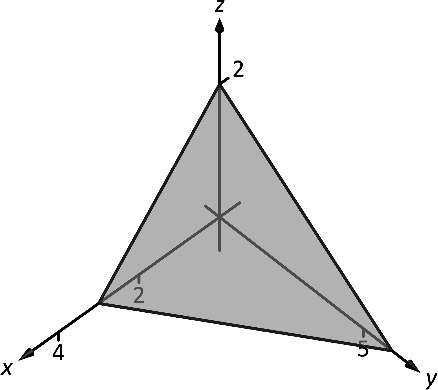
\includegraphics[width=0.43\textwidth]{fig_multiple_24a}}
\qquad
\subfigure[\label{fig_multiple_24b}]{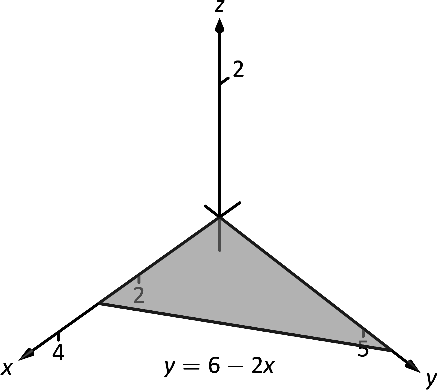
\includegraphics[width=0.43\textwidth]{fig_multiple_24b} }}

\centerline{\subfigure[\label{fig_multiple_24c}]{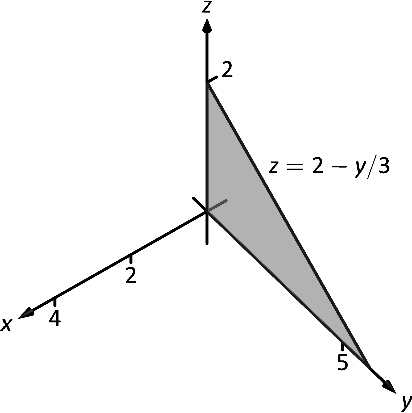
\includegraphics[width=0.43\textwidth]{fig_multiple_24c}}
\qquad
\subfigure[\label{fig_multiple_24d}]{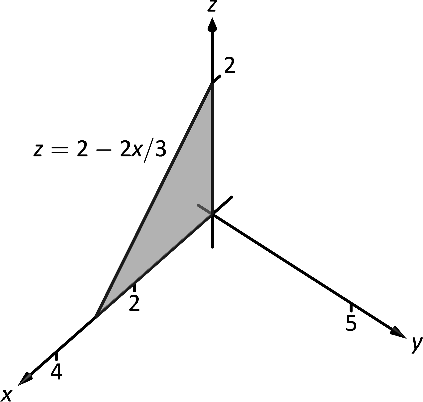
\includegraphics[width=0.43\textwidth]{fig_multiple_24d} }}
\caption{The region $D$ used in Example \ref{ex_trip2} in (a); the region found by projecting $D$ onto the $xy$- (b), $yz$- (c) and $xz$- (d) plane.}
\end{figure}

\xhrulefill{gray}{2.5pt}Solution \xhrulefill{gray}{2.5pt}

Starting with the order of integration $dz\ dy\ dx$, we need to first find bounds on $z$. The region $D$ is bounded below by the plane $z=0$ because we are restricted to the first octant and above by $z=2-y/3-2x/3$; $0\leq z\leq 2-y/3-2x/3$.

To find the bounds on $y$ and $x$, we project the region onto the $xy$-plane, giving the triangle shown in Figure \ref{fig_multiple_24b}.  We define that region $R$, in the integration order of $dy\ dx$, with bounds \\ $0\leq y\leq 6-2x$ and $0\leq x\leq 3$. Thus the volume $V$ of the region $D$ is:
\begin{align*}
V &= \iiint_D \ dV\\
		&= \int\limits_0^3\int\limits_0^{6-2x}\ \int\limits_0^{2-y/3-2x/3}\ dz\ dy\ dx %\\
		\end{align*}
		\begin{align*}
		&= \int\limits_0^3\int\limits_0^{6-2x}\left(\int\limits_0^{2-y/3-2x/3}\ dz\right)\ dy\ dx \\
		&=\int\limits_0^3\int\limits_0^{6-2x}(z)\Big|_0^{2-y/3-2x/3}\ dy\ dx \\
		&= \int\limits_0^3\int\limits_0^{6-2x}\left(2-\frac 13y-\frac 23x\right)\ dy\ dx.
		\intertext{From this step on, we are evaluating a double integral as done many times before. We skip these steps and give the final volume}
		V &= 6\text{ units}^3.		
\end{align*}

\noindent The order $dz\ dx\ dy$:\\[0.2cm]
Now consider the volume using the order of integration $dz\ dx\ dy$. The bounds on $z$ are the same as before, $0\leq z\leq 2-y/3-2x/3$. Projecting the space region on the $xy$-plane as shown in Figure \ref{fig_multiple_24b}, we now describe this triangle with the order of integration $dx\ dy$. This gives bounds $0\leq x\leq 3-y/2$ and $0\leq y\leq 6$. Thus the volume is given by the triple integral
$$V = \int\limits_0^6\int\limits_0^{3-y/2}\ \int\limits_0^{2-y/3-2x/3}\ dz\ dx\ dy.$$

\noindent The order $dx\ dy\ dz$:\\[0.2cm]
Following our surface to surface strategy, we need to determine the $x$-surfaces that bound our space region. To do so, approach the region from behind, in the direction of increasing $x$. The first surface we hit as we enter the region is the $yz$-plane, defined by $x=0$. We come out of the region at the plane $z=2-y/3-2x/3$; solving for $x$, we have $x= 3-y/2-3z/2$. Thus the bounds on $x$ are: $0\leq x\leq 3-y/2-3z/2$.

Now project the space region onto the $yz$-plane, as shown in Figure \ref{fig_multiple_24c}.  We need to find bounds on this region with the order $dy\ dz$. The curves that bound $y$ are $y=0$ and $y=6-3z$; the \textit{points} that bound $z$ are 0 and 2. Thus the triple integral giving volume is:
$$V =\int\limits_0^2\int\limits_0^{6-3z}\ \int\limits_0^{3-y/2-3z/2}\ dx\ dy\ dz.$$

\noindent The order $dx\ dz\ dy$:\\[0.2cm]
The $x$-bounds are the same as the order above. We now consider the triangle in Figure \ref{fig_multiple_24c} and describe it with the order $dz\ dy$: $0\leq z\leq 2-y/3$ and $0\leq y\leq 6$. Thus the volume is given by:
$$V = \int\limits_0^6\int\limits_0^{2-y/3}\ \int\limits_0^{3-y/2-3z/2}\ dx\ dz\ dy.$$

\noindent The order $dy\ dz\ dx$:\\[0.2cm]
We now need to determine the $y$-surfaces that determine our region. Approaching the space region from behind and moving in the direction of increasing $y$, we first enter the region at $y=0$, and exit along the plane $z= 2-y/3-2x/3$. Solving for $y$, this plane has equation $y = 6-2x-3z$. Thus $y$ has bounds $0\leq y\leq 6-2x-3z$. 

Now project the region onto the $xz$-plane, as shown in Figure \ref{fig_multiple_24d}. The curves bounding this triangle are $z=0$ and $z=2-2x/3$; $x$ is bounded by the points $x=0$ to $x=3$. Thus the triple integral giving volume is: 
$$V= \int\limits_0^3\int\limits_0^{2-2x/3}\ \int\limits_0^{6-2x-3z}\ dy\ dz\ dx.$$

\noindent The order $dy\ dx\ dz$:\\[0.2cm]
The $y$-bounds are the same as in the order above. We now determine the bounds of the triangle in Figure \ref{fig_multiple_24d} using the order $dy\ dx\ dz$. $x$ is bounded by $x=0$ and $x=3-3z/2$; $z$ is bounded between $z=0$ and $z=2$. This leads to the triple integral:
$$V = \int\limits_0^2\int\limits_0^{3-3z/2}\ \int\limits_0^{6-2x-3z}\ dy\ dx\ dz.$$

This problem was long, but hopefully useful, demonstrating how to determine bounds with every order of integration to describe the region $D$. In practice, we only need one, but being able to do them all gives us flexibility to choose the order that suits us best.


\end{example}

In the previous example, we collapsed the surface into the $xy$-, $xz$-, and $yz$- planes as we determined the curve to curve, point to point bounds of integration. Since the surface was a triangular portion of a plane, this projecting was simple, but this of course is not always the case. 


\begin{example}
\label{ex_trip3}

Set up the triple integrals that find the volume of the space region $D$ bounded by the surfaces $x^2+y^2=1$, $z=0$ and $z=-y$, as shown in Figure \ref{fig_multiple_25a}, with the order of integration $dz\ dy\ dx$. %, $dy\ dx\ dz$ and $dx\ dz\ dy$.




\xhrulefill{gray}{2.5pt}Solution \xhrulefill{gray}{2.5pt}

%\noindent The order $dz\ dy\ dx$:\\[0.2cm]
The region $D$ is bounded below by the plane $z=0$ and above by the plane $z=-y$. The cylinder $x^2+y^2=1$ does not offer any bounds in the $z$-direction, as that surface is parallel to the $z$-axis. Thus $0\leq z\leq -y$.

Projecting the region into the $xy$-plane, we get part of the disk bounded by the circle with equation $x^2+y^2=1$ as shown in Figure \ref{fig_multiple_25b}. As a function of $x$, this half circle has equation \\ $y=-\sqrt{1-x^2}$. Thus $y$ is bounded below by $-\sqrt{1-x^2}$ and above by $y=0$: $-\sqrt{1-x^2}\leq y\leq 0$. The $x$-bounds of the half circle are $-1\leq x\leq 1$. All together, the bounds of integration and triple integral are  as follows:
$$V = \int\limits_{-1}^1\int\limits_{-\sqrt{1-x^2}}^{0}\int\limits_0^{-y}\ dz\ dy\ dx.$$
We evaluate this triple integral:
\allowdisplaybreaks
\begin{align*}
\int\limits_{-1}^1\int\limits_{-\sqrt{1-x^2}}^{0}\int\limits_0^{-y}\ dz\ dy\ dx 
                &= \int\limits_{-1}^1\int\limits_{-\sqrt{1-x^2}}^{0}\left(z\right)\Big|_{0}^{-y}\ dy\ dx\\
                &= \int\limits_{-1}^1\int\limits_{-\sqrt{1-x^2}}^{0}(-y)\ dy\ dx\\
				&=\int\limits_{-1}^1\left(-\frac12y^2\right)\Bigg|_{-\sqrt{1-x^2}}^{0}\ dx\\
				&= \int\limits_{-1}^1 \frac12\big(1-x^2\big)\ dx\\
				&= \left.\frac12\left(x-\frac13x^3\right)\right|_{-1}^1\\
				&= \frac23\text{ units}^3.
\end{align*}

%\clearpage

%\noindent The order $dy\ dx\ dz$:\\[0.2cm]
%The region is bounded below in the $y$-direction by the surface $x^2+y^2=1$, thus $y=-\sqrt{1-x^2}$ and above by the surface $y=-z$. Thus the $y$-bounds are $-\sqrt{1-x^2}\leq y\leq -z$.

%Projecting the region onto the $xz$-plane gives the region shown in Figure \ref{fig_multiple_36c}; this half disk is bounded by $z=0$ and $x^2+z^2=1$. We find this curve by solving each surface for $y^2$, then setting them equal to each other. We have $y^2=1-x^2$ and $y=-z$, thus $y^2=z^2$. Thus $x^2+z^2=1$. It is bounded below by $x=-\sqrt{1-z^2}$ and above by $x=\sqrt{1-z^2}$, where $z$ is bounded by $0\leq z\leq 1$. All together, we have:
%$$V= \int\limits_{0}^1\int\limits_{-\sqrt{1-z^2}}^{\sqrt{1-z^2}}\int\limits_{-\sqrt{1-x^2}}^{-z}\ dy\ dx\ dz.$$

%\noindent The order $dx\ dz\ dy$:\\[0.2cm]
%$D$ is bounded below by the surface $x=-\sqrt{1-y^2}$ and above by $\sqrt{1-y^2}$. We then project the region onto the $yz$-plane and get the triangle shown in Figure \ref{fig_multiple_36d}. The hypotenuse is the line $z=-y$, just as the plane. Thus $z$ is bounded by $0\leq z\leq -y$ and $y$ is bounded by $-1\leq y\leq 0$. This gives:

%$$V = \int\limits_{-1}^0\int\limits_{0}^{-y}\int\limits_{-\sqrt{1-y^2}}^{\sqrt{1-y^2}}\ dx\ dz\ dy. $$
The careful reader might have noticed that the region $D$ is symmetric with respect to the $yz$-planes so that also its projection onto the $xy$-plane is symmetric with respect to the $y$-axis. Exploiting this symmetry allows us to compute the volume alternatively as
$$V = 2\int\limits_{0}^1\int\limits_{-\sqrt{1-x^2}}^{0}\int\limits_0^{-y}\ dz\ dy\ dx.$$

We leave it up to the reader to verify that sticking to the orders of integration $dy\ dx\ dz$ and $dx\ dz\ dy$ requires setting up more complicated integrals.


\begin{figure}[H]
\centering
%\raisebox{0.5cm}{
\centerline{\subfigure[\label{fig_multiple_25a}]{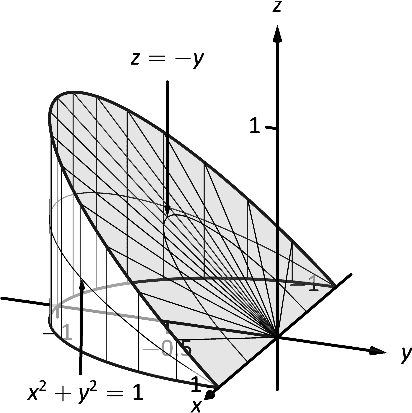
\includegraphics[width=0.4\textwidth]{fig_multiple_25a}}
\qquad
\subfigure[\label{fig_multiple_25b}]{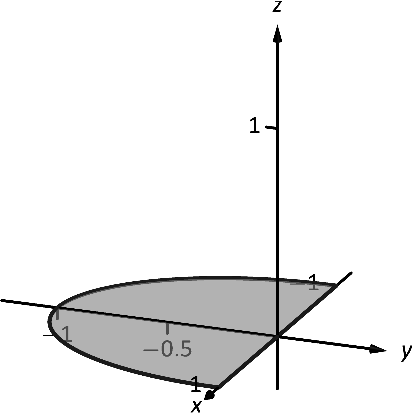
\includegraphics[width=0.4\textwidth]{fig_multiple_25b} }}

%\centerline{\subfigure[\label{fig_multiple_36c}]{\includegraphics[width=0.43\textwidth]{fig_multiple_36c}}
%\qquad
%\subfigure[\label{fig_multiple_36d}]{\includegraphics[width=0.43\textwidth]{fig_multiple_36d} }}
\caption{The region $D$ used in Example \ref{ex_trip3} in (a); the region found by projecting $D$ onto the $xy$-plane (b). %, $xz$- (c) and $yz$- (d) plane.
}
\end{figure}


\end{example}

The following theorem states two things that should make common sense to us. First, using the triple integral to find volume of a region $D$ should always return a positive number; we are computing volume here, not signed volume. Secondly, to compute the volume of a complicated region, we could break it up into subregions and compute the volumes of each subregion separately, summing them later to find the total volume.

\begin{theorem}[Properties of triple integrals]
\label{thm:triple_int_prop}
Let $D$ be a closed, bounded region in space, and let $D_1$ and $D_2$ be non-overlapping regions such that $D=D_1 \cup D_2$.
\index{triple integral!properties}\index{iterated integration!properties}
\begin{enumerate}
	\item $\ds \iiint_D \ dV \geq 0$
	\item	$\ds \iiint_D\ dV = \iiint_{D_1}\ dV + \iiint_{D_2}\ dV.$
\end{enumerate}
\end{theorem}


\begin{example}
\label{ex_trip5}
Set up a triple integral that gives the volume of the space region $D$ bounded by $z=6-2x^2-y^2$ and $z= 2x^2+2$. These surfaces are plotted in Figure \ref{fig_multiple_26a} and (b), respectively; the region $D$ is shown in part (c) of the figure.


\begin{figure}[H]
\centering
%\raisebox{0.5cm}{
\centerline{\subfigure[\label{fig_multiple_26a}]{\includegraphics[width=0.3\textwidth]{fig_multiple_26a}}
\qquad
\subfigure[\label{fig_multiple_26b}]{\includegraphics[width=0.3\textwidth]{fig_multiple_26b} }
\qquad
\subfigure[\label{fig_multiple_26c}]{\includegraphics[width=0.3\textwidth]{fig_multiple_26c} }}

\centerline{\subfigure[\label{fig_multiple_26d}]{\includegraphics[width=0.3\textwidth]{fig_multiple_26d}}
\qquad
\subfigure[\label{fig_multiple_26e}]{\includegraphics[width=0.3\textwidth]{fig_multiple_26e} }}
\caption{The region $D$ in Example \ref{ex_trip5} is bounded by the surfaces shown in (a) and (b); $D$ is shown in (c).%; it is projected onto the $xz$- (d) and $yz$- (e) plane.
}
\end{figure}

\xhrulefill{gray}{2.5pt}Solution \xhrulefill{gray}{2.5pt}

The main point of this example is this: integrating with respect to $z$ first is rather straightforward; integrating with respect to $x$ first is not.

%\noindent The order $dz\ dy\ dx$:\\[0.2cm]
The bounds on $z$ are clearly $2x^2+2\leq z\leq 6-2x^2-y^2$. Projecting $D$ onto the $xy$-plane gives the ellipse shown in Figure \ref{fig_multiple_26c}. The equation of this ellipse is found by setting the two surfaces equal to each other: 
$$2x^2+2 = 6-2x^2-y^2\quad \Leftrightarrow\quad 4x^2+y^2=4\quad \Leftrightarrow\quad x^2+\frac{y^2}4=1.$$


We can describe this ellipse with the bounds 
$$-\sqrt{4-4x^2} \leq y\leq \sqrt{4-4x^2}\quad \text{and}\quad -1\leq x\leq 1.$$ 
Thus the triple integral giving volume is:
$$V= \int\limits_{-1}^1\int\limits_{-\sqrt{4-4x^2}}^{\sqrt{4-4x^2}}\int\limits_{2x^2+2}^{6-2x^2-y^2}\ dz\ dy\ dx .$$

We leave it to the reader to confirm that sticking to the orders of integration $dy\ dz\ dx$ and $dx\ dz\ dy$ requires setting up more complicated integrals. 

%\noindent The order $dy\ dz\ dx$:\\[0.2cm]
%Integrating with respect to $y$ is not too difficult. Since the surface $z=2x^2+2$ is a cylinder whose directrix is the $y$-axis, it does not create a border for $y$. The paraboloid $z=6-2x^2-y^2$ does; solving for $y$, we get the bounds 
%$$-\sqrt{6-2x^2-z}\leq y\leq \sqrt{6-2x^2-z}.$$ 
%Projecting $D$ onto the $xz$-plane gives the region shown in Figure \ref{fig_multiple_37d}; the lower curve is from the cylinder, with equation $z=2x^2+2$. The upper curve is from the paraboloid; with $y=0$, the curve is $z=6-2x^2$. Thus bounds on $z$ are $2x^2+2\leq z\leq 6-2x^2$; the bounds on $x$ are $-1\leq x\leq 1$. Thus we have:
%$$V = \int\limits_{-1}^1\ \int\limits_{2x^2+2}^{6-2x^2}\ \int\limits_{-\sqrt{6-2x^2-z}}^{\sqrt{6-2x^2-z}}\ dy\ dz\ dx. $$



%\noindent The order $dx\ dz\ dy$:\\[0.2cm]

%This order takes more effort as $D$ must be split into two subregions. The two surfaces create two sets of upper/lower bounds in terms of $x$; the cylinder creates bounds $$-\sqrt{z/2-1}\leq x\leq \sqrt{z/2-1}$$ for region $D_1$  and the paraboloid creates bounds $$-\sqrt{3-y^2/2-z/2}\leq x\leq \sqrt{3-y^2/2-z/2}$$ for region $D_2$.


%Projecting $D$ onto the $yz$-plane gives the regions shown in Figure \ref{fig_multiple_37e}. We find the equation of the curve $z=4-y^2/2$ by noting that the equation of the ellipse seen in Figure \ref{fig_multiple_37c} has equation 
%$$x^2+y^2/4=1 \quad \Rightarrow \quad x = \sqrt{1-y^2/4}.$$  
%Substitute this expression for $x$ in either surface equation, $z=6-2x^2-y^2$ or $z=2x^2+2$. In both cases, we find $$z=4-\frac12y^2.$$
%\drawexampleline

%Region $R_1$, corresponding to $D_1$, has bounds 
%$$2\leq z\leq 4-y^2/2\quad \text{and}\quad -2\leq y\leq 2$$ 
%and region $R_2$, corresponding to $D_2$, has bounds 
%$$4-y^2/2\leq z\leq 6-y^2\quad \text{and}\quad -2\leq y\leq 2.$$ 
%Thus the volume of $D$ is given by:
%$$V = \int\limits_{-2}^2\int\limits_2^{4-y^2/2}\int\limits_{-\sqrt{z/2-1}}^{\sqrt{z/2-1}}\ dx\ dz\ dy \ +\ \int\limits_{-2}^2\ \int\limits_{4-y^2/2}^{6-y^2}\int\limits_{-\sqrt{3-y^2/2-z^2/2}}^{\sqrt{3-y^2/2-z^2/2}}\ dx\ dz\ dy.$$

\end{example}

If all one wanted to do in Example \ref{ex_trip5} was find the volume of the region $D$, one would have likely stopped at the first integration setup (with order $dz\ dy\ dx$) and computed the volume from there. However, we included the other two methods 1) to show that it could be done, messy or not, and 2) because sometimes we have to use a less desirable order of integration in order to actually integrate.




\subsection{Functions of three variables}

There are uses for triple integration beyond merely finding volume, just as there are uses for integration beyond area under the curve. These uses start with understanding how to integrate functions of three variables, which is effectively no different than integrating functions of two variables. This leads us to a definition.

\begin{definition}[Iterated integration, (Part II)]
\label{def:triple_integral_2}
Let $D$ be a closed, bounded region in space, over which $g_1(x)$, $g_2(x)$, $f_1(x,y)$, $f_2(x,y)$ and $h(x,y,z)$ are all continuous, and let $a$ and $b$ be real numbers. Then, we may write 
$$\ds \int\limits_a^b\int\limits_{g_1(x)}^{g_2(x)}\int\limits_{f_1(x,y)}^{f_2(x,y)} h(x,y,z)\ dz\ dy\ dx=\int\limits_a^b\int\limits_{g_1(x)}^{g_2(x)}\left(\int\limits_{f_1(x,y)}^{f_2(x,y)} h(x,y,z)\ dz\right) dy\ dx.$$

\index{integration!triple}\index{triple integral}\index{iterated integration}
\end{definition}

But what does a triple integral of a function of three variables mean?  We build up this understanding in a way very similar to how we have understood integration and double integration.

Let $h(x,y,z)$ be a continuous function of three variables, defined over some space region $D$. We can partition $D$ into $n$ rectangular--solid subregions, each with dimensions $\dx_i\times\dy_i\times\ddz_i$. Let $(x_i,y_i,z_i)$ be some point in the $i^{\,\text{th}}$ subregion, and consider the product $h(x_i,y_i,z_i)\dx_i\dy_i\ddz_i$. It is the product of a function value (that is the $h(x_i,y_i,z_i)$ part) and a small volume $\Delta V_i$ (that's the $\dx_i\dy_i\ddz_i$ part). One of the simplest understanding of this type of product is when $h$ describes the density of an object, for then $h\times\text{volume}=\text{mass}$.

We can sum up all $n$ products over $D$. Again letting $\mathcal{D}$ represent the length of the longest diagonal of the $n$ rectangular solids in the partition, we can take the limit of the sums of products as $\mathcal{D}\to 0$. That is, we can find
$$ S = \lim_{\mathcal{D}\to 0} \sum_{i=1}^n h(x_i,y_i,z_i)\Delta V_i=\lim_{\mathcal{D}\to 0} \sum_{i=1}^n h(x_i,y_i,z_i)\dx_i\dy_i\ddz_i.$$

While this limit has lots of interpretations depending on the function $h$, in the case where $h$ describes density, $S$ is the total mass of the object described by the region $D$.

We now use the above limit to define the triple integral, give a theorem that relates triple integrals to iterated iteration, followed by the application of triple integrals to find the centres of mass of solid objects.


\begin{definition}[Triple integral]
\label{def:triple_integral_3}
Let $w=h(x,y,z)$ be a continuous function over a closed, bounded region $D$ in space, and consider any partition of $D$ into $n$ rectangular solids with volume $\Delta V_i$. The triple integral of $h$ over $D$ is
\index{integration!triple}\index{triple integral}\index{iterated integration}
$$\iiint_Dh(x,y,z)\ dV = \lim_{\mathcal{D}\to 0}\sum_{i=1}^n h(x_i,y_i,z_i)\Delta V_i.$$
\end{definition}


The following theorem assures us that the above limit exists for continuous functions $h$ and gives us a method of evaluating the limit.

\begin{theorem}[Triple integration (Part II)]
\label{thm:triple_integration2}
Let $w=h(x,y,z)$ be a continuous function over a closed, bounded region $D$ in space, and let $\Delta D$ be any partition of $D$ into $n$ rectangular solids with volume $V_i$.
\index{integration!triple}\index{triple integral}\index{iterated integration}

\begin{enumerate}
\item		The limit $\ds \lim_{\mathcal{D}\to 0}\sum_{i=1}^n h(x_i,y_i,z_i)\Delta V_i$ exists.

\item		If $D$ is defined as the region bounded by the planes $x=a$ and $x=b$, the cylinders $y=g_1(x)$ and $y=g_2(x)$, and the surfaces $z=f_1(x,y)$ and $z=f_2(x,y)$, where $a<b$, $g_1(x)\leq g_2(x)$ and $f_1(x,y)\leq f_2(x,y)$ on $D$, then
	$$\iiint_D h(x,y,z)\ dV = \int\limits_a^b\int\limits_{g_1(x)}^{g_2(x)}\int\limits_{f_1(x,y)}^{f_2(x,y)} h(x,y,z)\ dz\ dy\ dx.$$

\end{enumerate}
\end{theorem}


Actually, we can view the sum $$\ds \sum_{i=1}^nh(x_i,y_i,z_i)\dx_i\dy_i\ddz_i$$ as a triple sum, $$\sum_{k=1}^p\sum_{j=1}^n\sum_{i=1}^mh(x_i,y_j,z_k)\dx_i\dy_j\ddz_k,$$ which we evaluate as
$$\sum_{k=1}^p\left(\sum_{j=1}^n\left(\sum_{i=1}^mh(x_i,y_j,z_k)\dx_i\right)\dy_j\right)\ddz_k.$$
Here we fix a $k$-value, which establishes the $z$-height of the rectangular solids on one level of all the rectangular solids in the space region $D$. The inner double summation adds up all the volumes of the rectangular solids on this level, while the outer summation adds up the volumes of each level.

This triple summation understanding leads to the $\iiint_D$ notation of the triple integral, as well as the method of evaluation shown in Theorem \ref{thm:triple_integration2}.

 We now apply triple integration to find the centres of mass of solid objects.
 
 
\subsection{Mass and centre of mass}

One may wish to review Section \ref{sec:center_of_mass} for a reminder of the relevant terms and concepts. 

\begin{definition}[Mass, centre of mass of solids]
\label{def:mass_3d}
Let a solid be represented by a closed, bounded region $D$ in space with variable density function $\delta(x,y,z)$. 
\index{moment}\index{center of mass}\index{mass}
\begin{enumerate}
	\item The \textbf{mass} (\textit{massa}) of the object is $\ds M= \iiint_D \ dm=\iiint_D \delta(x,y,z)\ dV$.
	\item	The \textbf{moment about the $yz$-plane} is $\ds M_{yz}=\iiint_D x\delta(x,y,z)\ dV$.
	\item	The \textbf{moment about the $xz$-plane} is $\ds M_{xz}=\iiint_D y\delta(x,y,z)\ dV$.
	\item	The \textbf{moment about the $xy$-plane} is $\ds M_{xy}=\iiint_D z\delta(x,y,z)\ dV$.
	\item The \textbf{centre of mass} (\textit{massamiddelpunt}) of the object is
	$$\big(\overline{x},\overline{y},\overline{z}\big) = \left(\frac{M_{yz}}M,\frac{M_{xz}}M,\frac{M_{xy}}M\right).$$
\end{enumerate}
\end{definition}


\begin{example}
\label{ex_trip8}
Find the centre of mass of the solid represented by the region bounded by the planes $z=0$ and $z=-y$ and the cylinder $x^2+y^2=1$, shown in Figure \ref{fig_multiple_25a}, with density function \\ $\delta(x,y,z) = 10+x^2+5y-5z$. This space region was used in Example \ref{ex_trip3}.


\xhrulefill{gray}{2.5pt}Solution \xhrulefill{gray}{2.5pt}

As we start, consider the density function. It is symmetric about the $yz$- plane, and the farther one moves from this plane, the denser the object is. The symmetry indicates that $\overline x$ should be 0. 


As one moves away from the origin in the $y$- or $z$-directions, the object becomes less dense, though there is more volume in these regions.  

Though none of the integrals needed to compute the centre of mass are particularly hard, they do require a number of steps. We emphasize here the importance of knowing how to set up the proper integrals; in complex situations we can appeal to technology for a good approximation, if not the exact answer. We use the order of integration $dz\ dy\ dx$, using the bounds found in Example \ref{ex_trip3}. As these are the same for all four triple integrals, we explicitly show the bounds only for $M$:
\allowdisplaybreaks
\begin{align*}
M &= \iiint_D \big(10+x^2+5y-5z\big)\ dV \\[0.2cm]
	&= \int\limits_{-1}^1\int\limits_{-\sqrt{1-x^2}}^0\int\limits_0^{-y} \big(10+x^2+5y-5z\big)\ dz\ dy\ dx\\[0.2cm]
	&= \frac{64}5-\frac{15\pi}{16} \approx 3.855,\\[0.2cm]
%\end{align*}
%\begin{align*}
M_{yz}	&= \iiint_D x\big(10+x^2+5y-5z\big)\ dV = 0, \\[0.2cm]%& M_{xy}	&= \iiint_D z\big(10+x^2+5y-5z\big)\ dV & M_{xz}\\
	%&=0\\
M_{xz} &= \iiint_D y\big(10+x^2+5y-5z\big)\ dV\\[0.2cm]
	&= 2-\frac{61\pi}{48}\approx -1.99,\\[0.2cm]
	M_{xy}	&= \iiint_D z\big(10+x^2+5y-5z\big)\ dV \\[0.2cm]
	&= \frac{61\pi}{96}-\frac{10}9\approx 0.885.
\end{align*}
Note how $M_{yz}=0$, as expected. The centre of mass is
$$\big(\overline{x},\overline{y},\overline{z}\big) = \left(0,\frac{-1.99}{3.855},\frac{0.885}{3.855}\right) \approx \big(0,-0.516, 0.230\big).$$
\end{example}


As stated before, there are many uses for triple integration beyond finding volume. When $h(x,y,z)$ describes a rate of change function over some space region $D$, then $$\ds \iiint_D h(x,y,z)\ dV$$ gives the total change over $D$. Our one specific example of this was computing mass; a density function is simply a rate of mass change per volume function. Integrating density gives total mass.

While knowing how to integrate  is important, it is arguably much more important to know how to set up integrals. It takes skill to create a formula that describes a desired quantity; modern technology is very useful in evaluating these formulas quickly and accurately.

In the next section, we learn about two new coordinate systems that allow us to integrate over closed regions in space more easily than when using rectangular coordinates.


\section{Triple integration with cylindrical and spherical coordinates}\label{sec:cylindrical_spherical}

	\checkoddpage
\marginpar{\ifoddpage\hspace*{-1.5cm}\else\hspace*{0.25cm}\fi\includegraphics[width=0.075\textwidth]{youtube}\\
\ifoddpage\hspace*{-1.75cm}\else\hspace*{0.1cm}\fi
\qrcode[height=1.75cm]{https://youtu.be/H7kx98Kw38Y}
%\includegraphics[width=0.1\textwidth]{cilinder_cor}
}

Just as polar coordinates gave us a new way of describing curves in the plane, in this section we will see how cylindrical and spherical coordinates give us new ways of describing surfaces and regions in space.

\pagebreak
\subsection{Cylindrical coordinates}

In short, cylindrical coordinates can be thought of as a combination of the polar and rectangular coordinate systems. One can identify a point $(x_0,y_0,z_0)$, given in rectangular coordinates, with the point $(r_0,\theta_0,z_0)$, given in cylindrical coordinates, where the $z$-value in both systems is the same, and the point $(x_0,y_0)$ in the $xy$-plane is identified with the polar point $P=(r_0,\theta_0)$; see Figure \ref{fig_multiple_27}. So that each point in space that does not lie on the $z$-axis is defined uniquely, we will restrict $r\geq 0$ and $0\leq \theta\leq 2\pi$.



We use the identity $z=z$ along with the identities in Theorem \ref{polarrectangularconversion} to convert between the  rectangular coordinate $(x,y,z)$ and the  cylindrical coordinate $(r,\theta,z)$. More specifically, we have from rectangular to cylindrical:
\begin{equation}
x=r\cos(\theta)\quad y=r\sin(\theta)\quad \text{and}\quad z=z\,.
\label{rectocyl}
\end{equation}
and from cylindrical to rectangular:
\begin{equation}
r=\sqrt{x^2+y^2},\quad \tan(\theta) = \dfrac{y}{x} \quad\text{and}\quad z=z\,,
\label{cyltorect}
\end{equation}

Note that our rectangular to polar conversion formulas (Eq.~\eqref{cyltorect}) used $r^2=x^2+y^2$, allowing for negative $r$-values. Since we now restrict $r\geq 0$, we can use $r=\sqrt{x^2+y^2}$.

\begin{figure}[h]
	\begin{center}
			\includegraphics[width=0.35\textwidth]{fig_multiple_27}
	\caption{Illustrating the principles behind cylindrical coordinates.}
	\label{fig_multiple_27}
	\end{center}
\end{figure}

Setting each of $r$, $\theta$ and $z$ equal to a constant defines a surface in space, as illustrated in the following example.

\begin{example}
\label{ex_cylindrical1}Describe the surfaces $r=1$, $\theta = \pi/3$ and $z=2$, given in cylindrical coordinates.

\xhrulefill{gray}{2.5pt}Solution \xhrulefill{gray}{2.5pt}

The equation $r=1$ describes all points in space that are 1 unit away from the $z$-axis. This surface is a cylinder of radius 1, centred on the $z$-axis. 

The equation $\theta=\pi/3$ describes the plane formed by extending the line $\theta=\pi/3$, as given by polar coordinates in the $xy$-plane, parallel to the $z$-axis.

The equation $z=2$ describes the plane of all points in space that are 2 units above the $xy$-plane. This plane is described by $z=2$ in rectangular coordinates. All three surfaces are graphed in Figure \ref{fig_multiple_28}. Note how their intersection uniquely defines the point $P=(1,\pi/3,2)$.

\begin{figure}[H]
	\begin{center}
			\includegraphics[width=0.4\textwidth]{fig_multiple_28}
	\caption{Graphing the surfaces in cylindrical coordinates from Example \ref{ex_cylindrical1}.}
	\label{fig_multiple_28}
	\end{center}
\end{figure}

\end{example}


Cylindrical coordinates are useful when describing certain domains in space, allowing us to evaluate triple integrals over these domains more easily than if we used rectangular coordinates.

Theorem \ref{thm:triple_integration2} shows how to evaluate $\iiint_Dh(x,y,z)\ dV$ using rectangular coordinates. In that evaluation, we use $dV = dz\,dy\,dx$ (or one of the other five orders of integration). Recall how, in this order of integration, the bounds on $y$ are curve to curve and the bounds on $x$ are point to point: these bounds describe a region $R$ in the $xy$-plane. We could describe $R$ using polar coordinates as done in Section \ref{sec:double_int_polar}. In that section, we saw how we used $dA = r\,dr\,d\theta$ instead of $dA = dy\,dx$. 

Considering the above thoughts, we have $dV = dz\big(r\,dr\,d\theta\big) = r\,dz\,dr\,d\theta$. We set bounds on $z$ as surface to surface as done in the previous section, and then use curve to curve and point to point bounds on $r$ and $\theta$, respectively. Finally, using the identities given above, we change the integrand $h(x,y,z)$ to $h(r,\theta,z)$.

This process should sound plausible; the following theorem states it is truly a way of evaluating a triple integral.

\begin{theorem}[Triple integration in cylindrical coordinates]
\label{thm:triple_int_cylindrical}

Let $w=h(r,\theta,z)$ be a continuous function on a closed, bounded region $D$ in space, bounded in cylindrical coordinates by $\alpha \leq \theta \leq \beta$, $g_1(\theta)\leq r \leq g_2(\theta)$ and $f_1(r,\theta) \leq z \leq f_2(r,\theta)$. Then 
$$\iiint_D h(r,\theta,z)\ dV = \int\limits_\alpha^\beta\int\limits_{g_1(\theta)}^{g_2(\theta)}\int\limits_{f_1(r,\theta)}^{f_2(r,\theta)}h(r,\theta,z) r\,dz\,dr\,d\theta.$$
\end{theorem}


\begin{example}
\label{ex_cylindrical2}Find the mass of the solid represented by the region in space bounded by $z=\sqrt{4-x^2-y^2}+3$, $z=0$ and the cylinder $x^2+y^2=4$ (Figure \ref{fig_multiple_29}), with density function $\delta(x,y,z) = x^2+y^2+z+1$, using a triple integral in cylindrical coordinates. Distances are measured in centimetres and density is measured in g/cm$^3$.

\begin{figure}[H]
	\begin{center}
			\includegraphics[width=0.4\textwidth]{fig_multiple_29}
	\caption{Visualizing the solid used in Example \ref{ex_cylindrical2}.}
	\label{fig_multiple_29}
	\end{center}
\end{figure}

\xhrulefill{gray}{2.5pt}Solution \xhrulefill{gray}{2.5pt}

We begin by describing this region of space with cylindrical coordinates. The plane $z=0$ is left unchanged; with the identity $r=\sqrt{x^2+y^2}$, we convert the hemisphere of radius 2 to the equation $z=\sqrt{4-r^2} + 3$; the cylinder $x^2+y^2=4$ is converted to $r^2=4$, or, more simply, $r=2$.  We also convert the density function: $\delta(r,\theta,z) = r^2+z+1$. To describe this solid with the bounds of a triple integral, we bound $z$ with $0\leq z\leq \sqrt{4-r^2}+3$; we bound $r$ with $0 \leq r \leq 2$; we bound $\theta$ with $0 \leq \theta \leq 2\pi$.

Using Definition \ref{def:mass_3d} and Theorem \ref{thm:triple_int_cylindrical}, we have the mass of the solid is
\begin{align*}
M=\iiint_D\delta(x,y,z)\ dV &= \int\limits_0^{2\pi}\int\limits_0^2\int\limits_0^{\sqrt{4-r^2}+3}\big(r^2+z+1\big)r\,dz\,dr\,d\theta \\[0.2cm]
&= \int\limits_0^{2\pi}\int\limits_0^2\left((r^3+4r)\sqrt{4-r^2}+\frac52r^3+\frac{19}2r\right)\,dr\,d\theta \\[0.2cm]
&= \frac{1318\pi}{15} \approx 276.04\text{ g},
\end{align*}
where we leave the details of the remaining double integral to the reader.
\end{example}



\begin{example}
\label{ex_cylindrical3}
Find the centre of mass of the solid with constant density whose base can be described by the polar curve $r=\cos(3\theta)$ and whose top is defined by the plane $z=1-x+0.1y$, where distances are measured in metres, as seen in Figure \ref{fig_multiple_30}.

\begin{figure}[H]
	\begin{center}
			\includegraphics[width=0.4\textwidth]{fig_multiple_30}
	\caption{Visualizing the solid used in Example \ref{ex_cylindrical3}.}
	\label{fig_multiple_30}
	\end{center}
\end{figure}

\xhrulefill{gray}{2.5pt}Solution \xhrulefill{gray}{2.5pt}


We convert the equation of the plane to use cylindrical coordinates: $z= 1-r\cos(\theta)+0.1r\sin(\theta)$. Thus the region in space is bounded by $0 \leq z \leq 1-r\cos(\theta) + 0.1r\sin(\theta)$, $0 \leq r \leq \cos(3\theta)$, \\ $0 \leq \theta \leq \pi$. Note that the rose curve $r=\cos(3\theta)$ is traced out once on $[0,\pi]$.


Since density is constant, we set $\delta = 1$ and finding the mass is equivalent to finding the volume of the solid. We set up the triple integral to compute this but do not evaluate it; we leave it to the reader to confirm it evaluates to:
$$M = \iiint_D\delta \, dV = \int\limits_0^{\pi}\int\limits_0^{\cos(3\theta)}\ \int\limits_0^{1-r\cos(\theta)+0.1r\sin(\theta)} r\,dz\,dr\,d\theta \approx 0.785.$$

From Definition \ref{def:mass_3d} we set up the triple integrals to compute the moments about the three coordinate planes. The computation of each is left to the reader (using Mathematica is recommended):
\begin{align*}
M_{yz} = \iiint_D x\,\delta\,dV &= \int\limits_0^{\pi}\int\limits_0^{\cos(3\theta)}\ \int\limits_0^{1-r\cos(\theta)+0.1r\sin(\theta)} (r\cos(\theta)) r\,dz\,dr\,d\theta = -0.147, \\[0.2cm]
M_{xz} = \iiint_D y\,\delta\,dV &= \int\limits_0^{\pi}\int\limits_0^{\cos(3\theta)}\ \int\limits_0^{1-r\cos(\theta)+0.1r\sin(\theta)} (r\sin(\theta)) r\,dz\,dr\,d\theta = 0.015,\\[0.2cm]
M_{xy} = \iiint_D z\,\delta\,dV &= \int\limits_0^{\pi}\int\limits_0^{\cos(3\theta)}\ \int\limits_0^{1-r\cos(\theta)+0.1r\sin(\theta)} (z) r\,dz\,dr\,d\theta = 0.467.
\end{align*}
The centre of mass, in rectangular coordinates,  is located at $(-0.147/0.785,0.015/0.785,0.467/0.785)$.
\end{example}

\subsection{Spherical coordinates}

	\checkoddpage
\marginpar{\ifoddpage\hspace*{-1.5cm}\else\hspace*{0.25cm}\fi\includegraphics[width=0.075\textwidth]{youtube}\\
\ifoddpage\hspace*{-1.75cm}\else\hspace*{0.1cm}\fi
\qrcode[height=1.75cm]{https://youtu.be/sT8JIn7Q_Fo}
%\includegraphics[width=0.1\textwidth]{bol_cor}
}

In short, spherical coordinates can be thought of as a double application of the polar coordinate system. In spherical coordinates, a point $P$ is identified with $(\rho,\theta,\varphi)$, where $\rho$ is the distance from the origin to $P$, $\theta$ is the same angle as would be used to describe $P$ in the cylindrical coordinate system, and $\varphi$ is the angle between the positive $z$-axis and the ray from the origin to $P$; see Figure \ref{fig_multiple_31}. So that each point in space that does not lie on the $z$-axis is defined uniquely, we will restrict $\rho \geq 0$, $0 \leq \theta \leq 2\pi$ and $0 \leq \varphi \leq \pi$.
The symbol $\rho$ is the Greek letter rho. Traditionally it is used in the spherical coordinate system, while $r$ is used in the polar and cylindrical coordinate systems.






For comprehensiveness, we list the conversions to/from our three spatial coordinate systems.

\textbf{Rectangular and Cylindrical}
%\parbox{82pt}{$(x,y,z)\rightarrow (r,\theta,z)$:} 
\begin{equation}\begin{array}{c}
r^2 = x^2+y^2,\quad \tan (\theta) = \dfrac{y}{x},\quad z=z\\[0.2cm]
%\parbox{82pt}{$(r,\theta,z)\rightarrow (x,y,z)$:} 
x=r\cos (\theta), \quad y=r\sin(\theta),\quad z=z
\end{array}
\end{equation}

\textbf{Rectangular and Spherical}
\begin{equation}
\begin{array}{c}
\rho = \sqrt{x^2+y^2+z^2},\quad \tan (\theta) = \dfrac{y}{x},\quad \cos (\varphi) = \dfrac{z}{\sqrt{x^2+y^2+z^2}}\\[0.2cm]
x=\rho\sin(\varphi)\cos(\theta),\quad y=\rho\sin(\varphi)\sin(\theta),\quad z=\rho\cos(\varphi)
\end{array}
\end{equation}

\textbf{Cylindrical and Spherical }
\begin{equation}
\begin{array}{c}
\rho=\sqrt{r^2+z^2}, \quad \theta = \theta,\quad \tan (\varphi) = \dfrac{r}{z} \\[0.2cm]
r=\rho \sin (\varphi), \quad \theta = \theta, \quad z=\rho\cos(\varphi)
\end{array}
\end{equation}

\begin{figure}[h]
	\begin{center}
			\includegraphics[width=0.4\textwidth]{fig_multiple_31}
	\caption{Illustrating the principles behind spherical coordinates.}
	\label{fig_multiple_31}
	\end{center}
\end{figure}


\begin{example}
\label{ex_spherical1}Describe the surfaces $\rho=1$, $\theta = \pi/3$ and $\varphi = \pi/6$, given in spherical coordinates.

\xhrulefill{gray}{2.5pt}Solution \xhrulefill{gray}{2.5pt}

The equation $\rho = 1$ describes all points in space that are 1 unit away from the origin: this is the sphere of radius 1, centred at the origin.

The equation $\theta = \pi/3$ describes the same surface in spherical coordinates as it does in cylindrical coordinates: beginning with the line $\theta = \pi/3$ in the $xy$-plane as given by polar coordinates, extend the line parallel to the $z$-axis, forming a plane.

The equation $\varphi=\pi/6$ describes all points $P$ in space where the ray from the origin to $P$ makes an angle of $\pi/6$ with the positive $z$-axis. This describes a cone, with the positive $z$-axis its axis of symmetry, with point at the origin. 

All three surfaces are graphed in Figure \ref{fig_multiple_32}. Note how their intersection uniquely defines the point $P=(1,\pi/3,\pi/6)$.
\begin{figure}[H]
	\begin{center}
			\includegraphics[width=0.4\textwidth]{fig_multiple_32}
	\caption{Graphing the surfaces in spherical coordinates from Example \ref{ex_spherical1}.}
	\label{fig_multiple_32}
	\end{center}
\end{figure}
\vspace*{-0.5cm}
\end{example}


Spherical coordinates are useful when describing certain domains in space, allowing us to evaluate triple integrals over these domains more easily than if we used rectangular coordinates or cylindrical coordinates. The crux of setting up a triple integral in spherical coordinates is appropriately describing the small amount of volume, $dV$, used in the integral.

Considering Figure \ref{fig_multiple_33}, we can make a small spherical wedge by varying $\rho$, $\theta$ and $\varphi$ each a small amount, $\Delta\rho$, $\Delta\theta$ and $\Delta\varphi$, respectively. This wedge is approximately a rectangular solid when the change in each coordinate is small, giving a volume of about
$$\Delta V \approx \Delta\rho\ \times\ \rho\Delta\varphi\ \times\ \rho\sin(\varphi)\Delta\theta.$$

\begin{figure}
	\begin{center}
			\includegraphics[width=0.4\textwidth]{fig_multiple_33}
	\caption{Approximating the volume of a standard region in space using spherical coordinates.}
	\label{fig_multiple_33}
	\end{center}
\end{figure}


Given a region $D$ in space, we can approximate the volume of $D$ with many such wedges. As the size of each of $\Delta\rho$, $\Delta\theta$ and $\Delta\varphi$ goes to zero, the number of wedges increases to infinity and the volume of $D$ is more accurately approximated, giving
$$dV = d\rho\ \times\ \rho\ d\varphi\ \times\ \rho\sin(\varphi)d\theta = \rho^2\sin(\varphi)\ d\rho\ d\theta\ d\varphi.$$

Again, this development of $dV$ should sound reasonable, and the following theorem states it is the appropriate manner by which triple integrals are to be evaluated in spherical coordinates.
Note that it is generally most intuitive to evaluate the triple integral in Theorem \ref{thm:triple_int_spherical} by integrating with respect to $\rho$ first; it often does not matter whether we next integrate with respect to $\theta$ or $\varphi$. As the bounds for these variables are usually constants in practice, it generally is a matter of preference.

\pagebreak
\begin{theorem}[Triple integration in spherical coordinates]
\label{thm:triple_int_spherical}
Let $w=h(\rho,\theta,\varphi)$ be a continuous function on a closed, bounded region $D$ in space, bounded in spherical coordinates by $\alpha_1 \leq \varphi \leq \alpha_2$, $\beta_1 \leq \theta \leq \beta_2$ and $f_1(\theta,\varphi) \leq \rho \leq f_2(\theta,\varphi)$. Then 
$$\iiint_D h(\rho,\theta,\varphi)\ dV = \int\limits_{\alpha_1}^{\alpha_2}\int\limits_{\beta_1}^{\beta_2}\int\limits_{f_1(\theta,\varphi)}^{f_2(\theta,\varphi)} h(\rho,\theta,\varphi) \rho^2\sin(\varphi)\ d\rho\ d\theta\ d\varphi.$$
\end{theorem}


\begin{example}
\label{ex_spherical2}
Let $D$ be the region in space bounded by the sphere, centred at the origin, of radius $r$. Use a triple integral in spherical coordinates to find the volume $V$ of $D$.

\xhrulefill{gray}{2.5pt}Solution \xhrulefill{gray}{2.5pt}

The sphere of radius $r$, centred at the origin, has equation $\rho = r$. To obtain the full sphere, the bounds on $\theta$ and $\varphi$ are $0\leq \theta \leq 2\pi$ and $0 \leq \varphi \leq \pi$. This leads us to:
\allowdisplaybreaks
\begin{align*}
V &= \iiint_D\ dV\\
	&= \int\limits_0^{\pi}\int\limits_0^{2\pi}\int\limits_0^r\big(\rho^2\sin(\varphi)\big)\ d\rho\ d\theta\ d\varphi\\[0.2cm]
	&= \int\limits_0^\pi\int\limits_0^{2\pi}\left(\frac13\rho^3\sin(\varphi)\right)\Bigg|_0^r\ d\theta\ d\varphi\\[0.2cm]
	&= \int\limits_0^\pi\int\limits_0^{2\pi} \left(\frac13r^3\sin(\varphi)\right)\ d\theta\ d\varphi\\[0.2cm]
	&= \int\limits_0^\pi \left(\frac{2\pi}3r^3\sin(\varphi)\right)\ d\varphi\\[0.2cm]
	&= \left.\left(-\frac{2\pi}3r^3\cos(\varphi)\right)\right|_0^{\pi}\\[0.2cm]
	&= \frac{4\pi}3r^3,
\end{align*}
the familiar formula for the volume of a sphere. Note how the integration steps were easy, not using square roots nor integration steps such as substitution.
\end{example}

\begin{example}
\label{ex_spherical3}
Find the centre of mass of the solid with constant density enclosed above by $\rho=4$ and below by $\varphi = \pi/6$, as illustrated in Figure \ref{fig_multiple_34}.


\begin{figure}[H]
	\begin{center}
			\includegraphics[width=0.4\textwidth]{fig_multiple_34}
	\caption{Graphing the solid, and its centre of mass, from Example \ref{ex_spherical3}.}
	\label{fig_multiple_34}
	\end{center}
\end{figure}


\xhrulefill{gray}{2.5pt}Solution \xhrulefill{gray}{2.5pt}

We will set up the four triple integrals needed to find the centre of mass (i.e., to compute $M$, $M_{yz}$, $M_{xz}$ and $M_{xy}$) and leave it to the reader to evaluate each integral. Because of symmetry, we expect the $x$- and $y$- coordinates of the centre of mass to be 0.

While the surfaces describing the solid are given in the statement of the problem, to describe the full solid $D$, we use the following bounds: $0 \leq \rho \leq 4$, $0 \leq \theta \leq 2\pi$ and $0 \leq \varphi \leq \pi/6$. Since density $\delta$ is constant, we assume $\delta =1$.

The mass of the solid is:
\allowdisplaybreaks
\begin{align*}
M &= \iiint_D\ dm = \iiint_D\ dV\\
	&= \int\limits_0^{\pi/6}\int\limits_0^{2\pi}\int\limits_0^4\big(\rho^2\sin(\varphi)\big)\ d\rho\ d\theta\ d\varphi\\[0.2cm]
	&= \frac{64}3\big(2-\sqrt{3}\big)\pi \approx 17.958.
\end{align*}

To compute $M_{yz}$, the integrand is $x$; we use $x = \rho\sin(\varphi)\cos(\theta)$. This gives:
%\drawexampleline
\begin{align*}
M_{yz} &= \iiint_D x\ dm \\
	&= \int\limits_0^{\pi/6}\int\limits_0^{2\pi}\int\limits_0^4 \big((\rho\sin(\varphi)\cos(\theta))\rho^2\sin(\varphi)\big) \ d\rho\ d\theta\ d\varphi\\[0.2cm]
	&= \int\limits_0^{\pi/6}\int\limits_0^{2\pi}\int\limits_0^4 \big(\rho^3\sin^2(\varphi)\cos(\theta)\big) \ d\rho\ d\theta\ d\varphi=0,
\end{align*}
which we expected as we expect $\overline{x} = 0$. Actually, by rewriting the above integral as
\begin{align*}
M_{yz}&= \int\limits_0^{\pi/6}\sin^2(\varphi)\int\limits_0^{2\pi}\cos(\theta)\int\limits_0^4\rho^3 \ d\rho\ d\theta\ d\varphi\\[0.2cm]
&= \int\limits_0^{\pi/6}\sin^2(\varphi) d\varphi\int\limits_0^{2\pi}\cos(\theta)d\theta\int\limits_0^4\rho^3 \ d\rho
\end{align*}
it is immediately clear that it yields $0$ due to the integral of the cosine function over its fundamental period that pops up.

To compute $M_{xz}$, the integrand is $y$. So, we use $y = \rho\sin(\varphi)\sin(\theta)$. This gives:
\begin{align*}
M_{xz} &= \iiint_D y\ dm \\
	&= \int\limits_0^{\pi/6}\int\limits_0^{2\pi}\int\limits_0^4 \big((\rho\sin(\varphi)\sin(\theta))\rho^2\sin(\varphi)\big) \ d\rho\ d\theta\ d\varphi\\[0.2cm]
	&= \int\limits_0^{\pi/6}\int\limits_0^{2\pi}\int\limits_0^4 \big(\rho^3\sin^2(\varphi)\sin(\theta)\big) \ d\rho\ d\theta\ d\varphi =0,
\end{align*}
which we also expected as we expect $\overline{y} = 0$.

To compute $M_{xy}$, the integrand is $z$. So, we use $z = \rho\cos(\varphi)$. This gives:
\begin{align*}
M_{xy} &= \iiint_D z\ dm \\
	&= \int\limits_0^{\pi/6}\int\limits_0^{2\pi}\int\limits_0^4 \big((\rho\cos(\varphi))\rho^2\sin(\varphi)\big) \ d\rho\ d\theta\ d\varphi\\[0.2cm]
	&= \int\limits_0^{\pi/6}\int\limits_0^{2\pi}\int\limits_0^4 \big(\rho^3\cos(\varphi)\sin(\varphi)\big) \ d\rho\ d\theta\ d\varphi\\[0.2cm]
	&=16\pi \approx 50.266.
\end{align*}

Thus the centre of mass is $(0,0,M_{xy}/M) \approx (0,0,2.799)$, as indicated in Figure \ref{fig_multiple_34}. 
\end{example}


This section has provided a brief introduction into two new coordinate systems useful for identifying points in space. Each can be used to define a variety of surfaces in space beyond the canonical surfaces graphed as each system was introduced.

However, the usefulness of these coordinate systems does not lie in the variety of surfaces that they can describe nor the regions in space these surfaces may enclose. Rather,  cylindrical coordinates are mostly used to describe cylinders and spherical coordinates are mostly used to describe spheres. These shapes are of special interest in the sciences, especially in physics, and computations on/inside these shapes is difficult using rectangular coordinates. For instance, in the study of electricity and magnetism, one often studies the effects of an electrical current passing through a wire; that wire is essentially a cylinder, described well by cylindrical coordinates. 

This chapter investigated the natural follow--on to partial derivatives: iterated integration. We learned how to use the bounds of a double integral to describe a region in the plane using both rectangular and polar coordinates, then later expanded to use the bounds of a triple integral to describe a region in space. We used double integrals to find volumes under surfaces, surface area, and the centre of mass of lamina; we used triple integrals as an alternate method of finding volumes of space regions and also to find the centre of mass of a region in space.

Integration does not stop here. We could continue to iterate our integrals, next investigating quadruple integrals whose bounds describe a region in 4--dimensional space. We can also look back to regular integration where we found the area under a curve in the plane. A natural analogue to this is finding the area under a curve, where the curve is in space, not in a plane. These are just two of many avenues to explore under the heading of integration.

	\begin{center}
			\includegraphics[width=0.65\textwidth]{GreatMath_7.jpg}
	\end{center}



\newpage
\section{Exercises}
\renewcommand{\ExerciseListName}{Assignement}

\subsection*{\nameref{sec:iterated_integrals}}
%%%%%%%%%%%%%%%%
%Oefening 1
%%%%%%%%%%%%%%%%
\begin{Exercise} Evaluate the  double integrals below.
    \begin{multicols}{2}
        \Question[difficulty = 1] $\ds \int\limits_1^2\int\limits_{y}^{3y} (x+y)\ dx\ dy$
        \Question[difficulty = 1] $\ds \int\limits_{-1}^2\int\limits_{2x^2-2}^{x^2+x} x\ dy\ dx$
        \Question[difficulty = 2] $\ds \int\limits_{0}^{\pi}\int\limits_{0}^{\cos(\theta)} r \sin(\theta)\ dr\ d\theta$
        \Question[difficulty = 1] $\ds \int\limits_{0}^{\frac{\pi}{2}}\int\limits_{2}^{4\cos(\theta)} r^3\ dr\ d\theta$
        \Question[difficulty = 2] $\ds \int\limits_{0}^1\int\limits_{0}^{1} \dfrac{x^2}{1+y^2}\ dy\ dx$
        \Question[difficulty = 2] $\ds \int\limits_{-1}^{2} \int\limits_0^1 (xy^2 + x^2y)\ dx\ dy$ 
        \Question[difficulty = 2] $\ds \int\limits_0^1\int\limits_{x^2}^{2-x^2} \sqrt{x}y\ dy\ dx$
        \Question[difficulty = 2] $\ds \int\limits_0^{\pi/4}\ \int\limits_{\sin(x)}^{\cos(x)} xy \ dy\ dx$ 
        \EndCurrentQuestion
    \end{multicols}
\end{Exercise}

\setboolean{firstanswerofthechapter}{true}
\begin{Answer}
    \begin{multicols}{2}
    
        \Question $\ds \int\limits_1^2\int\limits_{y}^{3y} (x+y)\ dx\ dy = 14$
        \Question $\ds \int\limits_{-1}^2\int\limits_{2x^2-2}^{x^2+x} x\ dy\ dx = \dfrac{9}{4}$
        \Question $\ds \int\limits_{0}^{\pi}\int\limits_{0}^{\cos(\theta)} r \sin(\theta)\ dr\ d\theta = \dfrac{1}{3}$
        \Question $\ds \int\limits_{0}^{\frac{\pi}{2}}\int\limits_{2}^{4\cos(\theta)} r^3\ dr\ d\theta = 10 \pi$
        \Question $\ds \int\limits_{0}^1\int\limits_{0}^{1} \dfrac{x^2}{1+y^2}\ dy\ dx = \dfrac{\pi}{12}$
        
        \Question $\ds \int\limits_{-1}^{2} \int\limits_0^1 (xy^2 + x^2y)\ dx\ dy = 2$
        
        \Question $\ds \int\limits_0^1\int\limits_{x^2}^{2-x^2} \sqrt{x}y\ dy\ dx = \dfrac{16}{21} $ 
        
        \Question $\ds \int\limits_0^{\pi/4}\ \int\limits_{\sin(x)}^{\cos(x)} xy \ dy\ dx = \dfrac{\pi - 2}{16}$ 
        
    \EndCurrentQuestion
    \end{multicols}
\end{Answer}
\setboolean{firstanswerofthechapter}{false}

%%%%%%%%%%%%%%%%
%Oefening 2
%%%%%%%%%%%%%%%%
\begin{Exercise} Identify the boundaries for the  double integrals below and evaluate.
    \Question[difficulty = 2] $\ds \iint_R\ dA$ \quad  with $R$ the region in the first quadrant between $y^2=x^3$ and $y=x$
    \Question[difficulty = 2] $\ds \iint_R x^2 \ dA$ \quad with $R$ the region in the first quadrant between $xy=16$, $y=x$, $y=0$ and $x=8$
    \Question[difficulty = 2] $\ds \iint_R y\ dA$\quad  with $R$ the region enclosed by $y=x^2$ and $y=x^3$
    \Question[difficulty = 2] $\ds \iint_R \dfrac{1}{\sqrt{2y-y^2}} \ dA$ \quad with $R$ the region enclosed by $x^2=4-2y$ in the first quadrant
    \Question[difficulty = 2] $\ds \iint_R e^{\frac{x}{y}} \ dA$ \quad  with $R$ the region bounded by $y^2=x$, $x=0$ and $y=1$
    \Question[difficulty = 2] $\ds \iint_R e^{-(x+y)} \ dA $ \quad with $R = \left\{ (x,y) \left|\, \dfrac{1}{2}\leq x \leq 1, y \geq 0, x \geq y \right. \right\}$ 
    \Question[difficulty = 3] $\ds \iint_R  \ dA $ \quad with $R = \left\{ (x,y) \left|\, a-y \leq x \leq \sqrt{a^2-y^2}, 0 \leq y \leq a\right. \right\}$ 
    \Question[difficulty = 2] $\ds \iint_R  \dfrac{dA}{x+y} $ \quad with $R$ the triangle with vertices $(0,0)$, $(1,0)$ and $(1,1)$  
\end{Exercise}

\begin{Answer}
        
        \Question $\ds \iint_R\ dA = \ds \int\limits_{0}^1\int\limits_{\sqrt{x^3}}^{x} \ dy\ dx = \ds \int\limits_{0}^1\int\limits_{y}^{\sqrt[3]{y^2}} \ dx\ dy  = \dfrac{1}{10}$
      
        \Question $\ds \iint_R x^2 \ dA =  \ds \int\limits_{0}^4\int\limits_{0}^{x} x^2 \ dy\ dx + \ds \int\limits_{4}^8\int\limits_{0}^{\frac{16}{x}} x^2 \ dy\ dx  = \ds \int\limits_{0}^2\int\limits_{y}^{8}x^2  \ dx\ dy +  \ds \int\limits_{2}^4\int\limits_{y}^{\frac{16}{y}}x^2  \ dx\ dy  = 448$ 
      
         \Question $\ds \iint_R y\ dA = \ds \int\limits_{0}^1\int\limits_{x^3}^{x^2} y\ dy\ dx = \ds \int\limits_{0}^1\int\limits_{\sqrt{y}}^{\sqrt[3]{y}} y\ dx\ dy  = \dfrac{1}{35}$ 
      
         
        \Question $\ds \iint_R \dfrac{1}{\sqrt{2y-y^2}} \ dA  = \ds \int\limits_{0}^2\int\limits_{0}^{\frac{4-x^2}{2}} \dfrac{1}{\sqrt{2y-y^2}}\ dy\ dx = \ds \int\limits_{0}^2\int\limits_{0}^{\sqrt{4-2y}} \dfrac{1}{\sqrt{2y-y^2}}\ dx\ dy  = 4 $ 
      
        \Question $\ds \iint_R e^{\frac{x}{y}} \ dA = \ds\int\limits_{0}^1\int\limits_{\sqrt{x}}^1 e^{\frac{x}{y}}\ dy\ dx = \ds\int\limits_{0}^1\int\limits_{0}^{y^2} e^{\frac{x}{y}}\ dx\ dy = \dfrac{1}{2}$
    
        \Question $\ds \iint_R e^{-(x+y)} \ dA = \ds\int\limits_{1/2}^1\int\limits_0^x e^{-(x+y)}\ dy\ dx  = \ds\int\limits_0^{1/2}\int\limits_{1/2}^1 e^{-(x+y)}\ dx\ dy +  \ds\int\limits_{1/2}^1\int\limits_y^1 e^{-(x+y)}\ dx\ dy$ \\[0.2cm]
        $ = \dfrac{1}{2e^2} - \dfrac{3}{2e} + \dfrac{1}{\sqrt{e}}$ 
        
        \Question $\ds \iint_R  \ dA  = \ds\int\limits_0^a\int\limits_{a-y}^{\sqrt{a^2-y^2}}\ dx \ dy = \ds\int\limits_0^a\int\limits_{a-x}^{\sqrt{a^2-x^2}}\ dy \ dx = \dfrac{a^2}{2}\left( \dfrac{\pi}{2} - 1 \right)$ 
        
        \Question $\ds \iint_R  \dfrac{dA}{x+y} = \ds\int\limits_0^1\int\limits_y^1 \dfrac{1}{x+y} \ dx \ dy = \ds\int\limits_0^1\int\limits_0^x \dfrac{1}{x+y} \ dy \ dx = \ln (2)$ 
    
\end{Answer}

\pagebreak
%%%%%%%%%%%%%%%%
%Oefening 3
%%%%%%%%%%%%%%%% 
\begin{Exercise} Reverse the order of  integration  in the integrals below.
    \begin{multicols}{2}
         \Question[difficulty = 1] $\ds \int\limits_{0}^3\int\limits_{1}^{\sqrt{4-y}} f(x,y)\ dx\ dy$
         \Question[difficulty = 1] $\ds \int\limits_{0}^1\int\limits_{\arccos(y)}^{\frac{\pi}{2}} f(x,y)\ dx\ dy$
         \Question[difficulty = 2] $\ds \int\limits_{-6}^2\int\limits_{\frac{x^2}{4}}^{3-x} f(x,y)\ dy\ dx$
         \Question[difficulty = 3] $\ds \int\limits_{\frac{a}{2}}^{a}\int\limits_{0}^{\sqrt{2ax-x^2}} f(x,y)\ dy\ dx$ \quad with $a>0$ 
         \EndCurrentQuestion
    \end{multicols}
\end{Exercise}

\begin{Answer}
    
         \Question $\ds \int\limits_{0}^3\int\limits_{1}^{\sqrt{4-y}} f(x,y)\ dx\ dy = \ds \int\limits_{1}^2\int\limits_{0}^{4-x^2} f(x,y)\ dy\ dx$
         \Question $\ds \int\limits_{0}^1\int\limits_{\arccos(y)}^{\frac{\pi}{2}} f(x,y)\ dx\ dy = \ds \int\limits_{0}^{\frac{\pi}{2}}\int\limits_{\cos(x)}^{1} f(x,y)\ dy\ dx$
         \Question $\ds \int\limits_{-6}^2\int\limits_{\frac{x^2}{4}}^{3-x} f(x,y)\ dy\ dx = \ds \int\limits_{0}^1\int\limits_{-2\sqrt{y}}^{2\sqrt{y}} f(x,y)\ dx\ dy + \ds \int\limits_{1}^9\int\limits_{-2\sqrt{y}}^{3-y} f(x,y)\ dx\ dy$
         
         \Question $\ds\int\limits_{\frac{a}{2}}^{a}\int\limits_{0}^{\sqrt{2ax-x^2}} f(x,y)\ dy\ dx = \ds\int\limits_0^{\frac{\sqrt{3}a}{2}} \ds \int\limits_{\frac{a}{2}}^{a} f(x,y) \ dx \ dy + \ds \int\limits_{\frac{\sqrt{3}a}{2}}^{a} \ \ds \int\limits_{a-\sqrt{a^2-y^2}}^{a} f(x,y) \ dx \ dy$ 
    
\end{Answer}

%%%%%%%%%%%%%%%%
%Oefening 4
%%%%%%%%%%%%%%%%
\begin{Exercise} Using a double integral, find the area of the regions below.
        \Question[difficulty = 1] the region bounded by $y^2=10x+25$ and $y^2 = -6x+9$
        \Question[difficulty = 3] the region bounded by $x^2+y^2=2x$, $x^2+y^2 = 4x$, $y=x$ and $y=0$
        \Question[difficulty = 2] the region bounded by $r\cos (\theta) = 1$ and $r=2$ (the region that does not contain $r = 0$)
        \Question[difficulty = 3] the region bounded by $r= 1 +\cos (\theta)$ and $r=\cos (\theta)$ 
\end{Exercise}

\begin{Answer}
    
        \Question 
        $A = 2 \ds \int\limits_{0}^{\sqrt{15}}\int\limits_{\frac{25-y^2}{-10}}^{\frac{y^2-9}{-6}} \ dx\ dy = \dfrac{16 \sqrt{15}}{3}$
    
        \Question 
        $A = \ds \int\limits_{1}^{2}\int\limits_{\sqrt{1-(x-1)^2}}^{x} \ dy\ dx + \ds \int\limits_{2}^{4}\int\limits_{0}^{\sqrt{4-(x-2)^2}} \ dy\ dx = 
        \ds \int\limits_{0}^{1}\int\limits_{1+\sqrt{1-y^2}}^{2+\sqrt{4-y^2}} \ dx\ dy + \ds \int\limits_{1}^{2}\int\limits_{y}^{2+\sqrt{4-y^2}} \ dx\ dy $ \\[0.2cm]
        $= \ds \int \limits_0^{\frac{\pi}{4}} \int\limits_{2 \cos(\theta)}^{4\cos(\theta)} \ r \ dr \ d\theta= \dfrac{3 \pi }{4} + \dfrac{3}{2} $
        
        \Question 
         $A = 2 \ds \int\limits_{0}^{\frac{\pi}{3}}\int\limits_{\frac{1}{\cos (\theta)}}^{2} r\ dr\ d\theta = \dfrac{4 \pi }{3} - \sqrt{3}$
        
        \Question 
         $A = 2 \ds \int\limits_{0}^{\pi}\int\limits_{0}^{1 + \cos(\theta)} r\ dr\ d\theta - 2 \ds \int\limits_{0}^{\frac{\pi}{2}}\int\limits_{0}^{\cos(\theta)} r\ dr\ d\theta = \dfrac{5 \pi }{4}$
         
    
\end{Answer}

\subsection*{\nameref{sec:double_int_volume}}
%%%%%%%%%%%%%%%%
%Oefening 5
%%%%%%%%%%%%%%%%   
%Volume in cart coord 
\begin{Exercise} Find the volume of the solids below using Cartesian coordinates.
        \Question[difficulty = 2] the solid enclosed by the three coordinate planes and the surfaces \\ $x^2+4y^2=4$ and $y^2+2z=4$
        \Question[difficulty = 2] the solid enclosed by the three coordinate planes and the surfaces \\ $z=1-x^2-y^2$ and $x+y \leq 1$
        \Question[difficulty = 3]the solid enclosed by the coordinate   planes  and the surfaces $y=x^2$, $x=y^2$, $z=0$ en $z=12 + y - x^2$
        \Question[difficulty = 3] the frustum with  side faces $x=0$, $x=2$, $y=0$, $y=1$,  base $z=0$ and top face $-x+y+2z=4$ 
        \Question[difficulty = 2] the solid enclosed by $x^2+y^2=1$ and $x^2+z^2=1$ 
\end{Exercise}

\begin{Answer}
    
        \Question
        $V = \ds \int\limits_0^2 \ds \int\limits_0^{\frac{\sqrt{4-x^2}}{2}} \dfrac{4-y^2}{2} \ dy \ dx   = \ds \int\limits_0^1 \ds \int\limits_0^{2\sqrt{1-y^2}} \dfrac{4-y^2}{2} \ dx\ dy = \dfrac{15 \pi}{16}$
        \Question $V =\ds \int\limits_0^1 \ds \int\limits_0^{1-x} (1-x^2-y^2) \ dy \ dx= \ds \int\limits_0^1 \ds \int\limits_0^{1-y} (1-x^2-y^2) \ dx \ dy = \dfrac{1}{3}$
        \Question $V = \ds \int\limits_0^1 \ds \int\limits_{x^2}^{\sqrt{x}} (12+y-x^2) \ dy \ dx=  \ds \int\limits_0^1\ds \int\limits_{y^2}^{\sqrt{y}} (12+y-x^2) \ dx \ dy = \dfrac{569}{140}$

        \Question $V = \ds \int\limits_0^2 \ds \int\limits_{0}^{1} \dfrac{4+x-y}{2} \ dy\  dx=  \ds \int\limits_0^1\ds \int\limits_{0}^{2} \dfrac{4+x-y}{2}  \ dx\  dy = \dfrac{9}{2} $
        
        \Question $V = 8 \ds \int\limits_0^1 \ds \int\limits_{0}^{\sqrt{1-x^2}} \sqrt{1-x^2} \ dy\  dx = 8 \ds \int\limits_0^1\ds \int\limits_{0}^{\sqrt{1-y^2}} \sqrt{1-x^2}  \ dx\  dy = \dfrac{16}{3} $
         
    
\end{Answer}

%%%%%%%%%%%%%%%%
%Oefening 6
%%%%%%%%%%%%%%%%
\begin{Exercise} Find the volume of the solids below using polar coordinates
     \Question[difficulty = 2] the solid within $x^2+y^2=1$, cut off by $x^2+y^2+z^2=4$ 
     \Question[difficulty = 3] the solid inside $x^2+y^2=2az\, (a>0)$, cut off by $x^2+y^2+z^2=3a^2$ 
     \Question[difficulty = 2] the solid enclosed by $x^2+y^2+z^2=a^2$ and $x^2+y^2=ax$ 
     \Question[difficulty = 3] the solid enclosed by $x^2+y^2=2y$ and $z^2=y$ 
\end{Exercise}

\begin{Answer}
    
        \Question $V = 8 \ds \int\limits_0^{\frac{\pi}{2}} \ds \int\limits_0^{1} \sqrt{4 - r^2}\, r \ dr\ d\theta  = \dfrac{4 \pi}{3}\left(8-3\sqrt{3}\right)$

        \Question $V = \ds \int\limits_0^{a\sqrt{2}} \ds \int\limits_0^{2\pi} \left(\sqrt{3a^2-r^2} - \dfrac{r^2}{2a}  \right)\, r\ d\theta \ dr = \dfrac{a^3\pi}{3}\left( 6\sqrt{3} - 5 \right)$

        \Question $V = 4 \ds \int\limits_0^{\frac{\pi}{2}} \ds \int\limits_0^{a\cos(\theta)} \sqrt{a^2 - r^2}\, r \ dr \ d\theta  = \dfrac{4}{3}a^3 \left(- \dfrac{2}{3} + \dfrac{\pi}{2} \right)$
        
        \Question $V = 4 \ds \int\limits_0^{\frac{\pi}{2}} \ds \int\limits_0^{2\sin(\theta)} \sqrt{r \sin(\theta)}\, r  \ dr \ d\theta = \dfrac{64 \sqrt{2}}{15}$
    
    
\end{Answer}

\pagebreak
\subsection*{\nameref{sec:afl_Leibniz}}
%%%%%%%%%%%%%%%%
%Oefening 7 
%%%%%%%%%%%%%%%%
\begin{Exercise} Find the derivatives below.
\begin{multicols}{2}
    \Question[difficulty = 1] $\dfrac{d}{dt} \left( \ds \int\limits_{0}^1 \sin (x-t)\ dx \right)$ %boek Ottoy hfdstk 15 vb
    \Question[difficulty = 2] $\dfrac{d}{dt} \left( \ds \int\limits_{1}^{t^2} \dfrac{e^{tx}}{x} \ dx \right)$ 
    \Question[difficulty = 3] $\dfrac{d}{dx} \left( \ds \int\limits_{\frac{1}{x}}^{\frac{2}{x}} \dfrac{\sin (tx)}{t} \ dt \right)$ 
    \EndCurrentQuestion
\end{multicols}
\end{Exercise}

\begin{Answer}
    
        \Question $\dfrac{d}{dt} \left( \ds \int\limits_{0}^1 \sin (x-t)\ dx \right) = -\sin(1-t)-\sin(t)$ 
        \Question $\dfrac{d}{dt} \left( \ds \int\limits_{1}^{t^2} \dfrac{e^{tx}}{x} \ dx \right) = 3\dfrac{e^{t^3}}{t} - \dfrac{e^{t}}{t} $ 
        \Question $\dfrac{d}{dx} \left( \ds \int\limits_{\frac{1}{x}}^{\frac{2}{x}} \dfrac{\sin (tx)}{t} \ dt \right)=0$ 
       
    
\end{Answer}

%%%%%%%%%%%%%%%%
%Oefening 8
%%%%%%%%%%%%%%%%
\begin{Exercise}[difficulty = 3] Evaluate the following integrals.
\begin{multicols}{2}
    \Question $F(\alpha) = \ds \int\limits_{0}^{+\infty} e^{-x} \dfrac{\sin(\alpha x)}{x} \ dx $
    \Question $F(a)=\ds \int\limits_0^{+\infty} \dfrac{e^{-ax} \sin (x)}{x} \; dx $ %Oef 11(a) uit H12
    \Question $F(a)=\ds \int\limits_0^{1} \dfrac{x^a - 1}{\ln (x)} \; dx $ %Oef 11(b) uit H12
        \EndCurrentQuestion
\end{multicols}
\end{Exercise}

\begin{Answer}
    First we derive both limits to $\alpha$:
    \[F'(\alpha) = \ds \int\limits_{0}^{+\infty} \dfrac{\partial}{\partial \alpha} \left( e^{-x} \dfrac{\sin(\alpha x)}{x} \right) \ dx = \dfrac{1}{\alpha^2 + 1}. \]
    Integrating this result to $\alpha$ results in $\arctan(\alpha) + C$. As $F(0)=0$, is $C=0$. Therefor we conclude $F(\alpha) = \arctan(\alpha)$.
    \\ $I=\arctan\left(\dfrac{1}{a}\right) $
    \\ $I= \ln|a+1|$
\end{Answer}

\subsection*{\nameref{sec:center_of_mass}}
%%%%%%%%%%%%%%%%
%Oefening 9
%%%%%%%%%%%%%%%%
\begin{Exercise} Find the center of mass of the considered region with the given mass density.
        \Question[difficulty = 1]  the flat region enclosed by$y= \sin (x)$ en $y=0 \ (0\leq x \leq \pi)$ with mass density \\ $\delta(x,y) = ky$. 
        \Question[difficulty = 2]  the flat region enclosed by $y^2 = 4x + 4$ and $y^2 = -2x+4$ with mass density $\delta = 1$ 
        \Question[difficulty = 2]  a triangular plate defined by the region enclosed by the $x$- and $y$-axis and the line $2x+3y=12$ with mass density $\delta = 1$
\end{Exercise}

\begin{Answer}
    
        \Question  
        \begin{itemize}
            \item $M = \ds \int\limits_0^{\pi}\int\limits_{0}^{\sin(x)}ky \ dy\  dx = \dfrac{k \pi}{4}$ 
            \item $M_{y} = k \ds \int\limits_0^{\pi}\int\limits_{0}^{\sin(x)} xy \ dy\  dx = \dfrac{k \pi^2}{8} \quad \Rightarrow \overline{x} = \dfrac{\pi}{2}$
            \item $M_{x} = k \ds \int\limits_0^{\pi}\int\limits_{0}^{\sin(x)} y^2 \ dy\  dx = \dfrac{4 k }{9}  \quad \Rightarrow \overline{y} = \dfrac{16}{9\pi} $
        \end{itemize}
         Center of mass: $\left(\dfrac{\pi}{2}, \dfrac{16}{9\pi}\right)$
        
        \Question  
        \begin{itemize}
            \item $M = \ds \int\limits_{-2}^{2} \ds \int\limits_{\frac{y^2-4}{4}}^{\frac{y^2-4}{-2}} 1 \ dx\  dy = 8$ 
            \item $M_{y} = \ds \int\limits_{-2}^{2}\ds \int\limits_{\frac{y^2-4}{4}}^{\frac{y^2-4}{-2}} x \ dx\  dy = \dfrac{16}{5} \quad \Rightarrow \overline{x} = \dfrac{2}{5}$ 
            \item $M_{x} = \ds \int\limits_{-2}^{2}\ds \int\limits_{\frac{y^2-4}{4}}^{\frac{y^2-4}{-2}} y \ dx\  dy = 0 \quad \Rightarrow \overline{y} = 0 $ 
        \end{itemize}
        Center of mass: $\left(\dfrac{2}{5}, 0\right)$
        
        \Question
        \begin{itemize}
            \item $M = \ds \int\limits_0^{4} \ds \int\limits_{0}^{\frac{12-3y}{2}} 1 \ dx\  dy = 12$ 
            \item $M_{y} = \ds \int\limits_0^{4} \ds \int\limits_{0}^{\frac{12-3y}{2}} x \ dx\  dy = 24 \quad \Rightarrow \overline{x} = 2$ 
            \item $M_{x} = \ds \int\limits_0^{4} \ds \int\limits_{0}^{\frac{12-3y}{2}} y \ dx\  dy = 16 \quad \Rightarrow \overline{y} = \dfrac{4}{3}$
        \end{itemize}
        Center of mass: $\left(2,\dfrac{4}{3}\right)$
        
    
\end{Answer}  


\subsection*{\nameref{sec:surface_area}}
%%%%%%%%%%%%%%%%
%Oefening 10
%%%%%%%%%%%%%%%%
\begin{Exercise} Find the surface area of the solids below.
    \Question[difficulty = 3] the part of $x^2+y^2 = 3z^2$, that lies above the $xy$-plane and inside $x^2+y^2=4y$
    \Question[difficulty = 2] the part of $x^2+z^2=16$, that lies inside $x^2+y^2=16$
    \Question[difficulty = 3] the part of $z^2=4x$, that lies inside $y^2=4x$ and $x \leq 1$
    \Question[difficulty = 2] the part of $z=1-x^2-y^2$, that lies inside $x^2+y^2=1$
    \Question[difficulty = 2] the part of $x^2+y^2+z^2= a^2$  cut off by $x^2+4y^2=a^2$.
\end{Exercise}

\begin{Answer}
    
    \Question $SA=2 \ds \int\limits_0^{\frac{\pi}{2}} \int\limits_0^{4 \sin(\theta) } \dfrac{2}{\sqrt{3}} \, r \  dr \ d\theta = \dfrac{8 \pi}{\sqrt{3}}$
    \Question $SA=8 \ds \int\limits_0^{4} \int\limits_0^{\sqrt{16-x^2}} \sqrt{\dfrac{16}{16-x^2}}  \  dy \ dx = 128 $
    
    \Question $SA=4 \ds \int\limits_0^{1} \int\limits_0^{2\sqrt{x}} \sqrt{\dfrac{x+1}{x}}  \  dy \ dx = \dfrac{16}{3} \left(2 \sqrt{2}-1 \right) $
    
    \Question $SA= \ds \int\limits_0^{2\pi} \int\limits_0^{1} \sqrt{1+4r^2} \ r \ dr \ d\theta = \dfrac{\pi}{6} \left(5\sqrt{5}-1 \right) $
    
    \Question $SA= 8 \ds \int\limits_0^{a} \int\limits_0^{\frac{\sqrt{a^2 - x^2}}{2}} \sqrt{ \dfrac{a^2}{a^2-x^2-y^2}} \ dy \ dx = \dfrac{4a^2\pi}{3}$
    
    
\end{Answer}



\subsection*{\nameref{sec:triple_int}}
%%%%%%%%%%%%%%%%%%%%%%%%
%DRIEVOUDIGE INTEGRALEN
%%%%%%%%%%%%%%%%%%%%%%%%


%%%%%%%%%%%%%%%%
%Oefening 12
%%%%%%%%%%%%%%%%
\begin{Exercise} Evaluate the  triple integrals below.
    \Question[difficulty = 2] $\ds \iiint_D xyz\ dV$ \quad with $D$ the solid enclosed by the coordinate planes and the plane \\ $x+y+z=1$ \\[0.1cm] 
    \Question[difficulty = 2] $\ds \iiint_D (x+z) \ dV $ \quad with $D = \left\{ (x,y,z) \left|\, 0\leq x, 0 \leq y, 0 \leq z, x^2 + y^2 + z^2 \leq 1 \right. \right\}$ \\[0.1cm]  
    \Question[difficulty = 3] $\ds \iiint_D xy \ dV $ \quad with $D = \left\{ (x,y,z) \left|\, 0\leq x, 0 \leq y, 0 \leq z \leq 1, x^2 + y^2 \leq 1 \right. \right\}$ \\[0.1cm]  
    \Question[difficulty = 3] $\ds \iiint_D \left( x^2 + y^2 + z^2 \right)^{3/2} \ dV $ \quad with $D = \left\{ (x,y,z) \left|\,  x^2 + y^2 + z^2 \leq 1 \right. \right\}$ \\[0.1cm]  
\end{Exercise}

\begin{Answer}
    
        \Question $\ds \int\limits_0^{1} \int\limits_{0}^{1-z}\ \int\limits_{0}^{1-y-z} xyz \ dx\  dy \ dz = \dfrac{1}{720}$
        
        \Question $\ds \int\limits_0^{1} \int\limits_{0}^{\sqrt{1-z^2}}\ \int\limits_{0}^{\sqrt{1-y^2-z^2}} (x+z) \ dx\  dy \ dz = \dfrac{\pi}{8}$
       
        \Question $\ds \int\limits_0^{1} \int\limits_{0}^{1}\ \int\limits_{0}^{\sqrt{1-y^2}} xy \ dx\  dy \ dz = \dfrac{1}{8}$
        
        \Question $8 \ds \int\limits_0^{1} \int\limits_{0}^{\sqrt{1-z^2}}\ \int\limits_{0}^{\sqrt{1-y^2-z^2}} \left( x^2 + y^2 + z^2 \right)^{3/2} \ dx\  dy \ dz = \dfrac{2\pi}{3}$
    
\end{Answer}


\subsection*{\nameref{sec:cylindrical_spherical}}
%%%%%%%%%%%%%%%%
%Oefening 13
%%%%%%%%%%%%%%%%
\begin{Exercise} Find the volume of the solids below using the most appropriate coordinate system.
    \Question[difficulty = 3] the solid enclosed by $z=10-x^2-y^2$ and $z=2(x^2+y^2-1)$ 
    \Question[difficulty = 2] the solid inside the ellipsoid $\dfrac{x^2}{a^2} + \dfrac{y^2}{b^2} + \dfrac{z^2}{c^2} = 1$ 
    \Question[difficulty = 2] the solid above the $xy$-plane, under $x^2 + y^2 + 2z = 16$ and within $x^2 + y^2 = 4$ 
    \Question[difficulty = 3] the solid inside $3(x^2+y^2) = z^2$, cut off by $x^2+y^2+z^2=a^2$
    \Question[difficulty = 2] the solid enclosed by $x^2+y^2 + z^2 = 4$ and $x^2+y^2=3z$ 
\end{Exercise}

\begin{Answer}
    
        \Question $V = \ds\int\limits_0^2\int\limits_0^{2\pi}\int\limits_{2\left(r^2-1\right)}^{10-r^2} \, r\ dz\ d\theta \ dr =  24\pi$
        
        \Question $V = \ds\int\limits_{-a}^{+a} \ \ds\int\limits_{-b\sqrt{1 - \frac{x^2}{a^2}}}^{b\sqrt{1 - \frac{x^2}{a^2}}} \ \ds\int\limits_{-c\sqrt{1 - \frac{x^2}{a^2} - \frac{y^2}{b^2}}}^{c\sqrt{1 - \frac{x^2}{a^2} - \frac{y^2}{b^2}}} \ dz \ dy \ dx = \dfrac{4}{3} \pi a b c $
        
        \Question $V = \ds \int\limits_0^2\int\limits_0^{2\pi}\int\limits_0^{\frac{16-r^2}{2}} \, r \ dz \ d\theta \ dr =  28\pi$
        
        \Question $V = 2\ds \int\limits_0^{2\pi} \int\limits_0^a  \int\limits_0^{\frac{\pi}{6}} \rho^2 \sin(\varphi) \ d\varphi \ d\rho \ d\theta = \dfrac{4\pi a^3}{3}\left(1-\dfrac{\sqrt{3}}{2}\right)$
        
        \Question $V = \ds\int\limits_0^{2\pi}\int\limits_0^{\sqrt{3}}\int\limits_{\frac{r^2}{3}}^{\sqrt{4-r^2}} \, r\ dz\ dr \ d\theta = \dfrac{19\pi}{6}$
        
    
\end{Answer}

\subsection*{Review exercises}
%%%%%%%%%%%%%%%%
%Oefening 11
%%%%%%%%%%%%%%%%
\begin{Exercise}[difficulty = 3] Find the volume of a building that has its roof at height $z=\arctan \left( yx^{-1} \right)$, the $xy$-plane as a base and  shape defined by $x^2+y^2=1$, with $x \geq 0$ and $y \geq 0$. What is the area of the roof? 
\end{Exercise}

\begin{Answer}
    $V = \ds \int\limits_0^1 \int\limits_0^{\frac{\pi}{2}} \theta \, r\ d\theta \ dr = \dfrac{\pi^2}{16}, \quad SA = \ds \int\limits_0^1 \int\limits_0^{\frac{\pi}{2}} \sqrt{1 + \dfrac{1}{r^2}}\ r \ d\theta \ dr =  \dfrac{\pi}{4}\left( \sqrt{2} + \ln \left(\sqrt{2}+1\right) \right) $
\end{Answer}

%%%%%%%%%%%%%%%%
%Oefening 14
%%%%%%%%%%%%%%%%
\begin{Exercise}[difficulty = 3] At the campsite of a festival, there are many tents. These have a square base (in the $xy$-plane) and are enclosed by two  parabolic cylinders $ax^2+z=a$ and $ay^2+z=a$. What is the volume of such a tent?
\end{Exercise}

\begin{Answer}
    $V = \ds\int\limits_0^a \int\limits_{-\sqrt{\frac{a-z}{a}}}^{\sqrt{\frac{a-z}{a}}} \int\limits_{-\sqrt{\frac{a-z}{a}}}^{\sqrt{\frac{a-z}{a}}} \ dx dy dz =2a$
\end{Answer}

%%%%%%%%%%%%%%%%
%Oefening 15
%%%%%%%%%%%%%%%%
\begin{Exercise} Find the center of mass of the solids below with the given mass density.
    \Question[difficulty = 3] the upper part of the cone $x^2 + y^2 = z^2$ above $z=h \ (h>0)$ and with mass density $\delta(x,y,z) = 1 - \dfrac{z}{h}$ 
    \Question[difficulty = 2]  the solid enclosed by $z=x^2+y^2$ and $z=4$ and with mass density \\ $\delta(x,y,z) = k \sqrt{x^2 + y^2}$. 
    \Question[difficulty = 3] the surface $x^2 + y^2 - z^2 = 1$ between $z=0$ and $z=2$ and with mass density $\delta = 1$ 
\end{Exercise}

\begin{Answer}
    
        \Question Cylindrical coordinates:
        \begin{itemize}
            \item $M = \ds\int\limits_0^{2\pi}\int\limits_0^h\int\limits_r^h \left(1-\dfrac{z}{h}\right)\, r\ dz\ dr\ d\theta   = \dfrac{h^3\pi}{12}$
            \item $M_{yz} = \ds\int\limits_0^{2\pi}\int\limits_0^h\int\limits_r^h r\cos(\theta)\left(1-\dfrac{z}{h}\right)\, r\ dz \ dr \ d\theta  = 0 \quad \Rightarrow \overline{x} = 0$ 
            \item $M_{xz} = \ds\int\limits_0^{2\pi}\int\limits_0^h\int\limits_r^h r\sin(\theta)\left(1-\dfrac{z}{h}\right)r\ dz \ dr \ d\theta  = 0 \quad \Rightarrow \overline{y} = 0$ 
            \item $M_{xy} = \ds\int\limits_0^{2\pi}\int\limits_0^h\int\limits_r^h z\left(1-\dfrac{z}{h}\right)r\ dz \ dr \ d\theta  = \dfrac{h^4\pi}{20} \quad  \Rightarrow \overline{z} = \dfrac{3h}{5}$ 
            \end{itemize}
            Center of mass: $\left(0,0,\dfrac{3h}{5}\right)$
            
         Spherical coordinates:
        \begin{itemize}
            \item $M = \ds\int\limits_0^{2\pi}\int\limits_0^{\frac{\pi}{4}}\int\limits_0^{\frac{h}{\cos(\varphi)}} \left(1-\dfrac{\rho \cos(\varphi)}{h}\right)\rho^2 \sin(\varphi)\ d\rho \ d\varphi \ d\theta   = \dfrac{h^3\pi}{12}$
            \item $M_{yz} = \ds\int\limits_0^{2\pi}\int\limits_0^{\frac{\pi}{4}}\int\limits_0^{\frac{h}{\cos(\varphi)}} \rho \sin(\varphi)\cos(\theta) \left(1-\dfrac{\rho \cos(\varphi)}{h}\right)\rho^2 \sin(\varphi)\ d\rho \ d\varphi \ d\theta  = 0$ 
            \item $M_{xz} = \ds\int\limits_0^{2\pi}\int\limits_0^{\frac{\pi}{4}}\int\limits_0^{\frac{h}{\cos(\varphi)}} \rho \sin(\varphi)\sin(\theta) \left(1-\dfrac{\rho \cos(\varphi)}{h}\right)\rho^2 \sin(\varphi)\ d\rho \ d\varphi \ d\theta  = 0 $ 
            \item $M_{xy} = \ds\int\limits_0^{2\pi}\int\limits_0^{\frac{\pi}{4}}\int\limits_0^{\frac{h}{\cos(\varphi)}} \rho \cos(\varphi)\left(1-\dfrac{\rho \cos(\varphi)}{h}\right)\rho^2 \sin(\varphi)\ d\rho \ d\varphi \ d\theta   = \dfrac{h^4\pi}{20}$ 
            \end{itemize}
    
        \Question  \begin{itemize}
            \item $M = \ds\int\limits_0^{2\pi}\int\limits_0^2\int\limits_{r^2}^4 kr \, r\ dz\ dr\ d\theta   = \dfrac{128k\pi}{15}$
            \item $M_{yz} = \ds\int\limits_0^{2\pi}\int\limits_0^2\int\limits_{r^2}^4 r \cos(\theta) kr \, r\ dz\ dr\ d\theta   = 0 \quad \Rightarrow \overline{x} = 0$ 
            \item $M_{xz} = \ds\int\limits_0^{2\pi}\int\limits_0^2\int\limits_{r^2}^4 r \sin(\theta) kr \, r\ dz\ dr\ d\theta   = 0 \quad \Rightarrow \overline{y} = 0$ 
            \item $M_{xy} = \ds\int\limits_0^{2\pi}\int\limits_0^2\int\limits_{r^2}^4 z kr \, r\ dz\ dr\ d\theta   = \dfrac{512k\pi}{21} \quad \Rightarrow \overline{z} = \dfrac{20}{7}$ 
            \end{itemize}
            Center of mass: $\left(0,0,\dfrac{20}{7}\right)$
        
        \Question 
        \begin{itemize}
            \item $M = \ds\int\limits_0^{2\pi}\int\limits_0^2\int\limits_{0}^{\sqrt{1+z^2}}\, r\ dr\ dz\ d\theta   = \dfrac{14\pi}{3}$
            \item $M_{yz} = \ds\int\limits_0^{2\pi}\int\limits_0^2\int\limits_{0}^{\sqrt{1+z^2}} r \cos(\theta)\, r\ dr\ dz\ d\theta    = 0 \quad \Rightarrow \overline{x} = 0$ 
            \item $M_{xz} = \ds\int\limits_0^{2\pi}\int\limits_0^2\int\limits_{0}^{\sqrt{1+z^2}} r \sin(\theta)\, r\ dr\ dz\ d\theta  = 0 \quad \Rightarrow \overline{y} = 0$ 
            \item $M_{xy} = \ds\int\limits_0^{2\pi}\int\limits_0^2\int\limits_{0}^{\sqrt{1+z^2}} z \, r\ dr\ dz\ d\theta   = 6 \pi \quad \Rightarrow \overline{z} = \dfrac{9}{7}$ 
            \end{itemize}
            Center of mass: $\left(0,0,\dfrac{9}{7}\right)$
        
    
\end{Answer}